% !TEX root = ../../tcc.tex

\chapter{Proposta do Cognita}
\label{cap:proposta}

% Evita o espaçamento vertical esticado quando tabelas fixas [H] vão para a página seguinte.
\raggedbottom

O planejamento do Cognita, módulo de estimativa do domínio de conceitos a ser incorporado ao Ecossistema CEDIS, compreende o alinhamento da visão do produto por meio da \textit{Lean Inception}, a especificação dos requisitos funcionais e não funcionais, a definição da arquitetura de integração, a modelagem das entidades e atributos de entrada, a prototipação das interfaces e o cronograma de desenvolvimento em ondas.


\section{Visão do Produto}
\label{sec:visao-produto}

Os artefatos de alinhamento estratégico produzidos durante a aplicação adaptada da \textit{Lean Inception} \cite{caroli_lean_2018} sustentam o levantamento e a priorização dos requisitos do módulo Cognita, orientando a definição do Produto Mínimo Viável (MVP) em consonância com as restrições arquiteturais e de privacidade do ecossistema.

A Figura~\ref{fig:logo-cognita} apresenta a logomarca do módulo, na qual a peça de quebra-cabeça representa que o Cognita é um módulo integrado ao Ecossistema CEDIS, e não um software independente.

\begin{figure}[htb]
\caption{Logomarca do módulo Cognita}
\label{fig:logo-cognita}
\centering

\includegraphics[width=0.7\textwidth]{figuras/CognitaLogo.png}
\legend{Fonte: Elaborado pelos autores.}
\end{figure}

\subsection{Visão e Escopo}
\label{subsec:visao-escopo}

A primeira atividade da \textit{Lean Inception} consistiu na construção colaborativa da Declaração de Visão do Produto. O objetivo desse artefato é estabelecer um entendimento unificado sobre o propósito do módulo Cognita dentro do Ecossistema CEDIS, explicitando os segmentos de usuários atendidos, o problema central de diagnóstico pedagógico, a categoria técnica da solução, os benefícios esperados e o seu diferencial perante soluções de mercado \cite{caroli_lean_2018}.

A partir do mapeamento das limitações analíticas atuais do ecossistema, que se concentra em métricas descritivas de engajamento e não acompanha longitudinalmente o domínio dos estudantes, identificou-se que o problema central manifesta-se em duas frentes complementares: a dificuldade do estudante em reconhecer com precisão suas próprias lacunas conceituais e a dificuldade do docente em diagnosticar quais conceitos específicos apresentam baixa absorção na turma. A Figura~\ref{fig:visao-produto} apresenta o quadro resultante da dinâmica de Visão do Produto realizada na \textit{Lean Inception}.

\begin{figure}[htb]
\caption{Artefato da atividade de Visão do Produto na \textit{Lean Inception}}
\label{fig:visao-produto}
\centering
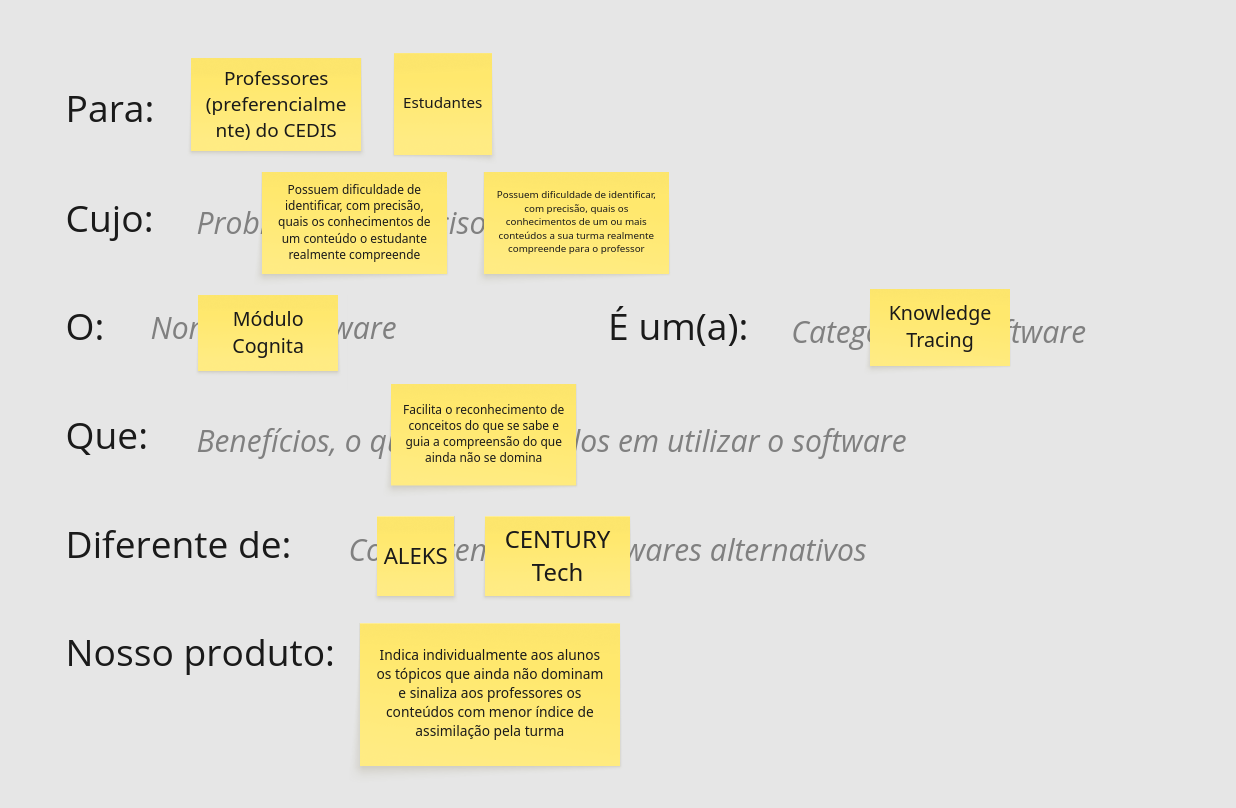
\includegraphics[width=\textwidth]{figuras/visaoProduto.png}
\legend{Fonte: Elaborado pelos autores.}
\end{figure}

Consolidando os elementos sintetizados na Figura~\ref{fig:visao-produto} no formato canônico de declaração preconizado por \citeonline{caroli_lean_2018}, a visão do produto do módulo Cognita é formalizada nos seguintes termos:

\begin{quote}
\textbf{Para} professores (preferencialmente do Ecossistema CEDIS) e estudantes, \textbf{cujo} desafio reside na dificuldade de identificar, com precisão, quais conhecimentos de um conteúdo o estudante realmente compreende e quais conhecimentos de um ou mais conteúdos a turma efetivamente assimilou, \textbf{o} Módulo Cognita \textbf{é um} módulo de \textit{Knowledge Tracing} \textbf{que} facilita o reconhecimento de conceitos do que já se sabe e guia a compreensão do que ainda não se domina. \textbf{Diferente de} plataformas alternativas como ALEKS e CENTURY Tech, \textbf{nosso produto} indica individualmente aos alunos os tópicos que ainda não dominam e sinaliza aos professores os conteúdos com menor índice de assimilação pela turma.
\end{quote}

Essa visão define duas diretrizes para os requisitos. A primeira é o ciclo duplo de \textit{feedback}: no nível individual, o Cognita apoia a autorregulação do estudante, apontando os conceitos que ele ainda não domina; no nível coletivo, apoia as decisões pedagógicas do professor, destacando as dificuldades da turma sem depender apenas de médias de acerto. A segunda é o posicionamento do módulo em relação às plataformas adaptativas tomadas como referência na \textit{Lean Inception}: o \textbf{ALEKS} e a \textbf{CENTURY Tech}.

\subsubsection{Análise das Alternativas: ALEKS e CENTURY Tech}
\label{subsubsec:analise-alternativas}

O \textbf{ALEKS}\footnote{Disponível em \url{https://www.aleks.com}} (\textit{Assessment and LEarning in Knowledge Spaces}) é um sistema de avaliação e tutoria fundamentado na Teoria de Espaços de Conhecimento (\textit{Knowledge Space Theory}, KST) \cite{falmagne_learning_2011}. Nessa teoria, um domínio curricular é modelado como um conjunto de conceitos interdependentes, e o estado de conhecimento do estudante corresponde ao subconjunto de conceitos que ele domina. Por meio de avaliações adaptativas, o sistema seleciona questões para localizar esse estado e indica tanto o que o estudante já domina quanto o que ele está pronto para aprender a seguir. O ALEKS, contudo, opera sobre o seu próprio catálogo de cursos e questões.

A \textbf{CENTURY Tech}\footnote{Disponível em \url{https://www.century.tech}} é uma plataforma comercial de ensino adaptativo organizada em torno de microaulas denominadas \textit{nuggets}, que combinam conteúdo e questões avaliativas. A partir das respostas dos estudantes, a plataforma recomenda ao aluno os tópicos que deve reforçar e oferece ao docente um painel com a situação da turma e de cada estudante. Assim como o ALEKS, opera sobre os seus próprios conteúdos.

A Tabela~\ref{tab:comparativo-alternativas} sintetiza a comparação entre o ALEKS, a CENTURY Tech e o módulo Cognita, evidenciando como o estudo dessas duas ferramentas orientou a proposta de valor do produto.

\begin{table}[htb]
\caption{Comparativo entre as plataformas estudadas (ALEKS e CENTURY Tech) e o módulo Cognita}
\label{tab:comparativo-alternativas}
\centering
\begin{tabularx}{\textwidth}{>{\raggedright\arraybackslash}p{3.0cm}>{\raggedright\arraybackslash}X>{\raggedright\arraybackslash}X>{\raggedright\arraybackslash}X}
\hline
\textbf{Critério} & \textbf{ALEKS} & \textbf{CENTURY Tech} & \textbf{Módulo Cognita} \\
\hline
\textbf{Abordagem de diagnóstico} & Avaliação adaptativa baseada em \textit{Knowledge Space Theory} (KST) e grafos de pré-requisitos. & Modelos contínuos de IA e rastreamento de desempenho sobre microaulas (\textit{nuggets}). & \textit{Knowledge Tracing} aplicado a eventos e respostas de múltiplas fontes do Ecossistema CEDIS. \\
\hline
\textbf{Retorno ao estudante} & Mapa visual setorial (\textit{ALEKS Pie}) indicando tópicos dominados e prontos para estudo. & Trilha personalizada destacando conteúdos de revisão imediata e de avanço. & Indicação individualizada dos conceitos e tópicos que o aluno ainda não domina. \\
\hline
\textbf{Retorno ao professor} & Relatórios de progresso curricular e domínio por tópico. & Painel com a situação da turma e de cada estudante. & Sinalização dos conceitos e conteúdos com menor índice de absorção pela turma. \\
\hline
\textbf{Acoplamento e conteúdo} & Opera sobre o catálogo de cursos e questões da própria plataforma. & Opera sobre os \textit{nuggets} da própria plataforma. & Módulo nativo acoplado ao Ecossistema CEDIS; opera sobre mapas e \textit{decks} criados pelos docentes. \\
\hline
\textbf{Privacidade e governança} & Dados mantidos pelo fornecedor da plataforma. & Dados mantidos pelo fornecedor da plataforma. & Arquitetura \textit{LGPD-first} e \textit{Privacy by Design}, integrada ao consentimento do Learning Passport. \\
\hline
\end{tabularx}
\legend{Fonte: Elaborado pelos autores.}
\end{table}

Dessa forma, enquanto o ALEKS inspira a representação estruturada do domínio conceitual e a CENTURY Tech referencia a entrega simultânea de diagnósticos acionáveis para estudantes e professores, o módulo Cognita diferencia-se por transpor essas capacidades para a arquitetura distribuída do Ecossistema CEDIS. Em vez de exigir que docentes e alunos migrem para uma ferramenta externa, o Cognita aproveita os \textit{decks} publicados no Deck Manager, as respostas coletadas em sala pelo CEDIS Slides, a estruturação semântica do Concept Studio e do Atlas do Conhecimento e a gestão de identidade consentida do Learning Passport.

\subsubsection{Delimitação de Escopo: É/Não é/Faz/Não faz}
\label{subsubsec:e-nao-e-faz-nao-faz}

Em complemento à Declaração de Visão do Produto, executou-se a segunda dinâmica da \textit{Lean Inception}: a matriz \textbf{É/Não é/Faz/Não faz} \cite{caroli_lean_2018}. Em projetos de engenharia de software que combinam análise de dados educacionais e inteligência artificial, é frequente o surgimento de ambiguidades acerca da autonomia decisória do algoritmo, das fronteiras arquiteturais do componente e das implicações éticas de privacidade. Essa atividade busca eliminar tais interpretações divergentes ao confrontar explicitamente as classificações positivas (identidade e capacidades funcionais do sistema) com as restrições negativas (o que o sistema não representa e as ações que estão expressamente vedadas ou fora de seu escopo). A Figura~\ref{fig:detalhes-modulo} apresenta o artefato visual resultante dessa etapa.

\begin{figure}[htb]
\caption{Artefato da atividade ``É/Não é/Faz/Não faz'' na \textit{Lean Inception}}
\label{fig:detalhes-modulo}
\centering
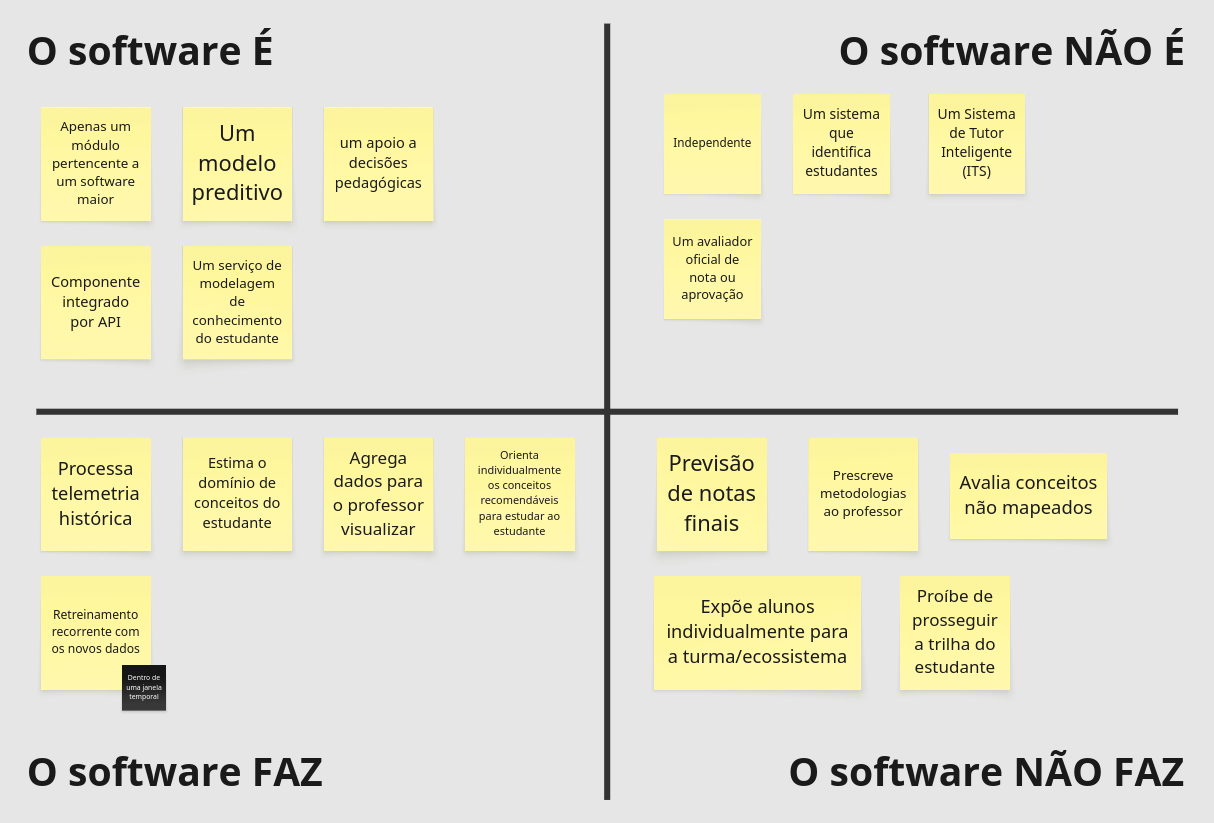
\includegraphics[width=\textwidth]{figuras/detalhesModulo.png}
\legend{Fonte: Elaborado pelos autores.}
\end{figure}

O desdobramento analítico de cada quadrante da Figura~\ref{fig:detalhes-modulo} estabelece premissas técnicas, pedagógicas e regulatórias que condicionam diretamente os requisitos funcionais e não funcionais do módulo Cognita:

\begin{enumerate}
    \item \textbf{O software É (Natureza e papel arquitetural):}
    \begin{itemize}
        \item \textbf{Apenas um módulo pertencente a um software maior:} O Cognita não constitui um ambiente virtual de aprendizagem autônomo, mas sim um módulo analítico especializado concebido para operar no interior do Ecossistema CEDIS, acoplando-se nativamente à camada do CEDIS Learning Analytics.
        \item \textbf{Componente integrado por API:} Sua comunicação com os demais produtos do ecossistema (Deck Manager, CEDIS Slides, Concept Studio, Atlas do Conhecimento e Learning Passport) ocorre de maneira estritamente desacoplada, mediada por contratos explícitos de API e pelos protocolos de segurança e autenticidade já padronizados na plataforma (OAuth2, OIDC e HMAC).
        \item \textbf{Um modelo preditivo e um serviço de modelagem de conhecimento do estudante:} No plano computacional, a essência do módulo reside na manutenção e atualização contínua de uma representação probabilística do estado cognitivo latente de cada aluno, inferindo o grau de domínio sobre conceitos específicos a partir de evidências observáveis de interação.
        \item \textbf{Um apoio a decisões pedagógicas:} No plano educacional, o módulo funciona como um sistema de apoio à decisão (\textit{Decision Support System}), que subsidia tanto a autorregulação do estudo pelo aluno quanto o replanejamento didático pelo docente.
    \end{itemize}

    \item \textbf{O software NÃO É (Restrições de identidade do sistema):}
    \begin{itemize}
        \item \textbf{Independente:} O Cognita não opera de forma isolada (\textit{standalone}), dependendo estruturalmente da coleta de respostas no CEDIS Slides, da gestão operacional do Deck Manager e do mapeamento semântico de conceitos realizado no Concept Studio e no Atlas do Conhecimento.
        \item \textbf{Um sistema que identifica estudantes:} Em conformidade estrita com os princípios de \textit{Privacy by Design} \cite{cavoukian_privacy_2009} e a diretriz \textit{LGPD-first} do ecossistema, o módulo não atua como ferramenta de identificação civil ou vigilância individualizada. A associação longitudinal de interações apoia-se exclusivamente em identificadores pseudonimizados de passaportes com consentimento explícito (\textit{opt-in}), gerido pelo CEDIS Learning Passport.
        \item \textbf{Um Sistema de Tutor Inteligente (\textit{Intelligent Tutoring System}, ITS):} Diferentemente de um ITS completo, que controla o fluxo instrucional passo a passo, ministra explicações teóricas automatizadas e gera novos problemas em tempo real, o Cognita atua especificamente na camada diagnóstica de rastreamento de conhecimento (\textit{Knowledge Tracing}), delegando a autoria e a apresentação de conteúdos aos produtos existentes do ecossistema.
        \item \textbf{Um avaliador oficial de nota ou aprovação:} O módulo possui caráter estritamente formativo e diagnóstico, não substituindo instrumentos somativos formais nem detendo autoridade acadêmica para atribuir menções ou aprovar/reprovar discentes.
    \end{itemize}

    \item \textbf{O software FAZ (Responsabilidades funcionais e analíticas):}
    \begin{itemize}
        \item \textbf{Processa telemetria histórica:} O módulo consome e reconcilia séries temporais de eventos de aprendizagem e respostas persistidas (vinculadas por entidades como \textit{LearningAnalyticsIngestLink} e \textit{QuestionActivityMap}), transformando registros operacionais brutos em vetores de atributos (\textit{features}) cronologicamente ordenados.
        \item \textbf{Estima o domínio de conceitos do estudante:} Aplicando algoritmos de \textit{Knowledge Tracing} sobre a sequência histórica de acertos, erros e interações, o serviço calcula a probabilidade atualizada de domínio de cada conceito mapeado para o estudante.
        \item \textbf{Orienta individualmente os conceitos recomendáveis para estudo:} A partir das probabilidades inferidas, identifica as lacunas conceituais mais críticas do aluno e disponibiliza indicações individualizadas sobre quais tópicos demandam revisão prioritária.
        \item \textbf{Agrega dados para o professor visualizar:} Consolida as estimativas individuais de domínio em indicadores coletivos por turma e por conceito, respeitando regras de supressão e \textit{k}-anonimato, permitindo ao docente visualizar com clareza os conteúdos com menor índice de absorção.
        \item \textbf{Retreinamento recorrente com os novos dados (dentro de uma janela temporal):} Para evitar a degradação preditiva decorrente de mudanças no perfil das turmas ou na estrutura dos materiais (\textit{concept drift}), o \textit{pipeline} do módulo executa ciclos periódicos de retreinamento do modelo dentro de janelas temporais predefinidas, incorporando os novos lotes de interações consolidadas no ecossistema.
    \end{itemize}

    \item \textbf{O software NÃO FAZ (Fronteiras negativas de comportamento):}
    \begin{itemize}
        \item \textbf{Previsão de notas finais:} O escopo preditivo restringe-se à estimativa de domínio por conceito no curto e médio prazo, não realizando regressão ou classificação voltada a prever a nota ou menção final do estudante na disciplina.
        \item \textbf{Prescreve metodologias ao professor:} Embora sinalize quais conceitos apresentam déficit de absorção na turma, o Cognita não impõe nem prescreve qual abordagem pedagógica ou didática o docente deve adotar em sala de aula, preservando integralmente a autonomia e o julgamento profissional do educador.
        \item \textbf{Avalia conceitos não mapeados:} A inferência de domínio exige que as questões e atividades respondidas possuam vínculo explícito com conceitos cadastrados no banco semântico do ecossistema (via \textit{QuestionActivityMap}); interações em atividades sem conceitos previamente associados não são objeto de adivinhação ou inferência arbitrária pelo modelo.
        \item \textbf{Expõe alunos individualmente para a turma ou ecossistema:} É expressamente vedada qualquer funcionalidade de ranqueamento público, comparação nominal ostensiva ou exposição das vulnerabilidades cognitivas de um estudante para seus pares ou para terceiros não autorizados.
        \item \textbf{Proíbe de prosseguir a trilha do estudante:} As recomendações geradas pelo Cognita têm natureza consultiva e orientadora (\textit{soft guidance}); o módulo não aplica bloqueios rígidos (\textit{hard gating}) que impeçam o estudante de navegar livremente pelos \textit{decks} do CEDIS Slides ou explorar novos nós no Atlas do Conhecimento.
    \end{itemize}
\end{enumerate}

\subsection{Personas}
\label{subsec:personas}

Na metodologia \textit{Lean Inception}, a modelagem de personas tem por finalidade humanizar e tangibilizar os segmentos de usuários identificados na Visão do Produto, evitando que a especificação de requisitos se baseie em suposições genéricas sobre um ``usuário médio'' \cite{caroli_lean_2018}. Cada persona sintetiza um arquétipo realista de ator que interage com o Ecossistema CEDIS, estruturado em quatro dimensões: identificação representativa (\textbf{Nome e Imagem}), contexto demográfico e acadêmico (\textbf{Perfil}), traços comportamentais e cognitivos (\textbf{Características Intrínsecas}) e demandas diretas em relação à solução (\textbf{Necessidades}). Ao todo, foram mapeadas três personas complementares para orientar as histórias de usuário do módulo Cognita, sendo todas elas submetidas à revisão e validação direta junto ao cliente do projeto, de modo a assegurar sua aderência à realidade operacional e pedagógica do ecossistema.

\subsubsection{Persona 1: Estudante de Engenharia de Software (João Guilherme / Marina Silva)}
\label{subsubsec:persona-1}

A primeira persona, personificada pelos perfis equivalentes de \textbf{João Guilherme} e \textbf{Marina Silva}, representa o público-alvo primário da camada de retorno individual do Cognita: o discente de graduação inserido em disciplinas técnicas de alta carga conceitual na Universidade de Brasília (UnB). A Figura~\ref{fig:persona-1} apresenta o quadro construído para essa persona durante a dinâmica colaborativa.

\begin{figure}[htb]
\caption{Artefato da Persona 1 (Estudante de Engenharia de Software) na \textit{Lean Inception}}
\label{fig:persona-1}
\centering
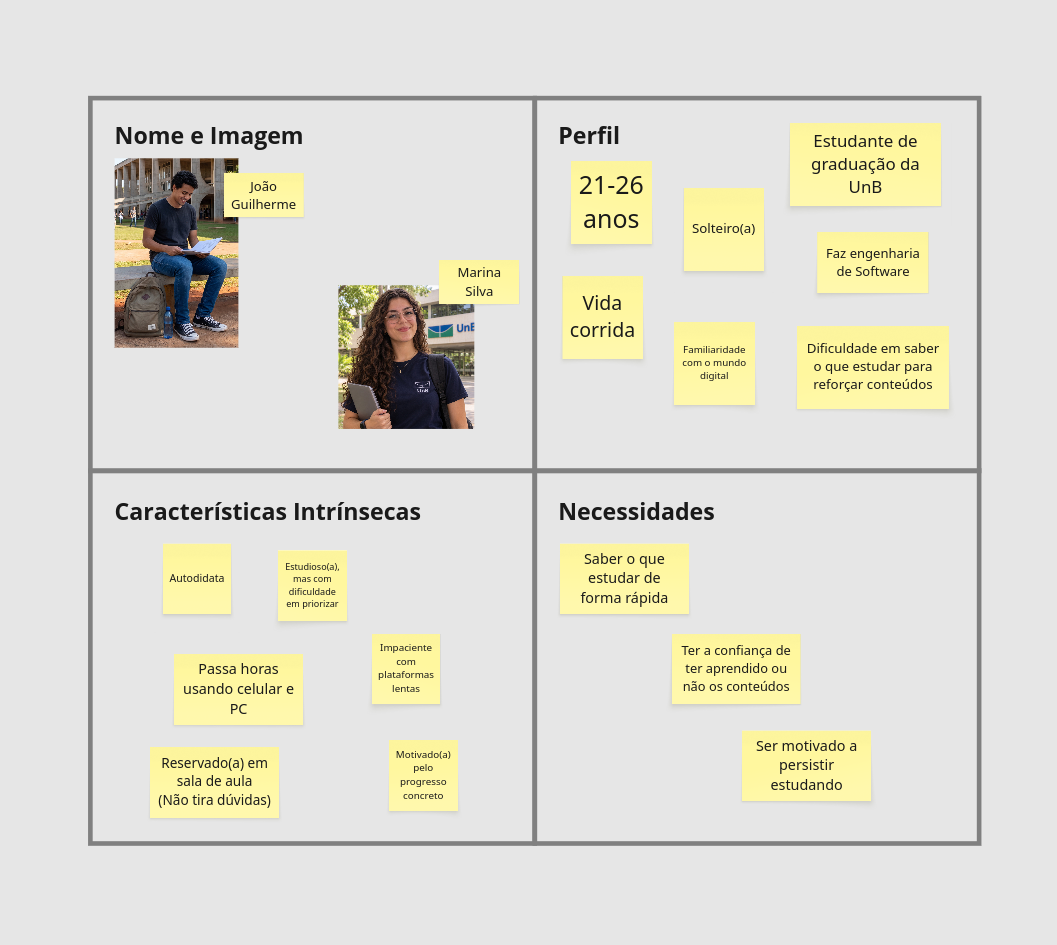
\includegraphics[width=\textwidth]{figuras/persona1.png}
\legend{Fonte: Elaborado pelos autores.}
\end{figure}

A análise detalhada dos quatro quadrantes da Figura~\ref{fig:persona-1} revela como o contexto cotidiano e os hábitos de estudo desse perfil condicionam tanto os requisitos funcionais de recomendação quanto os atributos de qualidade (requisitos não funcionais) do módulo Cognita:

\begin{enumerate}
    \item \textbf{Perfil (Contexto demográfico, acadêmico e dor central):}
    \begin{itemize}
        \item \textbf{Estudante de graduação da UnB em Engenharia de Software:} Trata-se de um estudante em fase intermediária ou avançada do curso, submetido a disciplinas cujos conteúdos possuem forte encadeamento de pré-requisitos lógicos e arquiteturais (como estruturas de dados, arquitetura de software, bancos de dados e aprendizagem de máquina).
        \item \textbf{Vida corrida:} A rotina acadêmica intensa, frequentemente conciliada com estágios, iniciação científica, projetos integradores e deslocamentos, deixa pouco tempo livre para o estudo extraclasse.
        \item \textbf{Familiaridade com o mundo digital:} Por atuar na área de tecnologia, possui alta proficiência no uso de aplicações web e móveis, esperando interfaces intuitivas, modernas e sem fricção operacional.
        \item \textbf{Dificuldade em saber o que estudar para reforçar conteúdos:} Diante de ementas extensas e múltiplos \textit{decks} de aula, o estudante não consegue isolar com precisão qual conceito de base não foi compreendido quando erra um exercício mais complexo, resultando em perda de tempo com revisões amplas e pouco efetivas.
    \end{itemize}

    \item \textbf{Características Intrínsecas (Comportamento e atitude de aprendizagem):}
    \begin{itemize}
        \item \textbf{Autodidata, estudioso(a), mas com dificuldade em priorizar:} O aluno possui iniciativa e disposição para buscar o conhecimento por conta própria nos materiais do Ecossistema CEDIS (como o Atlas do Conhecimento e os \textit{decks} do CEDIS Slides). Entretanto, sem um diagnóstico externo calibrado, tende a dispersar esforço estudando tópicos que já domina ou tentando avançar sem consolidar lacunas anteriores.
        \item \textbf{Reservado(a) em sala de aula (não tira dúvidas):} Por timidez, receio de exposição perante a turma ou pela própria percepção tardia da dúvida, esse estudante raramente interrompe a aula expositiva para questionar o professor. Esse traço comportamental evidencia uma falha crítica do ensino tradicional presencial e justifica diretamente dois pilares do Cognita: o fornecimento de um canal privado e não estigmatizante de diagnóstico ao aluno e a sinalização agregada ao docente sobre dúvidas silenciosas da turma.
        \item \textbf{Passa horas usando celular e PC e é impaciente com plataformas lentas:} O hábito de alternar entre o dispositivo móvel (utilizado para responder atividades em tempo real no CEDIS Slides durante a aula) e o computador pessoal (utilizado em sessões de estudo focado) exige que o ecossistema e o módulo analítico apresentem alta responsividade e baixa latência no processamento e exibição das estimativas de domínio.
        \item \textbf{Motivado(a) pelo progresso concreto:} Perceber a própria evolução, isto é, ver que um conceito antes deficitário passou ao estado de domínio após a prática, estimula o engajamento contínuo desse perfil.
    \end{itemize}

    \item \textbf{Necessidades (Objetivos de valor esperados do módulo Cognita):}
    \begin{itemize}
        \item \textbf{Saber o que estudar de forma rápida:} Dada sua rotina sobrecarregada e a dificuldade de priorização, a persona necessita que o sistema traduza imediatamente seu histórico de interações em um apontamento direto dos conceitos prioritários que requerem reforço, eliminando o tempo gasto procurando o que revisar.
        \item \textbf{Ter a confiança de ter aprendido ou não os conteúdos:} Mais do que visualizar o gabarito de uma questão isolada, o estudante precisa de um indicador confiável, fundamentado pelo modelo de \textit{Knowledge Tracing}, que valide se sua compreensão do conceito subjacente é sólida ou se o acerto pontual ainda mascara uma fragilidade cognitiva.
        \item \textbf{Ser motivado a persistir estudando:} O retorno visual sobre a evolução de seu estado de conhecimento ao longo do semestre deve reforçar sua autoeficácia acadêmica, estimulando a persistência na resolução de atividades e no fechamento progressivo das lacunas identificadas.
    \end{itemize}
\end{enumerate}

\subsubsection{Persona 2: Docente da UnB Vinculado ao CEDIS (Marcelo Andrade / Patrícia Silva)}
\label{subsubsec:persona-2}

A segunda persona, representada pelos arquétipos equivalentes de \textbf{Marcelo Andrade} e \textbf{Patrícia Silva}, personifica o usuário primário da camada de diagnóstico coletivo e apoio à decisão pedagógica do módulo Cognita: o professor universitário que produz materiais didáticos, ministra aulas apoiadas pelo Ecossistema CEDIS e busca aprimorar continuamente o aprendizado de suas turmas. A Figura~\ref{fig:persona-2} apresenta o artefato visual elaborado e validado para esse perfil.

\begin{figure}[htb]
\caption{Artefato da Persona 2 (Docente da UnB vinculado ao CEDIS) na \textit{Lean Inception}}
\label{fig:persona-2}
\centering
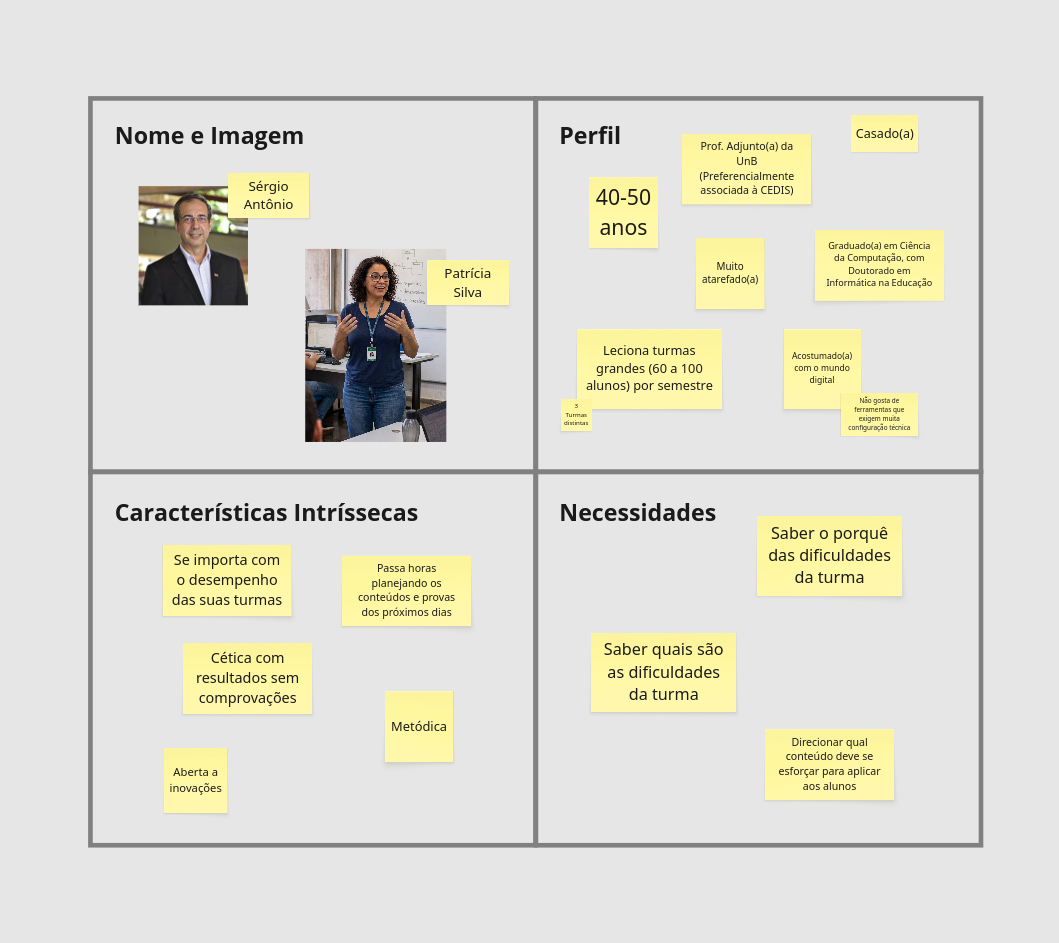
\includegraphics[width=\textwidth]{figuras/persona2.png}
\legend{Fonte: Elaborado pelos autores.}
\end{figure}

O exame pormenorizado dos quatro quadrantes da Figura~\ref{fig:persona-2} explicita as restrições operacionais da docência universitária em larga escala e fundamenta os requisitos analíticos e de usabilidade voltados ao professor:

\begin{enumerate}
    \item \textbf{Perfil (Contexto profissional, carga docente e relação com tecnologia):}
    \begin{itemize}
        \item \textbf{Professor(a) Adjunto(a) da UnB, preferencialmente associado(a) ao CEDIS:} Trata-se de um docente pesquisador que concilia atividades de ensino de graduação e pós-graduação, orientação de alunos, extensão e gestão universitária, resultando em uma rotina altamente sobrecarregada (\textbf{muito atarefado/a}).
        \item \textbf{Graduado(a) em Ciência da Computação, com Doutorado em Informática na Educação:} Possui formação técnica e pedagógica, compreendendo profundamente tanto a estrutura lógica dos conteúdos computacionais quanto os processos cognitivos de ensino-aprendizagem mediados por tecnologia.
        \item \textbf{Leciona turmas grandes (60 a 100 alunos) em 3 turmas distintas por semestre:} Responsável por acompanhar entre 180 e 300 estudantes simultaneamente a cada período letivo, o docente enfrenta uma limitação de escala para diagnosticar manualmente o progresso individual ou perceber lacunas silenciosas antes da aplicação das provas formais, especialmente diante de estudantes reservados como os retratados na Persona~1.
        \item \textbf{Acostumado(a) com o mundo digital, mas avesso(a) a ferramentas que exigem muita configuração técnica:} Embora utilize cotidianamente os produtos do Ecossistema CEDIS (Deck Manager, CEDIS Slides e Concept Studio), o docente não dispõe de tempo para parametrizar modelos complexos ou exportar e cruzar planilhas manualmente. Isso impõe que o Cognita opere de forma transparente e automatizada sobre os vínculos entre \textit{decks}, atividades e conceitos já cadastrados no fluxo normal de preparação de aula.
    \end{itemize}

    \item \textbf{Características Intrínsecas (Postura pedagógica e rigor analítico):}
    \begin{itemize}
        \item \textbf{Se importa com o desempenho das suas turmas e passa horas planejando conteúdos e provas:} O docente demonstra elevado comprometimento com a qualidade didática, investindo tempo expressivo na curadoria de \textit{decks} interativos e na elaboração de avaliações coerentes com os objetivos de aprendizagem da disciplina.
        \item \textbf{Metódico(a) e aberto(a) a inovações:} Busca sistematizar suas aulas em etapas estruturadas (como mapas conceituais e sequências didáticas) e adota proativamente novas tecnologias educacionais quando estas demonstram utilidade prática em sala de aula.
        \item \textbf{Cético(a) com resultados sem comprovações:} Devido à sua formação científica em Computação e Informática na Educação, esse perfil rejeita métricas superficiais de vaidade (como mera contagem de acessos ou visualizações de slides) e desconfia de alertas opacos sem lastro empírico. Para conquistar a confiança dessa persona, o diagnóstico do Cognita precisa ser rastreável às interações reais nas atividades e fundamentado em uma modelagem consistente de \textit{Knowledge Tracing}.
    \end{itemize}

    \item \textbf{Necessidades (Demandas de suporte à decisão pedagógica):}
    \begin{itemize}
        \item \textbf{Saber quais são as dificuldades da turma:} O docente necessita de uma visão consolidada e imediata que aponte, dentre todos os conceitos ministrados em um conjunto de \textit{decks} ou unidades curriculares, exatamente aqueles que apresentam o menor índice de absorção coletiva.
        \item \textbf{Saber o porquê das dificuldades da turma:} Além de identificar o tópico problemático, o professor precisa compreender a origem estrutural da defasagem, isto é, distinguir se o baixo desempenho decorre da não absorção de um conceito pré-requisito anterior no mapa conceitual ou da complexidade intrínseca de um conceito recém-introduzido.
        \item \textbf{Direcionar qual conteúdo deve se esforçar para aplicar aos alunos:} Com base em evidências diagnósticas precisas por turma, o docente busca otimizar seu escasso tempo de planejamento e de aula presencial, direcionando revisões focadas, exemplos adicionais ou novas atividades interativas especificamente para os conceitos críticos antes das avaliações somativas.
    \end{itemize}
\end{enumerate}

\subsubsection{Persona 3: Estudante Autônomo em Profissionalização (Ricardo Gomes / Letícia Carvalho)}
\label{subsubsec:persona-3}

A terceira persona, representada pelos perfis equivalentes de \textbf{Ricardo Gomes} e \textbf{Letícia Carvalho}, contempla um segmento estratégico que transcende as fronteiras da sala de aula formal: o estudante externo e autônomo que utiliza os recursos abertos do Ecossistema CEDIS (como \textit{decks} públicos, o Concept Studio e o Atlas do Conhecimento) com foco em capacitação contínua e inserção ou progressão no mercado de Tecnologia da Informação (TI). A Figura~\ref{fig:persona-3} ilustra o quadro consolidado e validado para essa persona.

\begin{figure}[htb]
\caption{Artefato da Persona 3 (Estudante autônomo em profissionalização) na \textit{Lean Inception}}
\label{fig:persona-3}
\centering
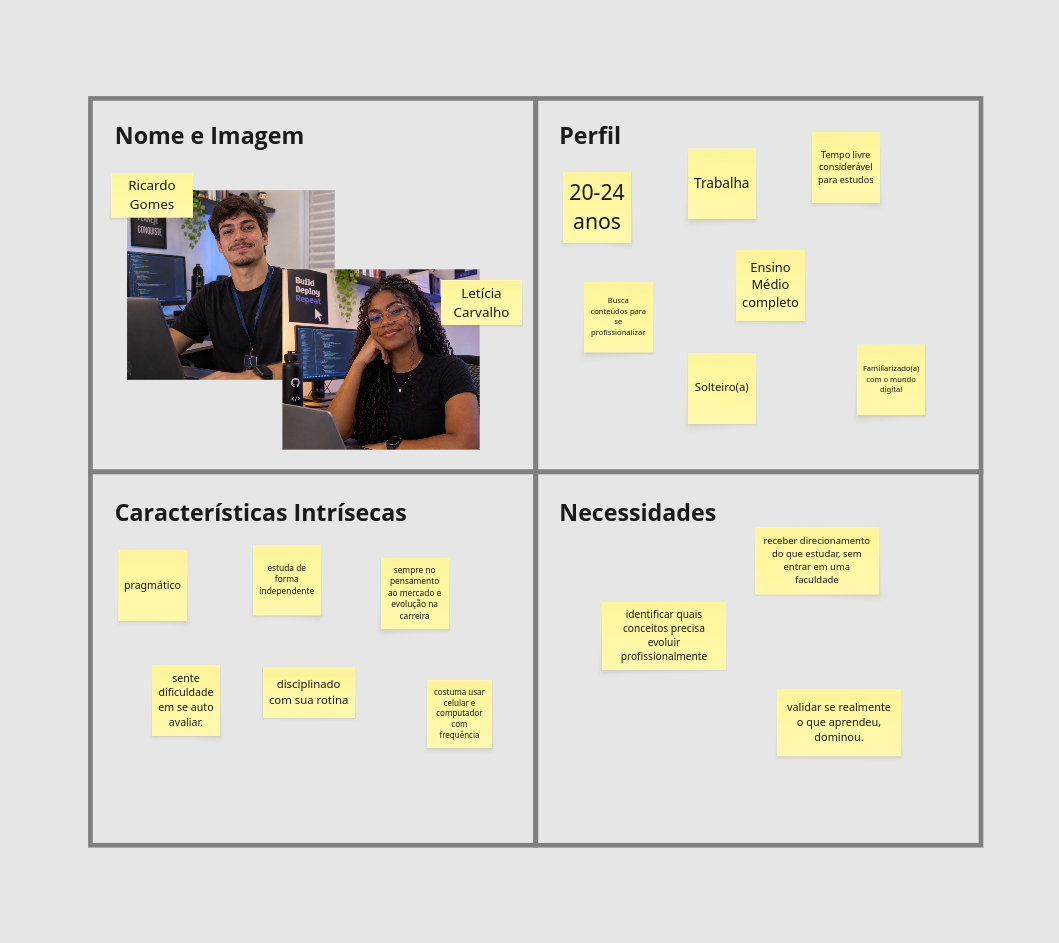
\includegraphics[width=\textwidth]{figuras/persona3.png}
\legend{Fonte: Elaborado pelos autores.}
\end{figure}

O detalhamento dos quatro quadrantes da Figura~\ref{fig:persona-3} evidencia como as demandas de um aprendiz independente complementam os requisitos do módulo Cognita:

\begin{enumerate}
    \item \textbf{Perfil (Contexto socioeconômico, formativo e disponibilidade):}
    \begin{itemize}
        \item \textbf{Jovem profissional de TI com Ensino Médio completo, que trabalha na área:} Diferentemente da Persona~1, este usuário já atua operacionalmente no mercado de tecnologia sem estar matriculado em um curso superior formal. Sua formação técnica deu-se por vias práticas, cursos livres e documentação online.
        \item \textbf{Busca conteúdos para se profissionalizar e dispõe de tempo livre considerável para estudos:} Por não possuir a grade horária rígida de uma graduação presencial e manter rotina pessoal flexível, dedica janelas regulares durante a semana para consumir materiais estruturados que elevem sua qualificação técnica.
        \item \textbf{Familiarizado(a) com o mundo digital:} Apresenta fluência natural na navegação por plataformas web e ecossistemas digitais de aprendizagem.
    \end{itemize}

    \item \textbf{Características Intrínsecas (Autonomia, pragmatismo e limitação metacognitiva):}
    \begin{itemize}
        \item \textbf{Pragmático(a) e sempre voltado(a) ao mercado e à evolução na carreira:} Prioriza conhecimentos que possuam aplicabilidade clara em seu cotidiano de trabalho. Entretanto, o aprendizado puramente prático frequentemente oculta lacunas em fundamentos teóricos de computação e engenharia de software que limitam sua progressão para níveis técnicos mais complexos.
        \item \textbf{Estuda de forma independente e é disciplinado(a) com sua rotina:} Mantém constância de estudo por conta própria e utiliza celular e computador com frequência, mas realiza toda a sua jornada sem o acompanhamento de um professor ou monitor para orientar seus passos.
        \item \textbf{Sente dificuldade em se autoavaliar:} Na ausência de provas acadêmicas formais e de \textit{feedback} docente, esse perfil enfrenta forte incerteza metacognitiva, muitas vezes acreditando dominar um tópico por conseguir reproduzir um tutorial prático, ou sentindo-se inseguro sobre a solidez de sua base conceitual.
    \end{itemize}

    \item \textbf{Necessidades (Objetivos de direcionamento e validação autônoma):}
    \begin{itemize}
        \item \textbf{Receber direcionamento do que estudar, sem entrar em uma faculdade:} Necessita que o próprio ecossistema atue como um guia estruturado, indicando a sequência lógica de conceitos a serem reforçados sem depender de uma grade curricular universitária tradicional.
        \item \textbf{Identificar quais conceitos precisa evoluir profissionalmente:} Precisa que o módulo Cognita diagnostique com precisão quais fundamentos e pré-requisitos teóricos ainda estão defasados em sua formação prática, permitindo um estudo focado ao fechamento dessas lacunas.
        \item \textbf{Validar se realmente dominou o que aprendeu:} Demanda um indicador objetivo e confiável, provido pelas estimativas de \textit{Knowledge Tracing} vinculadas ao seu histórico no CEDIS Learning Passport, que ateste o efetivo domínio dos conceitos estudados.
    \end{itemize}
\end{enumerate}

Em conjunto, as três personas cobrem os fluxos de valor do Cognita. A \textbf{Persona~1} fundamenta os requisitos de diagnóstico rápido e de priorização para o estudante universitário com pouco tempo; a \textbf{Persona~2}, a agregação por turma e a rastreabilidade dos diagnósticos para o docente de turmas grandes; e a \textbf{Persona~3}, o uso do diagnóstico individual como ferramenta de autoavaliação para estudantes fora do ambiente acadêmico formal.

\subsection{Jornadas do Usuário}
\label{subsec:jornadas-usuario}

Uma vez estabelecidas e validadas as três personas do projeto, conduziu-se a atividade de mapeamento das \textbf{Jornadas do Usuário} da \textit{Lean Inception} \cite{caroli_lean_2018}. O objetivo desse artefato é descrever a sequência cronológica de etapas que cada persona percorre desde o contexto inicial de uso do Ecossistema CEDIS e a emergência de sua dor informacional até o atingimento de seu objetivo pedagógico ou profissional, explicitando os pontos de contato (\textit{touchpoints}) em que o módulo Cognita intervém para gerar valor.

\subsubsection{Jornada da Persona 1: Estudante de Engenharia de Software (João Guilherme / Marina Silva)}
\label{subsubsec:jornada-persona-1}

A jornada da primeira persona retrata o percurso do estudante de graduação da UnB em uma disciplina presencial apoiada pelos produtos do Ecossistema CEDIS, evidenciando a transição entre a dúvida silenciosa em sala de aula e o estudo direcionado extraclasse. A Figura~\ref{fig:jornada-persona-1} apresenta os oito passos que compõem esse fluxo.

\begin{figure}[htb]
\caption{Artefato da Jornada da Persona 1 (Estudante de Engenharia de Software) na \textit{Lean Inception}}
\label{fig:jornada-persona-1}
\centering
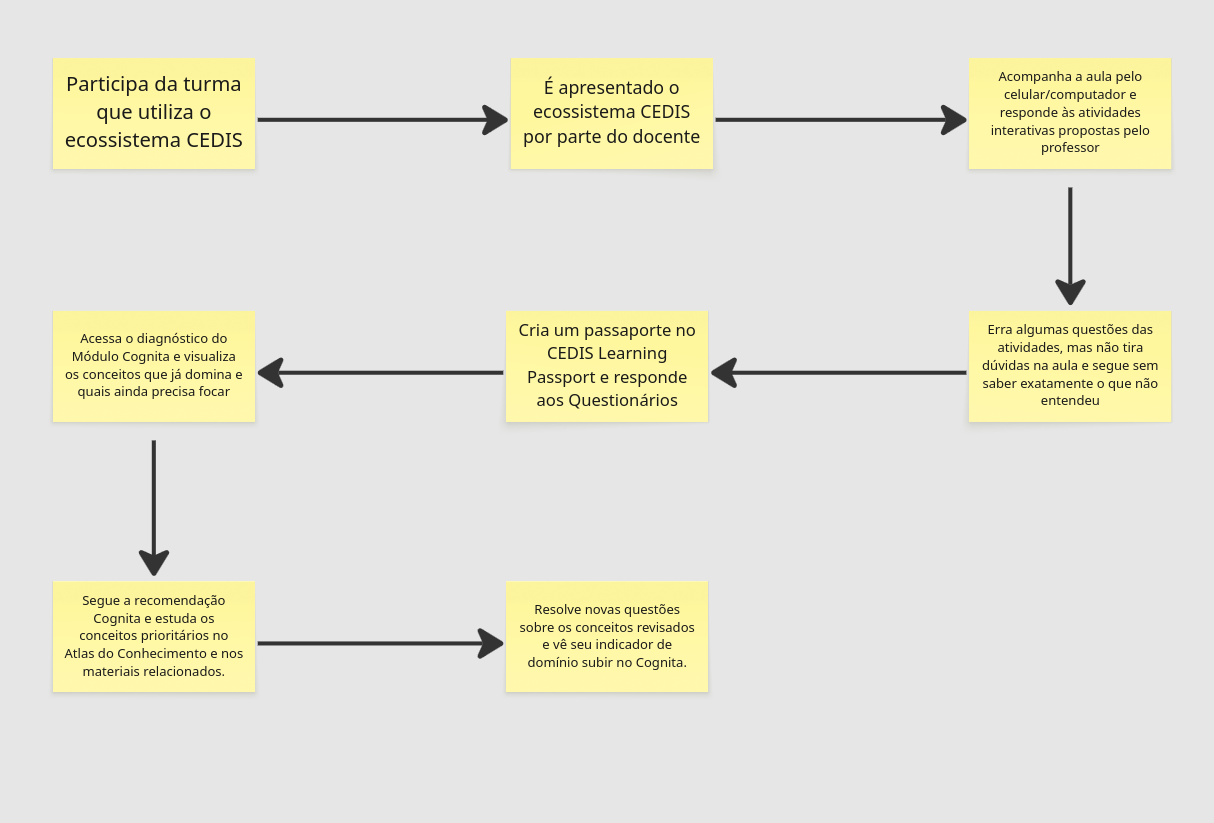
\includegraphics[width=\textwidth]{figuras/persona1Jornada.png}
\legend{Fonte: Elaborado pelos autores.}
\end{figure}

O desdobramento sequencial da Figura~\ref{fig:jornada-persona-1} compreende as seguintes etapas e interações sistêmicas:

\begin{enumerate}
    \item \textbf{Inserção no contexto acadêmico:} O estudante matricula-se e participa de uma turma de graduação na UnB cujo docente adota o Ecossistema CEDIS como infraestrutura de apoio didático;
    \item \textbf{Apresentação da plataforma:} No início do período letivo, o docente apresenta aos alunos o funcionamento integrado dos produtos do ecossistema para acompanhamento das aulas e realização de exercícios;
    \item \textbf{Interação síncrona em sala de aula:} Durante a exposição teórica, o estudante acompanha os slides pelo próprio celular ou computador no \textbf{CEDIS Slides} e submete respostas às atividades interativas propostas pelo professor (gerando eventos de telemetria e registros de resposta vinculados aos conceitos via \textit{QuestionActivityMap});
    \item \textbf{Emergência do ponto de dor silencioso:} O aluno erra determinadas questões das atividades, mas, por seu perfil reservado em sala de aula, não interrompe o professor para tirar dúvidas e encerra a aula sem saber exatamente qual conceito fundamental deixou de compreender;
    \item \textbf{Habilitação de identidade persistente e prática individual:} Para acompanhar seu histórico longitudinal de aprendizagem sob controle próprio e em conformidade com a LGPD, o estudante cria seu passaporte no \textbf{CEDIS Learning Passport} e, a partir dele, responde aos questionários individuais do \textbf{Atlas do Conhecimento} sobre os conceitos da aula (estabelecendo a reconciliação via \textit{LearningAnalyticsIngestLink});
    \item \textbf{Diagnóstico individual no Módulo Cognita (Ponto de contato central):} Ao iniciar sua sessão de estudos, o aluno acessa o diagnóstico processado pelo \textbf{Módulo Cognita} e visualiza com clareza a separação entre os conceitos que já domina e aqueles nos quais ainda apresenta baixa estimativa de domínio, calculada a partir das respostas registradas desde a criação do passaporte;
    \item \textbf{Estudo direcionado no ecossistema:} Guiado pela recomendação prioritária do Cognita, que reduz a indecisão sobre o que estudar em sua rotina corrida, o estudante navega diretamente para os conceitos vulneráveis no \textbf{Atlas do Conhecimento} e revisa os materiais didáticos correspondentes;
    \item \textbf{Validação de progresso e reforço motivacional:} Após a revisão, o estudante resolve novas questões associadas aos conceitos estudados e observa a elevação de seu indicador de domínio no Cognita, consolidando sua confiança no aprendizado.
\end{enumerate}

Caso o estudante já possua passaporte antes da aula, suas respostas às atividades em sala de aula (passo 3) também são consideradas pelo Cognita. Por serem realizadas em formato de jogo entre os estudantes, essas atividades fornecem uma evidência menos confiável do que os questionários individuais, o que é refletido no modelo por meio de parâmetros de chute e descuido próprios para essa origem (Seção~\ref{subsubsec:oe4}).

\subsubsection{Jornada da Persona 2: Docente da UnB Vinculado ao CEDIS (Marcelo Andrade / Patrícia Silva)}
\label{subsubsec:jornada-persona-2}

A jornada da segunda persona modela o ciclo de trabalho pedagógico do professor universitário responsável por turmas numerosas, demonstrando como o módulo Cognita preenche a lacuna entre a coleta massiva de respostas em sala e o replanejamento didático fundamentado em evidências. A Figura~\ref{fig:jornada-persona-2} ilustra os seis passos desse fluxo.

\begin{figure}[htb]
\caption{Artefato da Jornada da Persona 2 (Docente da UnB vinculado ao CEDIS) na \textit{Lean Inception}}
\label{fig:jornada-persona-2}
\centering
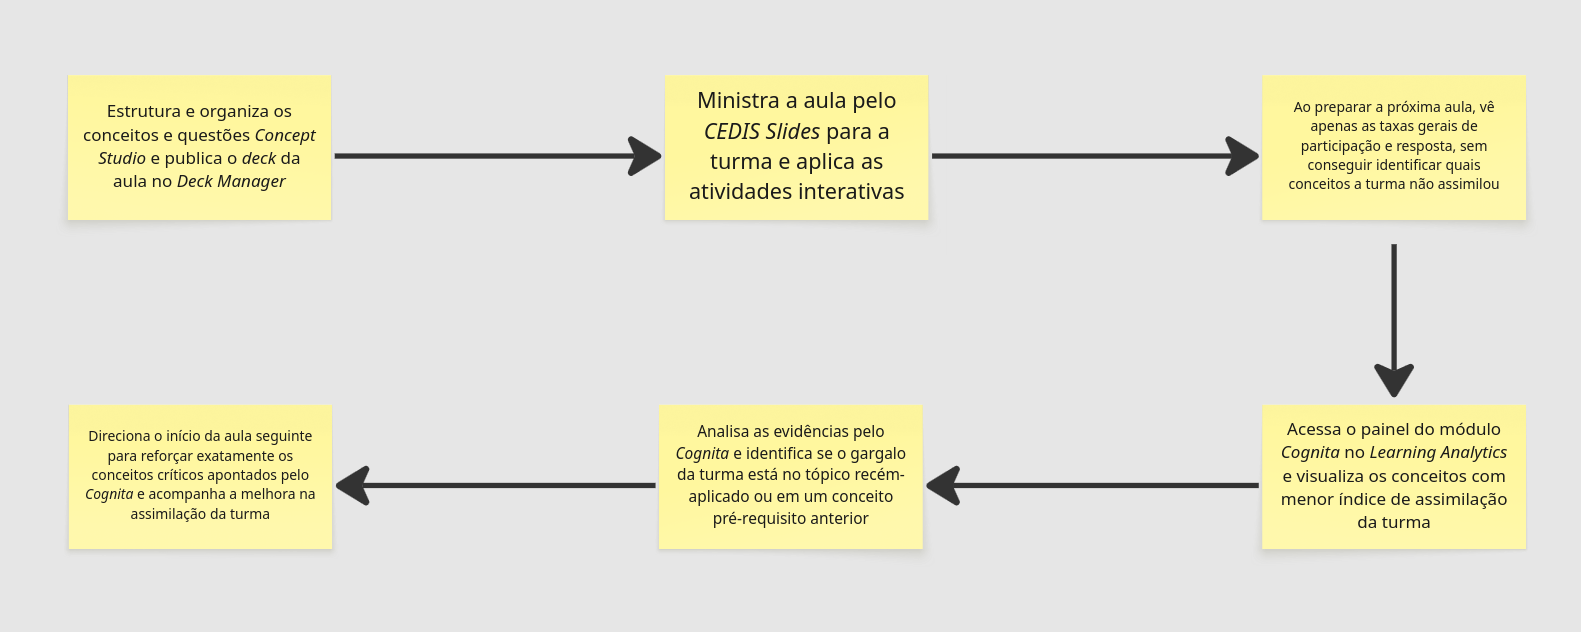
\includegraphics[width=\textwidth]{figuras/persona2Jornada.png}
\legend{Fonte: Elaborado pelos autores.}
\end{figure}

As seis etapas representadas na Figura~\ref{fig:jornada-persona-2} articulam-se da seguinte forma:

\begin{enumerate}
    \item \textbf{Estruturação semântica e publicação do material:} No preparo da disciplina, o docente estrutura e organiza os mapas conceituais e o banco de questões no \textbf{Concept Studio} e publica o \textit{deck} correspondente da aula no \textbf{CEDIS Deck Manager};
    \item \textbf{Mediação em sala e coleta de respostas:} O professor ministra a aula expositiva utilizando o \textbf{CEDIS Slides} para sua turma (de 60 a 100 estudantes) e aplica as atividades interativas ao longo da apresentação;
    \item \textbf{Limitação das métricas puramente descritivas (Ponto de dor):} Ao encerrar o encontro e iniciar o preparo da próxima aula, o docente dispõe apenas de taxas gerais de participação, submissão e distribuição bruta de respostas, sem conseguir identificar com precisão quais conceitos subjacentes a turma efetivamente deixou de assimilar;
    \item \textbf{Consulta ao diagnóstico coletivo no Módulo Cognita (Ponto de contato central):} O professor acessa o painel do \textbf{Módulo Cognita} integrado ao \textbf{CEDIS Learning Analytics} e visualiza, sem necessidade de configurações técnicas adicionais, o ranqueamento dos conceitos com menor índice de absorção pela turma;
    \item \textbf{Análise das possíveis origens das dificuldades da turma:} A partir das evidências consolidadas pelo modelo de \textit{Knowledge Tracing} do Cognita, o docente analisa se o gargalo coletivo reside no tópico recém-introduzido em aula ou na defasagem acumulada em um conceito pré-requisito anterior;
    \item \textbf{Intervenção pedagógica direcionada:} Munido de comprovação empírica sobre as lacunas da turma, o professor direciona o início da aula seguinte para reforçar exatamente os conceitos críticos apontados pelo Cognita e acompanha a evolução subsequente dos indicadores de absorção coletiva.
\end{enumerate}

\subsubsection{Jornada da Persona 3: Estudante Autônomo em Profissionalização (Ricardo Gomes / Letícia Carvalho)}
\label{subsubsec:jornada-persona-3}

A jornada da terceira persona descreve o percurso de aprendizagem autodirigida de um profissional de TI que recorre ao Ecossistema CEDIS para suprir demandas reais do mercado de trabalho sem estar inserido em uma turma universitária formal. A Figura~\ref{fig:jornada-persona-3} apresenta as nove etapas mapeadas para esse cenário.

\begin{figure}[htb]
\caption{Artefato da Jornada da Persona 3 (Estudante autônomo em profissionalização) na \textit{Lean Inception}}
\label{fig:jornada-persona-3}
\centering
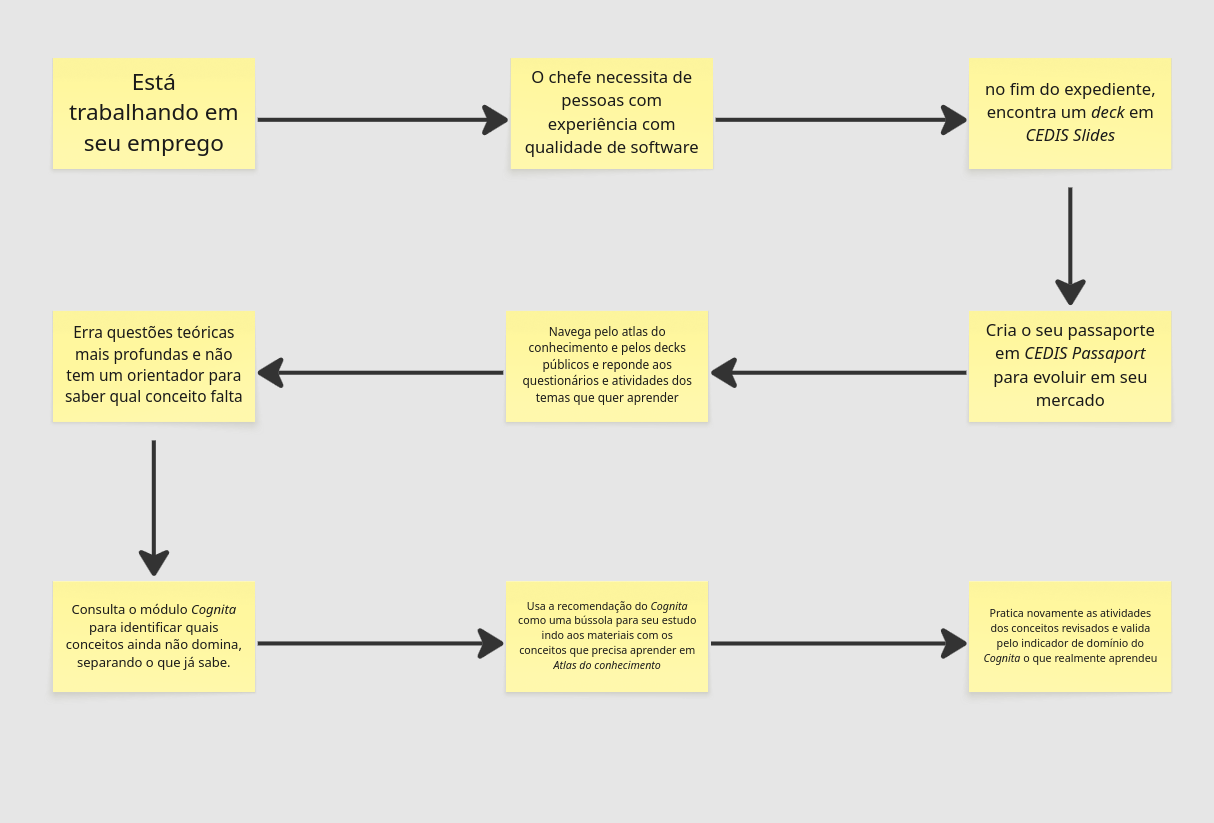
\includegraphics[width=\textwidth]{figuras/persona3Jornada.png}
\legend{Fonte: Elaborado pelos autores.}
\end{figure}

O fluxo detalhado na Figura~\ref{fig:jornada-persona-3} evidencia o papel do Cognita como mecanismo de orientação e validação autônoma em nove passos:

\begin{enumerate}
    \item \textbf{Atuação no mercado de trabalho:} O usuário encontra-se no exercício regular de suas atividades profissionais na área de tecnologia;
    \item \textbf{Gatilho de demanda profissional:} Surge no ambiente de trabalho uma necessidade concreta de qualificação, como a demanda de sua liderança por profissionais com domínio em qualidade de software;
    \item \textbf{Descoberta de conteúdo aberto no ecossistema:} Ao final do expediente, buscando materiais técnicos de referência para estudo independente, o profissional localiza um \textit{deck} público no \textbf{CEDIS Slides} voltado ao tema desejado;
    \item \textbf{Adesão ao passaporte de aprendizagem:} Reconhecendo o valor do ecossistema para sua evolução profissional, cria seu passaporte no \textbf{CEDIS Learning Passport} a fim de manter o registro persistente de sua trajetória de estudos;
    \item \textbf{Exploração autônoma e prática:} Utilizando seu tempo livre semanal, navega pelos mapas conceituais do \textbf{Atlas do Conhecimento} e pelos \textit{decks} públicos, respondendo aos questionários e atividades dos temas que deseja dominar;
    \item \textbf{Barreira na autoavaliação conceitual (Ponto de dor):} Ao deparar-se com questões teóricas mais profundas, comete erros e, por estudar de forma independente sem o suporte de um professor ou orientador acadêmico, não consegue diagnosticar sozinho qual conceito de base está faltando em sua formação prática;
    \item \textbf{Diagnóstico de lacunas no Módulo Cognita (Ponto de contato central):} O estudante consulta o \textbf{Módulo Cognita} para identificar objetivamente quais conceitos fundamentais ainda não domina, distinguindo com nitidez o conhecimento prático já consolidado das lacunas teóricas ocultas;
    \item \textbf{Estudo orientado pelo Cognita:} Utiliza a recomendação do Cognita como um guia de estudos, na ausência de uma grade curricular, dirigindo-se diretamente aos materiais dos conceitos pré-requisitos indicados no \textbf{Atlas do Conhecimento};
    \item \textbf{Consolidação e validação autônoma de domínio:} Após o estudo focado, pratica novamente as atividades vinculadas aos conceitos revisados e valida, por meio da atualização do indicador de domínio no Cognita, que efetivamente assimilou a base teórica necessária para progredir em sua carreira.
\end{enumerate}

\section{Requisitos}
\label{sec:requisitos}

A especificação dos requisitos do módulo Cognita decorreu diretamente dos artefatos produzidos na Seção~\ref{sec:visao-produto}, em especial das jornadas de usuário descritas na Seção~\ref{subsec:jornadas-usuario}, que evidenciaram os pontos de contato nos quais o módulo deve intervir. A partir desse mapeamento, conduziu-se a atividade de \textit{Brainstorming} de Funcionalidades da \textit{Lean Inception} \cite{caroli_lean_2018}, cujo objetivo é traduzir as necessidades e os pontos de dor das personas em funcionalidades candidatas. A atividade foi conduzida de modo a contemplar o fluxo completo das jornadas dos usuários, resultando no conjunto de requisitos funcionais do módulo.

Os requisitos resultantes foram submetidos a \textit{feedbacks} de Sérgio Freitas, responsável pelo Ecossistema CEDIS e cliente do projeto, e, em seguida, à atividade de Revisão Técnica, de Negócio e de UX da \textit{Lean Inception} (Seção~\ref{subsubsec:lean-inception}). Nessa atividade, cada requisito é avaliado quanto a quatro atributos: a dificuldade de aplicabilidade, o esforço de implementação, o valor agregado ao produto e a contribuição para a experiência do usuário. A Figura~\ref{fig:requisitos-priorizacao} apresenta o artefato resultante, no qual cada cartão representa um requisito: a cor indica a dificuldade de aplicabilidade, e as quantidades de símbolos \textit{E}, \$ e $\heartsuit$ indicam, respectivamente, as pontuações de esforço, de valor agregado e de experiência do usuário. Os atributos de cada requisito são detalhados na Tabela~\ref{tab:atributos-requisitos}.

\begin{figure}[H]
\caption{Artefato da atividade de Revisão Técnica, de Negócio e de UX na \textit{Lean Inception}}
\label{fig:requisitos-priorizacao}
\centering
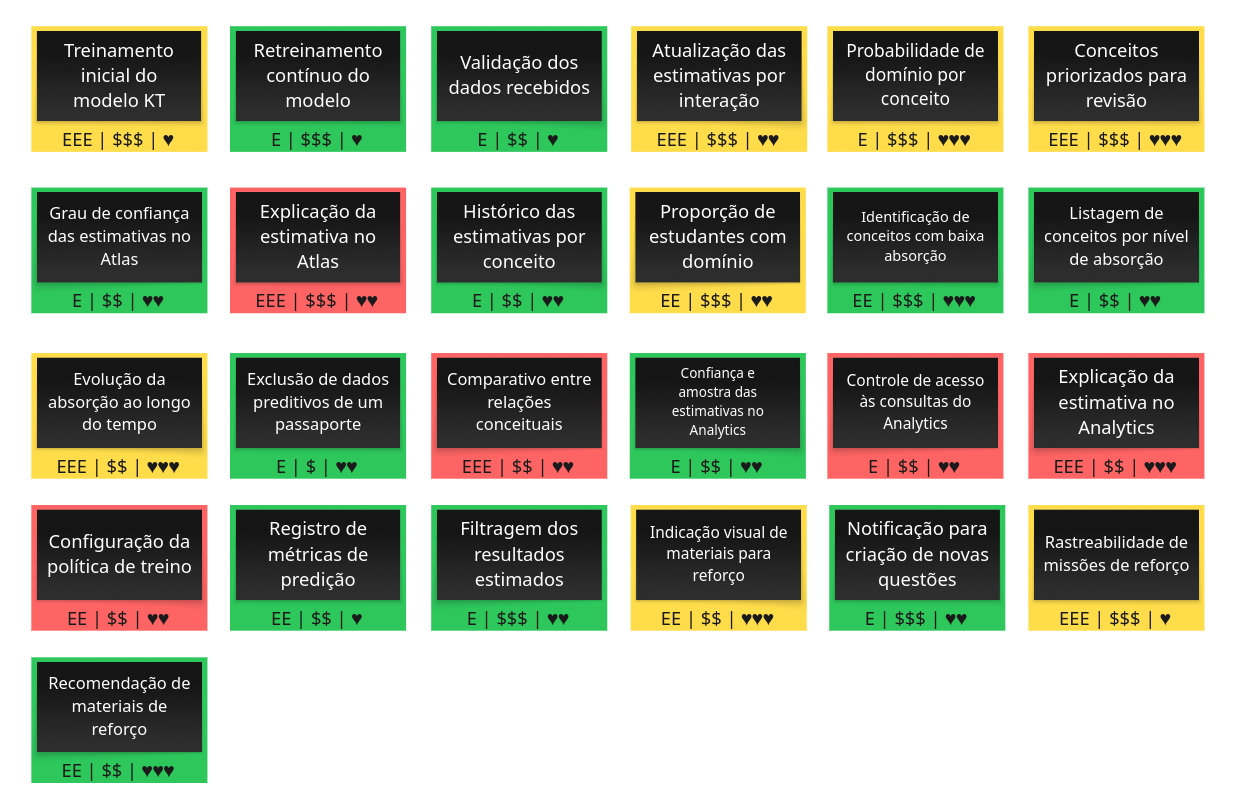
\includegraphics[width=\textwidth]{figuras/requisitos.png}
\legend{Fonte: Elaborado pelos autores.}
\end{figure}

Os atributos avaliados e os significados de seus possíveis valores são os seguintes:

\begin{itemize}
    \item \textbf{Dificuldade de aplicabilidade (cor):} indica o quão difícil é, para os desenvolvedores, aplicar o requisito, considerando o entendimento do requisito e a facilidade de implementá-lo:
    \begin{itemize}
        \item \textit{Fácil} (verde): requisito bem compreendido e de implementação direta;
        \item \textit{Média} (amarelo): requisito com alguma complexidade ou incerteza de implementação;
        \item \textit{Difícil} (vermelho): requisito de implementação complexa ou com alto grau de incerteza.
    \end{itemize}
    \item \textbf{Pontuação de esforço (\textit{E}):} indica o esforço necessário para implementar o requisito:
    \begin{itemize}
        \item 1: Baixo esforço para implementar;
        \item 2: Médio esforço para implementar;
        \item 3: Alto esforço para implementar.
    \end{itemize}
    \item \textbf{Pontuação de valor agregado (\$):} indica o valor que o requisito agrega ao produto:
    \begin{itemize}
        \item 1: Baixo valor agregado ao produto;
        \item 2: Médio valor agregado ao produto;
        \item 3: Alto valor agregado ao produto.
    \end{itemize}
    \item \textbf{Pontuação de experiência do usuário ($\heartsuit$):} indica a contribuição do requisito para a experiência do usuário (\textit{UX}):
    \begin{itemize}
        \item 1: Baixa contribuição para a experiência do usuário;
        \item 2: Média contribuição para a experiência do usuário;
        \item 3: Alta contribuição para a experiência do usuário.
    \end{itemize}
\end{itemize}

A dificuldade de aplicabilidade, o esforço e a contribuição para a experiência do usuário foram definidos em conjunto pelos autores e desenvolvedores do projeto, com base no entendimento de cada requisito, na facilidade de implementá-lo e no seu impacto sobre a interação dos usuários, e posteriormente validados por Sérgio Freitas. Já o valor agregado ao produto foi definido diretamente por Sérgio Freitas, por meio de um formulário submetido com todos os requisitos, no qual as pontuações eram escolhidas com base na descrição de cada requisito. O resultado desse formulário está disponível no Apêndice~\ref{ap:materiais}.

{\small
\begin{longtable}{>{\raggedright\arraybackslash}p{6.0cm}>{\raggedright\arraybackslash}p{2.2cm}>{\centering\arraybackslash}p{1.5cm}>{\centering\arraybackslash}p{2.0cm}>{\centering\arraybackslash}p{1.0cm}}
\caption{Atributos dos requisitos funcionais (dificuldade de aplicabilidade, esforço, valor agregado e UX)}
\label{tab:atributos-requisitos} \\
\hline
\textbf{Requisito} & \textbf{Dificuldade} & \textbf{Esforço} & \textbf{Valor agregado} & \textbf{UX} \\
\hline
\endfirsthead
\caption[]{Atributos dos requisitos funcionais (continuação)} \\
\hline
\textbf{Requisito} & \textbf{Dificuldade} & \textbf{Esforço} & \textbf{Valor agregado} & \textbf{UX} \\
\hline
\endhead
\hline
\multicolumn{5}{r}{\textit{Continua na próxima página}} \\
\endfoot
\hline
\multicolumn{5}{l}{Fonte: Elaborado pelos autores.} \\
\endlastfoot
Treinamento inicial do modelo KT & Média & 3 & 3 & 1 \\
\hline
Retreinamento contínuo do modelo & Fácil & 1 & 3 & 1 \\
\hline
Validação dos dados recebidos & Fácil & 1 & 2 & 1 \\
\hline
Configuração da política de treino & Difícil & 2 & 2 & 2 \\
\hline
Registro de métricas de predição & Fácil & 2 & 2 & 1 \\
\hline
Probabilidade de domínio por conceito & Média & 1 & 3 & 3 \\
\hline
Atualização das estimativas por interação & Média & 3 & 3 & 2 \\
\hline
Conceitos priorizados para revisão & Média & 3 & 3 & 3 \\
\hline
Histórico das estimativas por conceito & Fácil & 1 & 2 & 2 \\
\hline
Evolução da absorção ao longo do tempo & Média & 3 & 2 & 3 \\
\hline
Proporção de estudantes com domínio & Média & 2 & 3 & 2 \\
\hline
Identificação de conceitos com baixa absorção & Fácil & 2 & 3 & 3 \\
\hline
Listagem de conceitos por nível de absorção & Fácil & 1 & 2 & 2 \\
\hline
Comparativo entre relações conceituais & Difícil & 3 & 2 & 2 \\
\hline
Filtragem dos resultados estimados & Fácil & 1 & 3 & 2 \\
\hline
Grau de confiança das estimativas no Atlas & Fácil & 1 & 2 & 2 \\
\hline
Explicação da estimativa no Atlas & Difícil & 3 & 3 & 2 \\
\hline
Confiança e amostra das estimativas no Analytics & Fácil & 1 & 2 & 2 \\
\hline
Explicação da estimativa no Analytics & Difícil & 3 & 2 & 3 \\
\hline
Indicação visual de materiais para reforço & Média & 2 & 2 & 3 \\
\hline
Notificação para criação de novas questões & Fácil & 1 & 3 & 2 \\
\hline
Rastreabilidade de missões de reforço & Média & 3 & 3 & 1 \\
\hline
Recomendação de materiais de reforço & Fácil & 2 & 2 & 3 \\
\hline
Exclusão de dados preditivos de um passaporte & Fácil & 1 & 1 & 2 \\
\hline
Controle de acesso às consultas do Analytics & Difícil & 1 & 2 & 2 \\
\hline
\end{longtable}
}

\subsection{Temas, Épicos e Requisitos Funcionais}
\label{subsec:requisitos-funcionais}

Concluída a Revisão Técnica, de Negócio e de UX, os requisitos foram detalhados pelos próprios desenvolvedores, com base no entendimento do produto consolidado ao longo de toda a \textit{Lean Inception}. O detalhamento seguiu uma estrutura hierárquica de três níveis: os \textbf{temas}, que agrupam as grandes áreas de valor do produto; os \textbf{épicos}, que decompõem cada tema em objetivos funcionais coesos; e as \textbf{histórias de usuário}, que descrevem cada requisito no formato ``O <usuário> deverá <ação>, para que <benefício>''.

Concluído o detalhamento, Sérgio Freitas validou novamente os requisitos, avaliando se contemplavam o que era esperado e se não havia ambiguidade em sua própria interpretação. A versão validada pode ser consultada na Tabela~\ref{tab:temas}, que apresenta o tema do Cognita, na Tabela~\ref{tab:epicos}, que apresenta os épicos associados a esse tema, e na Tabela~\ref{tab:requisitos-funcionais}, que apresenta os requisitos funcionais, cada um associado ao épico ao qual pertence.

% Futuramente: temas definidos na Lean Inception.
\begin{table}[H]
\caption{Temas do Cognita}
\label{tab:temas}
\centering
\begin{tabularx}{\textwidth}{l>{\raggedright\arraybackslash}p{3.2cm}>{\raggedright\arraybackslash}X}
\hline
\textbf{Código} & \textbf{Título} & \textbf{Descrição} \\
\hline
TM01 & Módulo Cognita & Módulo de estimativa do domínio de conceitos incorporado ao Ecossistema CEDIS, que estima o domínio conceitual dos estudantes e entrega diagnósticos acionáveis a eles e aos docentes. \\
\hline
\end{tabularx}
\legend{Fonte: Elaborado pelos autores.}
\end{table}

% Futuramente: épicos definidos na Lean Inception.
{\small
\begin{longtable}{>{\raggedright\arraybackslash}p{1.4cm}>{\raggedright\arraybackslash}p{2.0cm}>{\raggedright\arraybackslash}p{3.4cm}>{\raggedright\arraybackslash}p{7.0cm}}
\caption{Épicos do Cognita}
\label{tab:epicos} \\
\hline
\textbf{Código} & \textbf{Tema associado} & \textbf{Título} & \textbf{História de usuário} \\
\hline
\endfirsthead
\caption[]{Épicos do Cognita (continuação)} \\
\hline
\textbf{Código} & \textbf{Tema associado} & \textbf{Título} & \textbf{História de usuário} \\
\hline
\endhead
\hline
\multicolumn{4}{r}{\textit{Continua na próxima página}} \\
\endfoot
\hline
\multicolumn{4}{l}{Fonte: Elaborado pelos autores.} \\
\endlastfoot
EP01 & TM01 & Gestão do modelo preditivo & O sistema deverá treinar, validar, configurar e monitorar o modelo preditivo de forma contínua, para que as estimativas de domínio sejam geradas a partir de dados consistentes e de um modelo confiável. \\
\hline
EP02 & TM01 & Diagnóstico individual de domínio & O estudante deverá acompanhar, no Atlas, o seu domínio de cada conceito, atualizado a cada interação e com a priorização dos conceitos a revisar, para que direcione os seus estudos de forma eficiente. \\
\hline
EP03 & TM01 & Evolução do domínio ao longo do tempo & O professor deverá observar a evolução da absorção dos conceitos de um curso ao longo do tempo, para que avalie o efeito das ações pedagógicas adotadas. \\
\hline
EP04 & TM01 & Diagnóstico de domínio da turma e do curso & O professor deverá analisar, no Analytics, o domínio dos estudantes por conceito de um curso, para que identifique os conceitos críticos e direcione o planejamento das suas ações. \\
\hline
EP05 & TM01 & Transparência das estimativas & O estudante e o professor deverão visualizar o grau de confiança e os motivos das estimativas de domínio, para que compreendam o diagnóstico e confiem nele ao tomar decisões. \\
\hline
EP06 & TM01 & Reforço da aprendizagem & O estudante e o professor deverão contar com ações de reforço voltadas aos conceitos mal absorvidos, para que as dificuldades de aprendizado sejam superadas. \\
\hline
EP07 & TM01 & Privacidade e controle de acesso & O usuário deverá ter os seus dados preditivos protegidos por regras de acesso e pela possibilidade de exclusão, para que a sua privacidade seja preservada, em conformidade com a LGPD. \\
\hline
\end{longtable}
}

% Futuramente: backlog priorizado da Lean Inception.
{\small
\begin{longtable}{>{\raggedright\arraybackslash}p{1.4cm}>{\raggedright\arraybackslash}p{2.0cm}>{\raggedright\arraybackslash}p{3.4cm}>{\raggedright\arraybackslash}p{7.0cm}}
\caption{Requisitos funcionais do Cognita}
\label{tab:requisitos-funcionais} \\
\hline
\textbf{Código} & \textbf{Épico associado} & \textbf{Requisito} & \textbf{História de usuário} \\
\hline
\endfirsthead
\caption[]{Requisitos funcionais do Cognita (continuação)} \\
\hline
\textbf{Código} & \textbf{Épico associado} & \textbf{Requisito} & \textbf{História de usuário} \\
\hline
\endhead
\hline
\multicolumn{4}{r}{\textit{Continua na próxima página}} \\
\endfoot
\hline
\multicolumn{4}{l}{Fonte: Elaborado pelos autores.} \\
\endlastfoot
RF01 & EP01 & Treinamento inicial do modelo KT & O sistema deverá treinar inicialmente um modelo de \textit{Knowledge Tracing} do tipo \textit{Bayesian Knowledge Tracing} (BKT), com parâmetros estimados por conceito a partir dos dados do ecossistema, para que seja possível estimar o domínio conceitual dos estudantes. \\
\hline
RF02 & EP01 & Retreinamento contínuo do modelo & O sistema deverá retreinar continuamente o modelo preditivo com os novos dados recebidos, para que as estimativas se mantenham precisas. \\
\hline
RF03 & EP01 & Validação dos dados recebidos & O sistema deverá validar os dados recebidos, tratando os dados inconsistentes, para que o treinamento e as estimativas não sejam prejudicados por informações incorretas. \\
\hline
RF04 & EP01 & Configuração da política de treino & O professor deverá definir, no Deck Manager, quais de seus \textit{decks} serão considerados no treinamento do modelo preditivo, para que materiais em construção ou com mapeamento provisório não afetem as estimativas. \\
\hline
RF05 & EP01 & Registro de métricas de predição & O sistema deverá registrar as métricas de predição (AUC, acurácia e RMSE) a cada novo treinamento, para que seja possível monitorar e comparar a qualidade do modelo ao longo do tempo. \\
\hline
RF06 & EP02 & Probabilidade de domínio por conceito & O estudante deverá visualizar, no Atlas, a probabilidade de domínio de cada conceito de um curso, para que compreenda o seu nível de aprendizado em cada conceito. \\
\hline
RF07 & EP02 & Atualização das estimativas por interação & O sistema deverá atualizar as estimativas de predição a cada nova interação do estudante no Atlas, para que o estudante visualize o estado de domínio mais recente. \\
\hline
RF08 & EP02 & Conceitos priorizados para revisão & O estudante deverá visualizar, no Atlas, a lista dos conceitos ainda não dominados de um curso, ordenados por prioridade de revisão, para que saiba quais conceitos revisar primeiro. \\
\hline
RF09 & EP03 & Histórico das estimativas por conceito & O sistema deverá armazenar o histórico da estimativa de domínio de cada conceito ao longo do tempo no Atlas, para que seja possível acompanhar a evolução do aprendizado. \\
\hline
RF10 & EP03 & Evolução da absorção ao longo do tempo & O professor deverá observar, no Analytics, a evolução da absorção dos conceitos de um curso ao longo do tempo, para que avalie o efeito das ações pedagógicas adotadas. \\
\hline
RF11 & EP04 & Proporção de estudantes com domínio & O professor deverá visualizar, no Analytics, a proporção estimada de estudantes que dominam cada conceito de um curso, para que conheça o nível de domínio da turma. \\
\hline
RF12 & EP04 & Identificação de conceitos com baixa absorção & O professor deverá identificar, no Analytics e no Concept Studio, os conceitos de um curso com baixa absorção pelos estudantes, para que possa direcionar ações de reforço. \\
\hline
RF13 & EP04 & Listagem de conceitos por nível de absorção & O professor deverá visualizar, no Analytics, os conceitos de um curso ordenados do menor ao maior nível de absorção, para que identifique rapidamente os conceitos mais críticos. \\
\hline
RF14 & EP04 & Comparativo entre relações conceituais & O professor deverá visualizar comparativos entre as relações conceituais inferidas por um modelo de \textit{Deep Knowledge Tracing} (DKT) e o mapeamento manual feito no Concept Studio, para que possa validar e aprimorar o mapa conceitual do curso. \\
\hline
RF15 & EP04 & Filtragem dos resultados estimados & O professor deverá filtrar os resultados estimados no Analytics, para que concentre a análise nos cursos, conceitos ou grupos de interesse. \\
\hline
RF16 & EP05 & Grau de confiança das estimativas no Atlas & O estudante deverá visualizar, no Atlas, o grau de confiança das estimativas de domínio, para que possa avaliar o quanto confiar nas estimativas apresentadas. \\
\hline
RF17 & EP05 & Explicação da estimativa no Atlas & O estudante deverá visualizar, no Atlas, os motivos que levaram à estimativa de domínio de um conceito, para que compreenda como o diagnóstico foi obtido. \\
\hline
RF18 & EP05 & Confiança e amostra das estimativas no Analytics & O professor deverá visualizar, no Analytics, o grau de confiança e a quantidade de estudantes envolvidos em cada estimativa, para que avalie a confiabilidade dos resultados apresentados. \\
\hline
RF19 & EP05 & Explicação da estimativa no Analytics & O professor deverá visualizar, no Analytics, os motivos que levaram às estimativas de domínio, para que compreenda e confie no diagnóstico apresentado. \\
\hline
RF20 & EP06 & Indicação visual de materiais para reforço & O professor deverá visualizar, no Deck Manager, a indicação visual dos materiais que necessitam de reforço dentro de um conceito, para que possa priorizar a revisão desses materiais. \\
\hline
RF21 & EP06 & Notificação para criação de novas questões & O professor deverá ser notificado para criar novas questões, no Concept Studio + Questionários, para conceitos mal absorvidos, para que os estudantes tenham mais oportunidades de prática nesses conceitos. \\
\hline
RF22 & EP06 & Rastreabilidade de missões de reforço & O professor deverá acompanhar, no Atlas, as missões focadas no estudo de conceitos mal absorvidos, para que avalie a adesão e o efeito dessas missões. \\
\hline
RF23 & EP06 & Recomendação de materiais de reforço & O estudante deverá receber, no Atlas, recomendações de materiais do curso de interesse que reforcem os conceitos mal absorvidos, para que consiga superar as suas dificuldades de aprendizado. \\
\hline
RF24 & EP07 & Exclusão de dados preditivos de um passaporte & O usuário deverá solicitar a exclusão dos dados preditivos associados ao seu passaporte, para que tenha o controle sobre os seus dados pessoais, em conformidade com a LGPD. \\
\hline
RF25 & EP07 & Controle de acesso às consultas do Analytics & O sistema deverá aplicar às consultas do Analytics as regras de acesso compartilhado entre os professores de um curso, para que cada professor acesse apenas os dados dos cursos aos quais tem permissão. \\
\hline
\end{longtable}
}

\subsection{Requisitos Não Funcionais}
\label{subsec:requisitos-nao-funcionais}

Os requisitos não funcionais do Cognita foram organizados segundo o modelo URPS+, uma variação do modelo FURPS+ \cite{pressman_engenharia_2021} que omite a categoria de funcionalidade, já tratada nos requisitos funcionais. O modelo classifica os requisitos de qualidade em quatro categorias, complementadas pelo símbolo ``+'', que agrega as restrições impostas ao sistema:

\begin{itemize}
    \item \textbf{Usabilidade (\textit{Usability}):} requisitos relacionados à facilidade de uso e de aprendizado do módulo pelos usuários;
    \item \textbf{Confiabilidade (\textit{Reliability}):} requisitos relacionados à disponibilidade, à tolerância a falhas e à precisão dos resultados produzidos;
    \item \textbf{Desempenho (\textit{Performance}):} requisitos relacionados ao tempo de resposta, à capacidade de processamento e ao uso de recursos;
    \item \textbf{Suportabilidade (\textit{Supportability}):} requisitos relacionados à manutenção, à testabilidade e à configuração do módulo;
    \item \textbf{Restrições de projeto, de implementação, de interface e físicas (+):} limitações impostas, respectivamente, às decisões de projeto, às tecnologias e aos padrões de implementação, à integração com outros sistemas e ao ambiente físico de execução.
\end{itemize}

Os requisitos não funcionais foram construídos primeiramente por introspecção dos desenvolvedores, com base no entendimento do produto adquirido ao longo do projeto. Em seguida, Sérgio Freitas os validou, avaliando se contemplavam o módulo. Para que fossem verificáveis, cada requisito foi definido com uma métrica objetiva. Como o Cognita é um módulo de software executado na infraestrutura do próprio ecossistema, não foram identificadas restrições físicas nem de interface. A versão validada pode ser consultada na Tabela~\ref{tab:requisitos-nao-funcionais}, que os agrupa por categoria do modelo.

{\small
\begin{longtable}{>{\raggedright\arraybackslash}p{2.0cm}>{\raggedright\arraybackslash}p{11.8cm}}
\caption{Requisitos não funcionais do Cognita}
\label{tab:requisitos-nao-funcionais} \\
\hline
\textbf{Código} & \textbf{Descrição} \\
\hline
\endfirsthead
\caption[]{Requisitos não funcionais do Cognita (continuação)} \\
\hline
\textbf{Código} & \textbf{Descrição} \\
\hline
\endhead
\hline
\multicolumn{2}{r}{\textit{Continua na próxima página}} \\
\endfoot
\hline
\multicolumn{2}{l}{Fonte: Elaborado pelos autores.} \\
\endlastfoot
\multicolumn{2}{l}{\textbf{Usabilidade}} \\
\hline
RNF01 & Um estudante deve conseguir identificar, no Atlas, os conceitos que precisa revisar em até 3 interações (cliques) a partir da tela inicial de um curso. \\
\hline
RNF02 & As telas do Cognita devem obter pontuação mínima de 68 pontos na escala \textit{System Usability Scale} (SUS) \cite{brooke_sus_1996} em avaliação de usabilidade realizada com o cliente do projeto e especialistas. \\
\hline
RNF03 & As telas do Cognita devem ser utilizáveis em dispositivos móveis e computadores, sem rolagem horizontal em larguras de tela a partir de 360 pixels. \\
\hline
\multicolumn{2}{l}{\textbf{Confiabilidade}} \\
\hline
RNF04 & O serviço de consulta às estimativas de domínio deve ter disponibilidade mensal mínima de 99\%. \\
\hline
RNF05 & A cada treinamento, o modelo candidato, avaliado por validação cruzada com divisão dos dados por estudante, só deve substituir o modelo em uso se obtiver AUC superior e RMSE inferior aos do modelo de referência (\textit{baseline}) e se sua AUC não for inferior à do modelo vigente em mais de 0,01. \\
\hline
RNF06 & Em caso de falha no retreinamento, o último modelo válido deve permanecer em operação, sem interrupção do serviço de consulta às estimativas. \\
\hline
RNF07 & 100\% dos registros considerados inconsistentes na validação dos dados devem passar por tratamento antes do treinamento, e apenas aqueles cujo tratamento não tiver êxito devem ser descartados, sendo 100\% dos descartes registrados em \textit{log} com o motivo, para auditoria. \\
\hline
\multicolumn{2}{l}{\textbf{Desempenho}} \\
\hline
RNF08 & A consulta às estimativas de domínio de um estudante deve ser respondida em até 2 segundos para 95\% das requisições, com até 50 usuários simultâneos. \\
\hline
RNF09 & As consultas agregadas do Analytics sobre um curso de até 300 estudantes devem ser respondidas em até 5 segundos para 95\% das requisições. \\
\hline
RNF10 & Após a ingestão de uma nova interação do estudante, a estimativa de domínio correspondente deve ser atualizada em até 60 segundos. \\
\hline
RNF11 & O retreinamento do modelo deve ser concluído em até 6 horas, sem aumentar em mais de 10\% o tempo de resposta das consultas durante sua execução. \\
\hline
\multicolumn{2}{l}{\textbf{Suportabilidade}} \\
\hline
RNF12 & Os componentes de ingestão, validação de dados e inferência devem ter cobertura de testes automatizados de, no mínimo, 80\% das linhas de código. \\
\hline
RNF13 & 100\% dos modelos em operação devem ter versão, parâmetros, período dos dados de treino e métricas de predição registrados, de modo a permitir sua rastreabilidade e reprodução. \\
\hline
\multicolumn{2}{l}{\textbf{Restrições de Projeto}} \\
\hline
RNF14 & O Cognita deve processar dados individuais apenas de passaportes com consentimento ativo (\textit{opt-in}) no Learning Passport, e 100\% das estimativas individuais devem estar associadas a identificadores pseudonimizados, em conformidade com a LGPD. \\
\hline
RNF15 & Indicadores agregados no Analytics devem ser suprimidos quando o grupo analisado tiver menos de 5 estudantes (\textit{k}-anonimato com $k = 5$). \\
\hline
RNF16 & Os dados preditivos associados a um passaporte devem ser excluídos em até 48 horas após a solicitação de exclusão. \\
\hline
\multicolumn{2}{l}{\textbf{Restrições de Implementação}} \\
\hline
RNF17 & 100\% das requisições entre o Cognita e os demais produtos do ecossistema devem ser autenticadas por OAuth2/OIDC, ter as mensagens assinadas com HMAC-SHA256 e trafegar por HTTPS com TLS 1.2 ou superior. \\
\hline
\end{longtable}
}


\subsection{MVP e Incrementos}
\label{subsec:mvp-incrementos}

A definição do MVP decorreu da atividade de Ondas (Sequenciador) da \textit{Lean Inception} \cite{caroli_lean_2018}, na qual os requisitos avaliados na etapa anterior são organizados em ondas incrementais de entrega, considerando seus atributos e suas dependências técnicas. Nessa atividade, o marco do MVP delimita a menor entrega capaz de oferecer o valor central do produto: os requisitos posicionados antes desse marco compõem a primeira entrega do Cognita, enquanto os posicionados após ele constituem os incrementos. As Figuras~\ref{fig:ondas-mvp-1} a~\ref{fig:ondas-mvp-3} apresentam o sequenciador resultante.

\begin{figure}[H]
\caption{Sequenciador do Cognita (ondas 1 a 3)}
\label{fig:ondas-mvp-1}
\centering
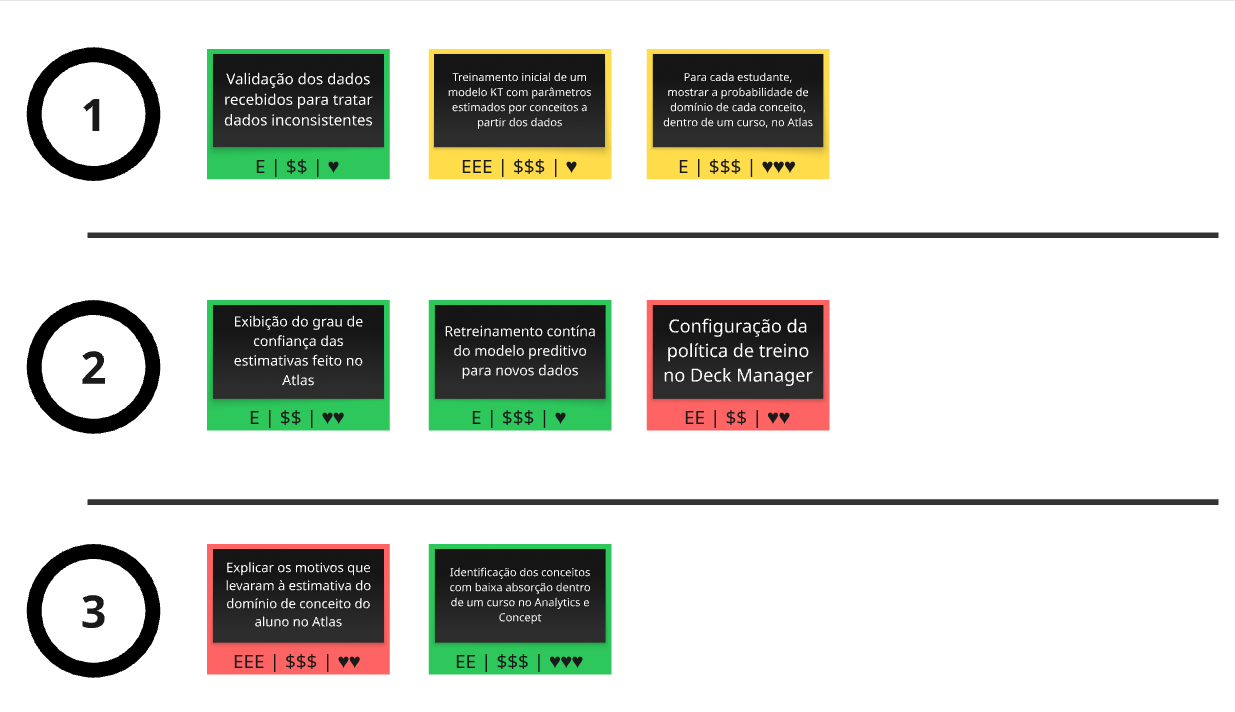
\includegraphics[width=0.9\textwidth]{figuras/sequenciador1.png}
\legend{Fonte: Elaborado pelos autores.}
\end{figure}

\begin{figure}[H]
\caption{Sequenciador do Cognita (ondas 4 a 6)}
\label{fig:ondas-mvp-2}
\centering
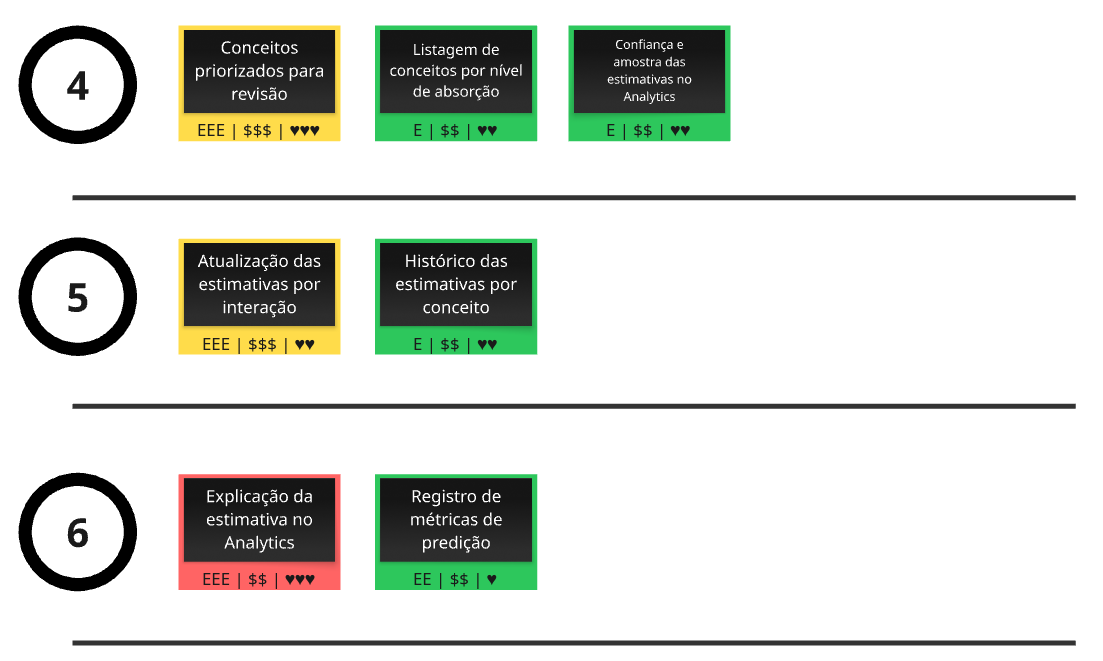
\includegraphics[width=0.9\textwidth]{figuras/sequenciador2.png}
\legend{Fonte: Elaborado pelos autores.}
\end{figure}

\begin{figure}[H]
\caption{Sequenciador do Cognita (ondas 7 a 10 e marcos do MVP e do incremento)}
\label{fig:ondas-mvp-3}
\centering
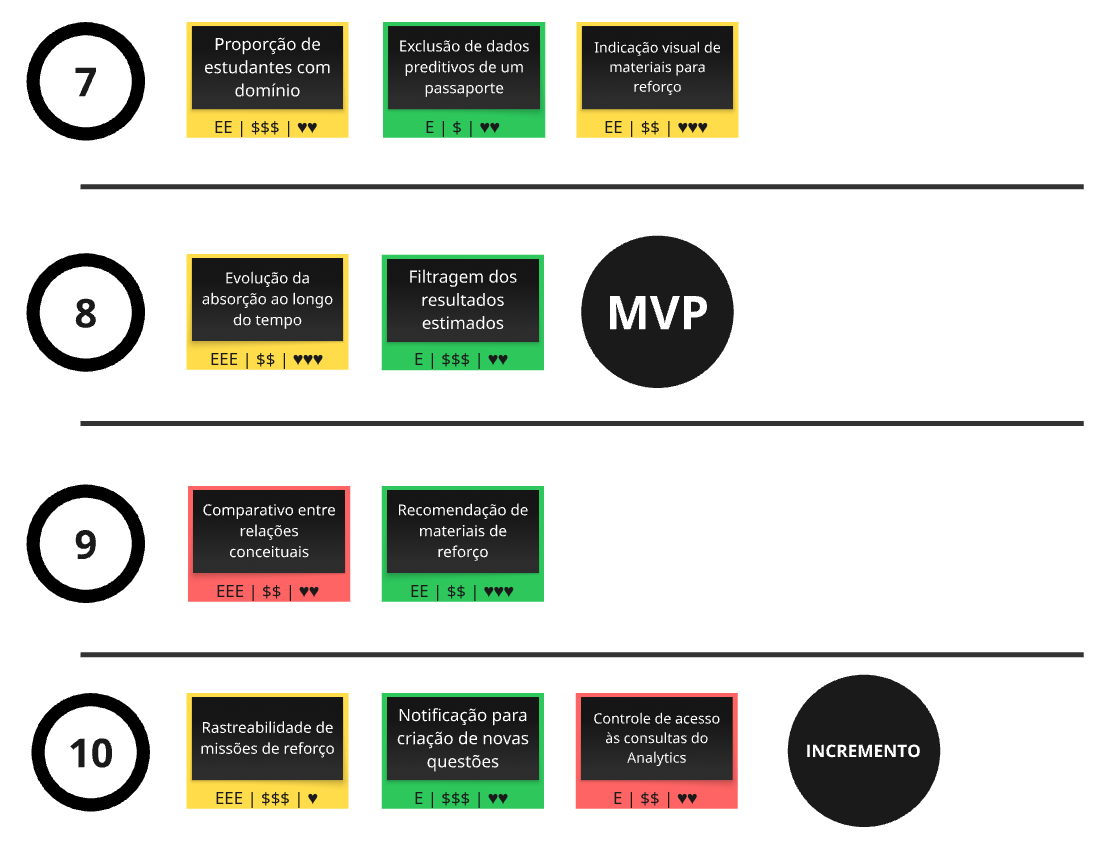
\includegraphics[width=0.9\textwidth]{figuras/sequenciador3.png}
\legend{Fonte: Elaborado pelos autores.}
\end{figure}

A distribuição dos requisitos entre as ondas deve respeitar as seis regras do sequenciador \cite{caroli_lean_2018}, apresentadas a seguir. Nelas, o esforço, o valor agregado e a experiência do usuário de um requisito correspondem às pontuações de 1 a 3 atribuídas a ele na Revisão Técnica, de Negócio e de UX (Tabela~\ref{tab:atributos-requisitos}):

\begin{enumerate}
    \item \textbf{Limite de requisitos:} uma onda pode conter, no máximo, três requisitos;
    \item \textbf{Limite de dificuldade:} uma onda não pode conter mais de um requisito de dificuldade de aplicabilidade difícil (vermelho);
    \item \textbf{Equilíbrio de aplicabilidade:} uma onda com três requisitos não pode ser composta apenas por requisitos amarelos ou vermelhos, devendo conter ao menos um requisito de dificuldade fácil (verde);
    \item \textbf{Limite de esforço:} a soma do esforço dos requisitos de uma onda não pode ultrapassar cinco pontos;
    \item \textbf{Contribuição mínima de valor:} a soma do valor agregado dos requisitos de uma onda deve ser de, no mínimo, quatro pontos, e a soma das pontuações de experiência do usuário também deve ser de, no mínimo, quatro pontos, de modo que cada onda entregue valor de negócio e de UX relevantes;
    \item \textbf{Dependências:} se um requisito depende de outro, o requisito do qual ele depende deve estar em uma onda anterior.
\end{enumerate}

Considerando as regras do sequenciador, os requisitos do MVP foram distribuídos nas oito primeiras ondas da seguinte forma:

\begin{itemize}
    \item \textbf{Primeira onda}
    \begin{itemize}
        \item RF01: Treinamento inicial do modelo KT;
        \item RF03: Validação dos dados recebidos;
        \item RF06: Probabilidade de domínio por conceito.
    \end{itemize}
    \item \textbf{Segunda onda}
    \begin{itemize}
        \item RF02: Retreinamento contínuo do modelo;
        \item RF04: Configuração da política de treino;
        \item RF16: Grau de confiança das estimativas no Atlas.
    \end{itemize}
    \item \textbf{Terceira onda}
    \begin{itemize}
        \item RF12: Identificação de conceitos com baixa absorção;
        \item RF17: Explicação da estimativa no Atlas.
    \end{itemize}
    \item \textbf{Quarta onda}
    \begin{itemize}
        \item RF08: Conceitos priorizados para revisão;
        \item RF13: Listagem de conceitos por nível de absorção;
        \item RF18: Confiança e amostra das estimativas no Analytics.
    \end{itemize}
    \item \textbf{Quinta onda}
    \begin{itemize}
        \item RF07: Atualização das estimativas por interação;
        \item RF09: Histórico das estimativas por conceito.
    \end{itemize}
    \item \textbf{Sexta onda}
    \begin{itemize}
        \item RF05: Registro de métricas de predição;
        \item RF19: Explicação da estimativa no Analytics.
    \end{itemize}
    \item \textbf{Sétima onda}
    \begin{itemize}
        \item RF11: Proporção de estudantes com domínio;
        \item RF20: Indicação visual de materiais para reforço;
        \item RF24: Exclusão de dados preditivos de um passaporte.
    \end{itemize}
    \item \textbf{Oitava onda}
    \begin{itemize}
        \item RF10: Evolução da absorção ao longo do tempo;
        \item RF15: Filtragem dos resultados estimados.
    \end{itemize}
\end{itemize}

Após o marco do MVP, foram posicionados os requisitos classificados como incrementos, os quais não serão entregues no escopo do desenvolvimento deste trabalho:

\begin{itemize}
    \item \textbf{Nona onda}
    \begin{itemize}
        \item RF14: Comparativo entre relações conceituais;
        \item RF23: Recomendação de materiais de reforço.
    \end{itemize}
    \item \textbf{Décima onda}
    \begin{itemize}
        \item RF21: Notificação para criação de novas questões;
        \item RF22: Rastreabilidade de missões de reforço;
        \item RF25: Controle de acesso às consultas do Analytics.
    \end{itemize}
\end{itemize}

Destaca-se que, embora alguns requisitos utilizem resultados de requisitos posicionados em ondas posteriores, essa ordenação não viola a regra de dependências. O RF12 (identificação de conceitos com baixa absorção) e o RF13 (listagem de conceitos por nível de absorção) dependem da proporção de estudantes com domínio em cada conceito, mas o cálculo dessa proporção faz parte da implementação do próprio RF12; o RF11, posicionado na sétima onda, corresponde apenas à exibição dessa proporção ao docente. De forma análoga, o RF02 (retreinamento contínuo) calcula, a cada ciclo, as métricas necessárias ao \textit{Quality Gate}, enquanto o RF05, posicionado na sexta onda, corresponde ao registro histórico dessas métricas para consulta e comparação ao longo do tempo.

\subsection{Canvas MVP}
\label{subsec:mvp-canvas}

Após a validação do Sequenciador pelo cliente, os autores construíram o \textbf{Canvas MVP} (\textit{Minimum Viable Product Canvas}) do módulo Cognita, como etapa de fechamento da \textit{Lean Inception} \cite{caroli_lean_2018}. Esse artefato sintetiza, em sete blocos, a estratégia de validação da primeira entrega do produto, relacionando as personas e as jornadas à proposta de valor, às funcionalidades do MVP, ao cronograma, aos resultados esperados e às métricas de validação. A Figura~\ref{fig:mvp-canvas} apresenta o Canvas MVP do projeto.

\begin{figure}[htb]
\caption{Artefato do Canvas MVP do módulo Cognita na \textit{Lean Inception}}
\label{fig:mvp-canvas}
\centering
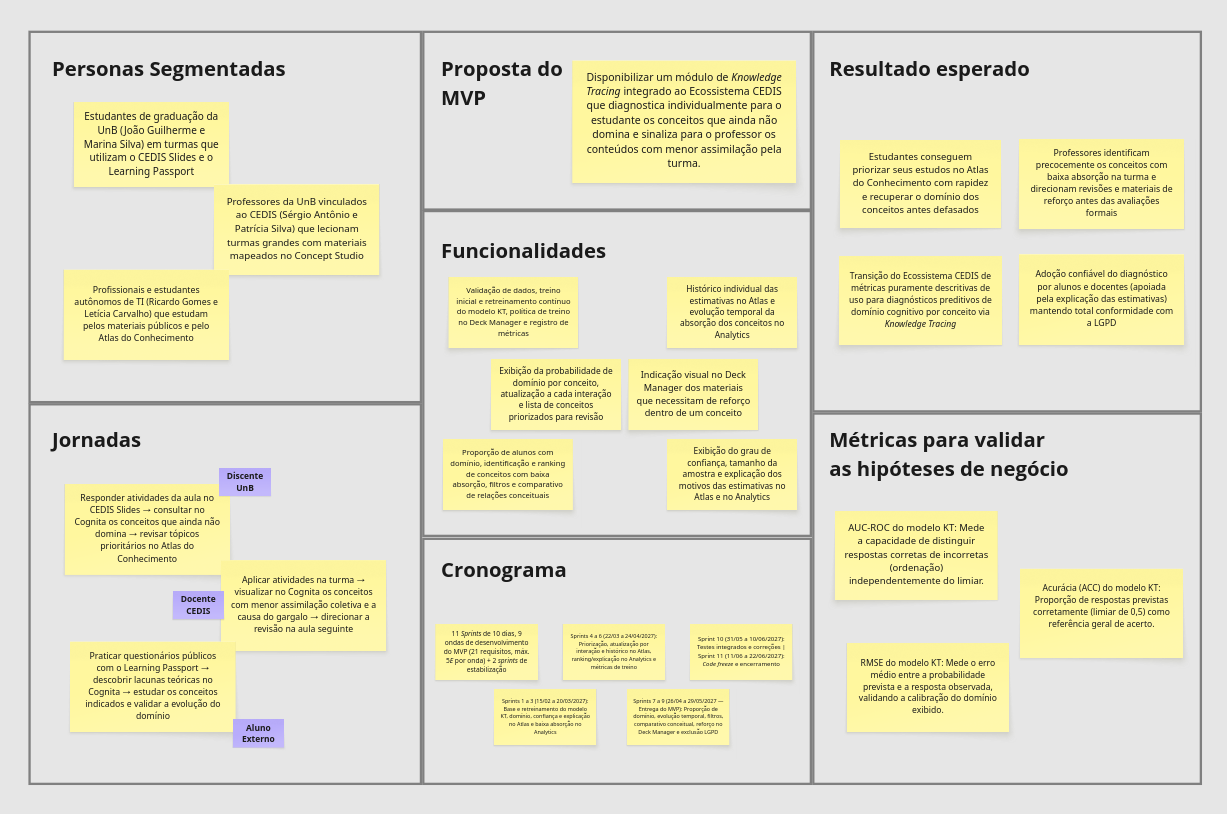
\includegraphics[width=\textwidth]{figuras/CanvasMVP.png}
\legend{Fonte: Elaborado pelos autores.}
\end{figure}

A estruturação dos sete quadrantes da Figura~\ref{fig:mvp-canvas} amarra de forma coesa as decisões de produto e de engenharia adotadas para o Cognita:

\begin{enumerate}
    \item \textbf{Proposta do MVP (Núcleo central de valor):} Define a essência da entrega mínima viável como a disponibilização de um módulo de \textit{Knowledge Tracing} nativamente integrado ao Ecossistema CEDIS, capaz de diagnosticar individualmente para o estudante os conceitos que ele ainda não domina e sinalizar para o professor os conteúdos com menor índice de absorção pela turma.

    \item \textbf{Personas Segmentadas (Público de validação do MVP):} Delimita os três segmentos que utilizarão e validarão o incremento inicial:
    \begin{itemize}
        \item \textit{Segmento Discente Universitário (Foco primário):} Estudantes de graduação da UnB (representados por João Guilherme e Marina Silva) matriculados em turmas que utilizam o CEDIS Slides e o Learning Passport;
        \item \textit{Segmento Docente (Foco primário):} Professores da UnB vinculados ao CEDIS (representados por Marcelo Andrade e Patrícia Silva) que lecionam turmas numerosas com materiais e questões mapeados no Concept Studio;
        \item \textit{Segmento Aprendiz Autônomo (Foco complementar):} Profissionais e estudantes independentes de TI (representados por Ricardo Gomes e Letícia Carvalho) que estudam pelos materiais públicos do ecossistema e pelo Atlas do Conhecimento.
    \end{itemize}

    \item \textbf{Jornadas (Fluxos atendidos pelo MVP):} Sintetiza os três macrofluxos habilitados pelo módulo, identificados pelas etiquetas de perfil no quadro:
    \begin{itemize}
        \item \textit{Discente UnB:} Responder às atividades e aos questionários com o Learning Passport $\rightarrow$ consultar no Cognita os conceitos ainda não dominados $\rightarrow$ revisar os tópicos prioritários no Atlas do Conhecimento;
        \item \textit{Docente CEDIS:} Aplicar atividades na turma $\rightarrow$ visualizar no Cognita os conceitos com menor absorção coletiva e as possíveis origens do gargalo $\rightarrow$ direcionar a revisão pedagógica na aula seguinte;
        \item \textit{Aluno Externo:} Praticar questionários públicos com o Learning Passport $\rightarrow$ descobrir lacunas teóricas no Cognita $\rightarrow$ estudar os conceitos indicados e validar autonomamente a evolução do domínio.
    \end{itemize}

    \item \textbf{Funcionalidades (Escopo funcional enxuto do MVP):} Agrupa os blocos de capacidades que compõem as oito ondas do MVP:
    \begin{itemize}
        \item Validação de dados recebidos, treinamento inicial e retreinamento contínuo do modelo de \textit{Knowledge Tracing} baseado em BKT, configuração da política de treino no Deck Manager e registro de métricas preditivas;
        \item Exibição da probabilidade de domínio por conceito no Atlas do Conhecimento, atualização das estimativas a cada nova interação e listagem de conceitos priorizados para revisão;
        \item Armazenamento do histórico individual das estimativas no Atlas e visualização da evolução temporal da absorção dos conceitos no Learning Analytics;
        \item Estimativa da proporção de alunos com domínio, identificação e ranqueamento de conceitos com baixa absorção e filtragem de resultados;
        \item Transparência e explicabilidade algorítmica por meio da exibição do grau de confiança, tamanho da amostra e explicação dos motivos das estimativas tanto no Atlas quanto no Analytics;
        \item Indicação visual no Deck Manager dos materiais que necessitam de reforço dentro de um conceito e garantia de privacidade mediante exclusão de dados preditivos vinculados ao passaporte em conformidade com a LGPD.
    \end{itemize}

    \item \textbf{Cronograma (Planejamento temporal das entregas):} Estrutura o horizonte de implementação em 11 \textit{Sprints} de aproximadamente 10 dias cada (de 15/02/2027 a 22/06/2027), compreendendo 8 ondas de desenvolvimento para os 20 requisitos do MVP (respeitando o teto de 5 pontos de esforço \textit{E} por onda) e 3 \textit{Sprints} finais de estabilização:
    \begin{itemize}
        \item \textit{Sprints 1 a 3 (15/02 a 20/03/2027):} Base e retreinamento do modelo KT, probabilidade, confiança e explicação de domínio no Atlas e identificação de baixa absorção no Analytics;
        \item \textit{Sprints 4 a 6 (22/03 a 24/04/2027):} Priorização, atualização por interação e histórico no Atlas, ranqueamento e explicação de estimativas no Analytics e registro de métricas de treino;
        \item \textit{Sprints 7 e 8 (26/04 a 18/05/2027, entrega do MVP):} Proporção de domínio, evolução temporal, filtros, indicação de materiais para reforço no Deck Manager e exclusão de dados preditivos (LGPD);
        \item \textit{Sprint 9 (19/05 a 29/05/2027):} Bateria de testes integrados e correções de defeitos;
        \item \textit{Sprints 10 e 11 (31/05 a 22/06/2027):} Congelamento de código (\textit{code freeze}) e encerramento.
    \end{itemize}

    \item \textbf{Resultado Esperado (Hipóteses qualitativas de valor):} Explicita quatro hipóteses de valor: (i) os estudantes priorizam os seus estudos no Atlas do Conhecimento e recuperam o domínio de conceitos defasados; (ii) os professores identificam cedo os conceitos com baixa absorção e direcionam revisões antes das avaliações; (iii) o ecossistema passa de métricas descritivas de uso ao diagnóstico do domínio de conceitos; e (iv) estudantes e docentes adotam o diagnóstico com confiança, apoiados pela explicação das estimativas e pela conformidade com a LGPD.

    \item \textbf{Métricas para Validar as Hipóteses de Negócio (Indicadores quantitativos):} Define as métricas que serão utilizadas para validar as hipóteses do MVP (Seção~\ref{subsec:fase2}):
    \begin{itemize}
        \item \textit{Qualidade preditiva do modelo KT:} AUC-ROC, que mede a capacidade do modelo de distinguir respostas corretas de incorretas independentemente de um limiar de decisão; acurácia (ACC), que avalia a proporção de respostas previstas corretamente; e RMSE, que mede o erro entre a probabilidade prevista e a resposta observada, refletindo a calibração das estimativas. As três métricas são comparadas às de um modelo de referência (\textit{baseline});
        \item \textit{Concordância dos diagnósticos:} correlação entre a absorção dos conceitos estimada pelo Cognita e a absorção percebida pelo docente, que verifica a hipótese (ii);
        \item \textit{Usabilidade:} pontuação na escala SUS, que verifica a hipótese (iv) quanto à facilidade de adoção das telas do módulo.
    \end{itemize}
\end{enumerate}


\section{Arquitetura}
\label{sec:arquitetura}

A arquitetura do módulo Cognita parte do levantamento técnico do Ecossistema CEDIS (Seção~\ref{sec:dados-coletados}) e define como o novo serviço se integra aos componentes, aos bancos de dados e aos contratos de comunicação já em operação \cite{kleppmann_designing_2017, richards_fundamentals_2020}. Esta seção apresenta a arquitetura atual do ecossistema, as APIs que fornecem os dados necessários ao rastreamento de conhecimento e a arquitetura proposta para o módulo.

\subsection{Arquitetura Atual do Ecossistema}
\label{subsec:arquitetura-atual}

A Figura~\ref{fig:arquitetura-atual} representa a arquitetura atual do ecossistema, reconstruída a partir do levantamento técnico do repositório do CEDIS Deck Manager. Trata-se de uma arquitetura distribuída orientada a serviços, na qual cada serviço possui o seu próprio domínio de dados \cite{richards_fundamentals_2020}. O papel de cada componente foi descrito na Tabela~\ref{tab:componentes-cedis}.

\begin{figure}[H]
\caption{Arquitetura atual de serviços e dados do Ecossistema CEDIS}
\label{fig:arquitetura-atual}
\centering
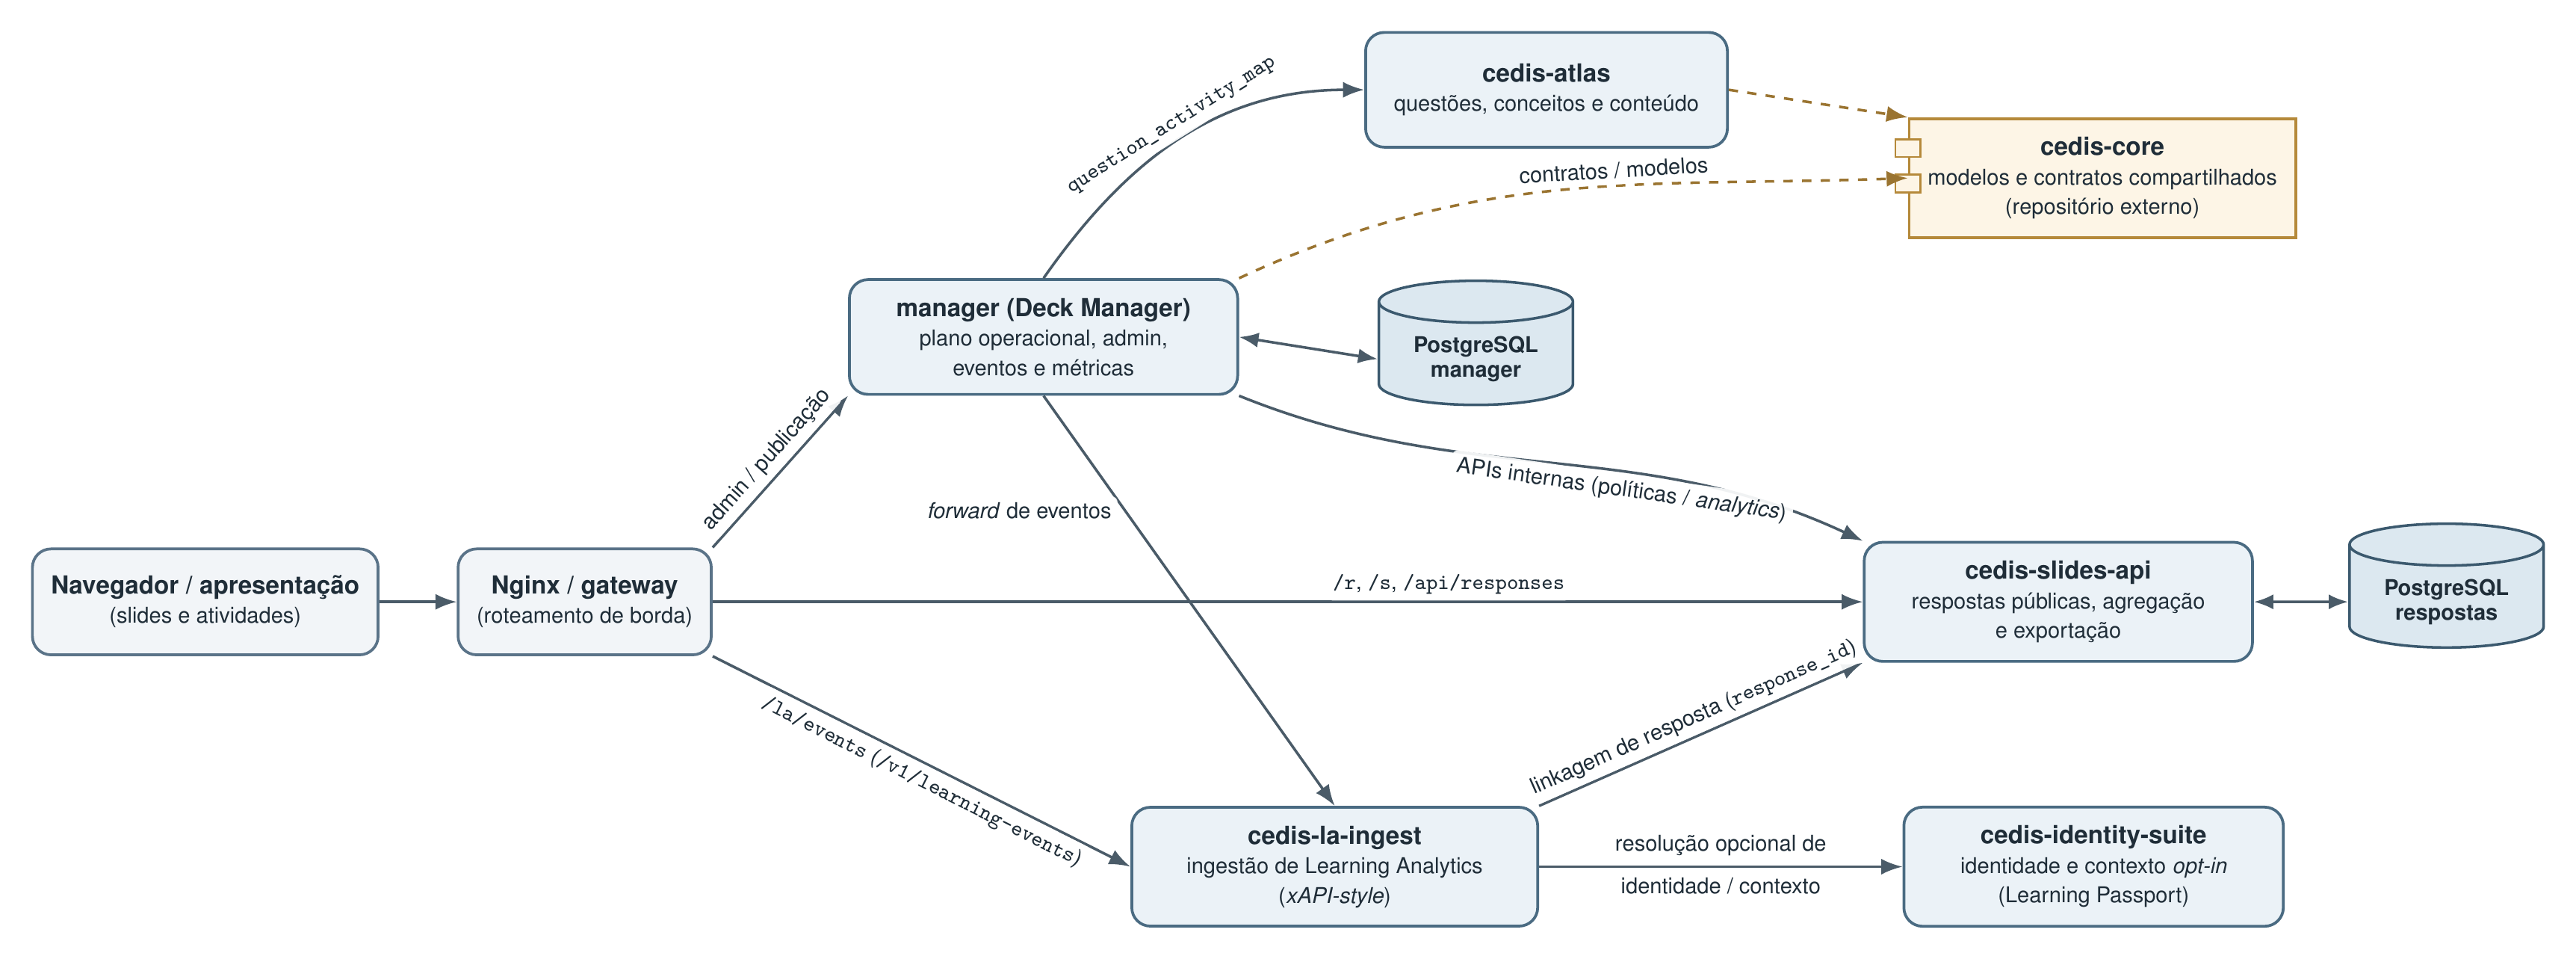
\includegraphics[width=\textwidth]{figuras/arquiteturaAtual.png}
\legend{Fonte: Elaborado pelos autores a partir do levantamento técnico do repositório CEDIS Deck Manager (\textit{commit} \texttt{3bb454a}, 2026).}
\end{figure}

Para o projeto do Cognita, três características dessa arquitetura são determinantes. A primeira é a separação dos fluxos na borda: o navegador comunica-se apenas com o \textit{gateway}, que encaminha os fluxos administrativos ao \textit{manager}, as respostas às atividades ao \textit{cedis-slides-api} e os eventos de aprendizagem ao \textit{cedis-la-ingest}. A segunda é o isolamento da persistência: o \textit{manager} e o \textit{cedis-slides-api} mantêm bancos PostgreSQL próprios, enquanto o \textit{cedis-la-ingest} não possui banco dedicado e apenas articula os vínculos entre respostas, identidade e eventos. A terceira é a existência de ciclos de retenção distintos para a telemetria operacional, para as respostas e para os dados analíticos, o que impede tratar esses registros como equivalentes.

Como cada serviço mantém o seu próprio banco, as relações entre domínios de serviços diferentes não são chaves estrangeiras físicas, mas referências lógicas \cite{kleppmann_designing_2017}. A Figura~\ref{fig:modelo-logico-cross-service} apresenta o modelo lógico do \textit{manager}, reconstruído a partir do código-fonte, com os tipos de dados, a obrigatoriedade dos atributos (\texttt{NN}, \textit{not null}) e as multiplicidades das relações.

\begin{figure}[H]
\caption{Modelo lógico de entidades do \textit{manager} e referências lógicas \textit{cross-service} com os demais serviços do ecossistema}
\label{fig:modelo-logico-cross-service}
\centering
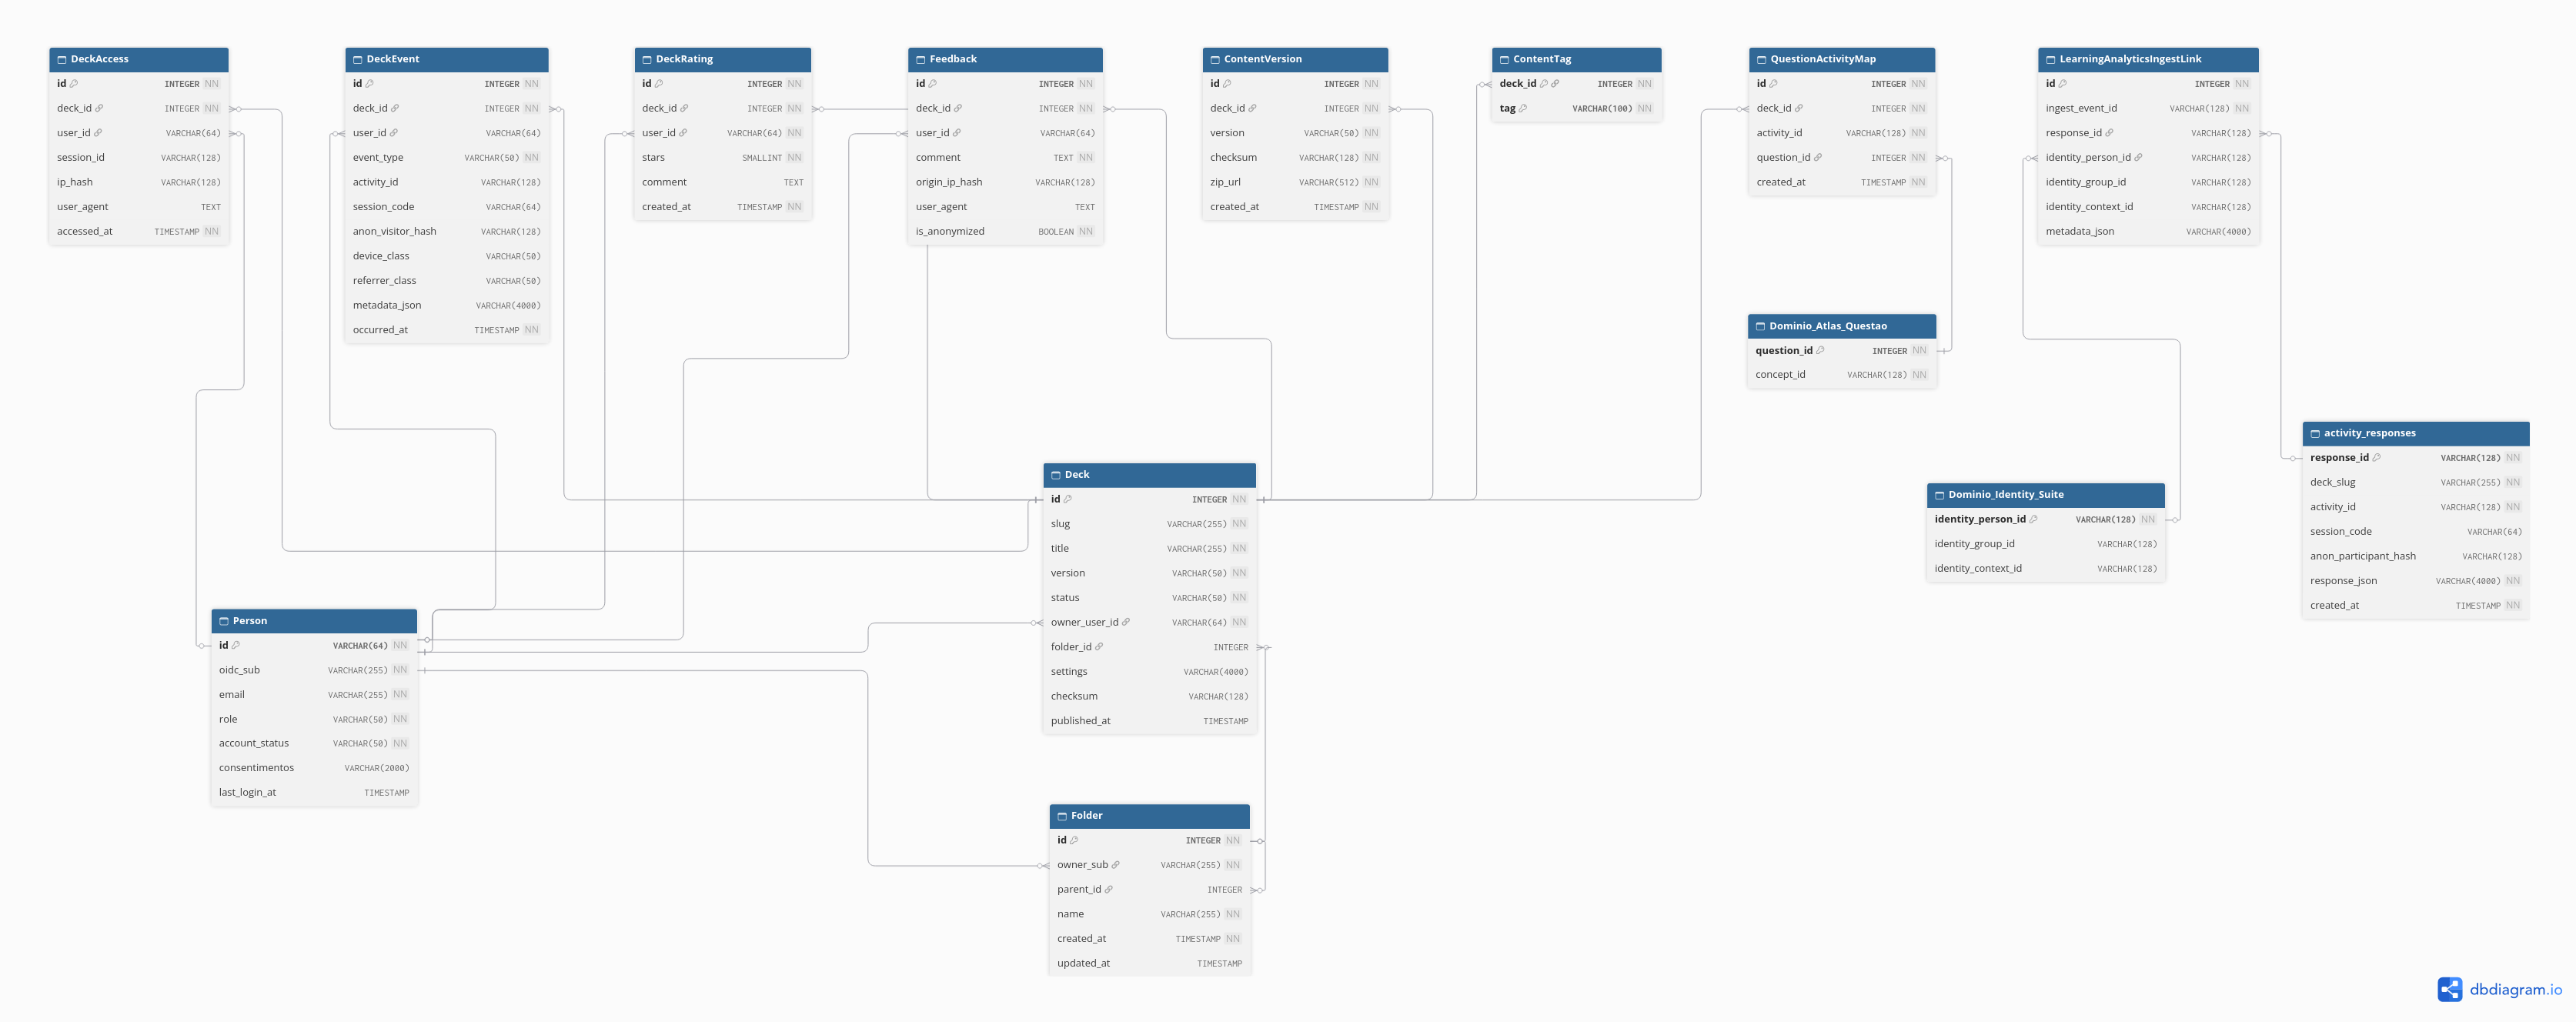
\includegraphics[width=\textwidth]{figuras/ModeloAtual.png}
\legend{Fonte: Elaborado pelos autores a partir do levantamento técnico do repositório CEDIS Deck Manager (\textit{commit} \texttt{3bb454a}, 2026).}
\end{figure}

As entidades internas do \textit{manager}, como \textit{DeckEvent}, \textit{DeckAccess} e \textit{ContentVersion}, relacionam-se fisicamente com \textit{Deck}, \textit{Folder} e com a entidade de usuários (\textit{Person}). Já as entidades \textit{QuestionActivityMap} e \textit{LearningAnalyticsIngestLink}, na porção direita do diagrama, referenciam logicamente três domínios externos: as questões e conceitos do \textit{cedis-atlas} (\textit{Dominio\_Atlas\_Questao}), a identidade consentida do Learning Passport (\textit{Dominio\_Identity\_Suite}) e as respostas do \textit{cedis-slides-api} (\textit{activity\_responses}). Essa estrutura define quatro pontos nos quais o Cognita deve buscar os seus dados:

\begin{itemize}
    \item \textbf{Matriz Q:} o vínculo entre \textit{QuestionActivityMap} e as questões do \textit{cedis-atlas}, que associa cada atividade e questão ao conceito avaliado (\texttt{concept\_id});
    \item \textbf{Desempenho observado:} as respostas registradas em \textit{activity\_responses} e nos questionários do \textit{cedis-atlas}, das quais se extrai a observação $a_t$;
    \item \textbf{Reconciliação e ordenação temporal:} a entidade \textit{LearningAnalyticsIngestLink}, que vincula o evento de aprendizagem à resposta persistida e fornece os carimbos de tempo necessários para ordenar a sequência $X = \{(q_1, a_1), \ldots, (q_t, a_t)\}$;
    \item \textbf{Identidade longitudinal consentida:} o vínculo de \textit{LearningAnalyticsIngestLink} com o Learning Passport (\texttt{identity\_person\_id}), que permite acompanhar o estudante ao longo do tempo apenas quando há consentimento ativo, superando a rotação diária do identificador de telemetria.
\end{itemize}

\subsection{APIs do Ecossistema}
\label{subsec:apis-ecossistema}

Na ausência de chaves estrangeiras entre os bancos dos serviços, a integração do ecossistema depende das suas APIs e dos contratos de dados entre os serviços. Essas integrações utilizam autenticação e autorização via OAuth2 e \textit{OpenID Connect} (OIDC), autorização por \textit{tokens} entre serviços e assinatura de mensagens via HMAC-SHA256. A Figura~\ref{fig:pipeline-coleta-apis} sintetiza os dez estágios pelos quais uma interação passa, desde a captura no navegador até o consumo analítico.

\begin{figure}[H]
\caption{\textit{Pipeline} de coleta, validação, anonimização e reconciliação de dados através das APIs do ecossistema}
\label{fig:pipeline-coleta-apis}
\centering
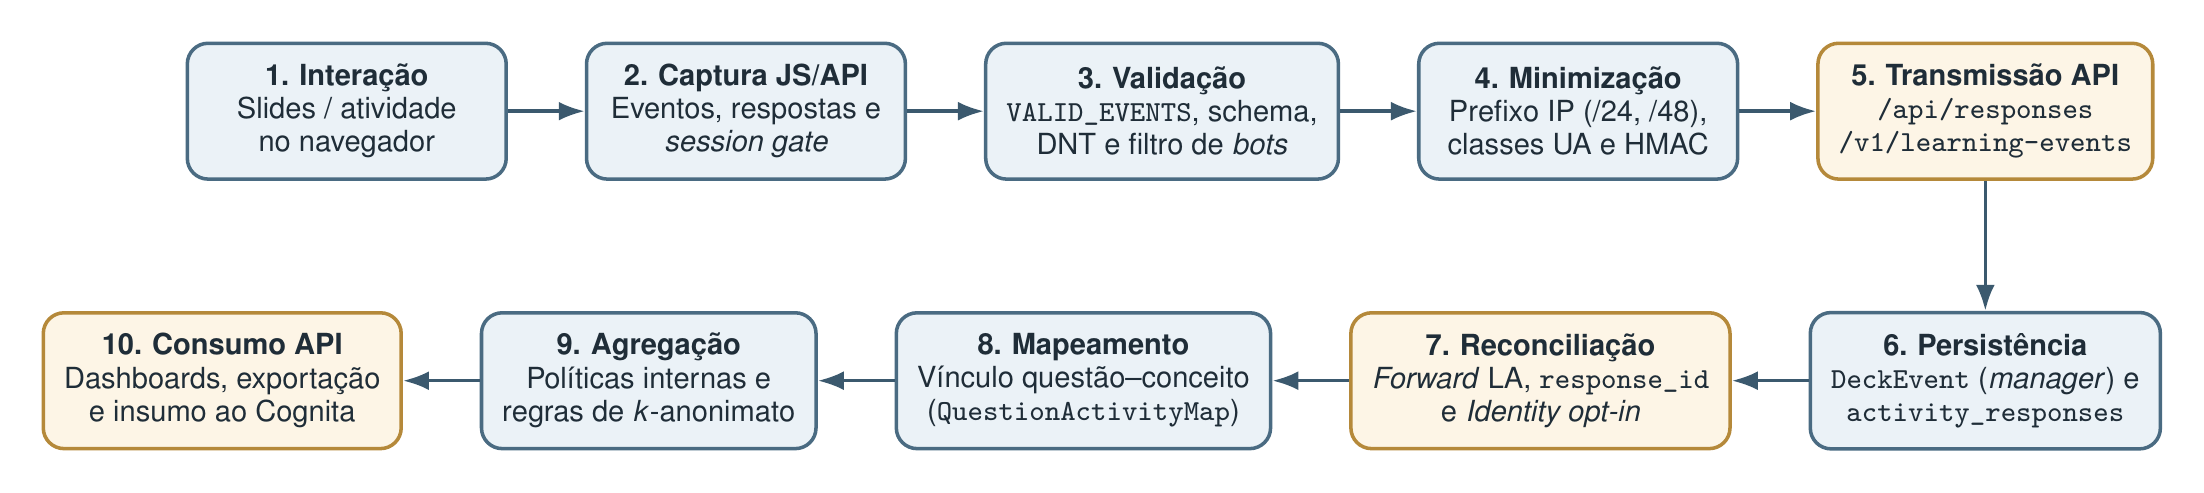
\includegraphics[width=\textwidth]{figuras/pipelineColetaAPIs.png}
\legend{Fonte: Elaborado pelos autores a partir do levantamento técnico do repositório CEDIS Deck Manager (\textit{commit} \texttt{3bb454a}, 2026).}
\end{figure}

Esse \textit{pipeline} é percorrido por três fluxos principais:

\begin{enumerate}
    \item \textbf{Telemetria (\textit{manager}):} os eventos de navegação são validados contra a taxonomia de eventos (estágios 1 a 3), minimizados e pseudonimizados conforme descrito na Seção~\ref{subsec:privacidade} (estágio 4), persistidos em \textit{DeckEvent} (estágio 6) e encaminhados ao \textit{cedis-la-ingest} (estágio 7). Para o Cognita, esse fluxo interessa apenas como fonte auxiliar de carimbos de tempo;
    \item \textbf{Respostas (\textit{cedis-slides-api}):} cada resposta submetida no CEDIS Slides passa pelo controle de acesso da sessão e pela validação do formato (estágios 2 e 3) e é registrada em \textit{activity\_responses}, com o seu identificador (\texttt{response\_id}) e o conteúdo da resposta (\texttt{response\_json}) (estágios 5 e 6). É desse fluxo que provém a evidência de desempenho das atividades em sala de aula;
    \item \textbf{Ingestão de \textit{Learning Analytics} (\textit{cedis-la-ingest}):} os eventos de aprendizagem são recebidos e validados (estágio 5) e vinculados à resposta correspondente e, quando há consentimento, à identidade do estudante no Learning Passport (estágio 7). O vínculo é registrado em \textit{LearningAnalyticsIngestLink} e combinado ao mapeamento questão-conceito de \textit{QuestionActivityMap} (estágio 8).
\end{enumerate}

A Tabela~\ref{tab:apis-ecossistema} sistematiza as APIs e os serviços relevantes para o Cognita, com a responsabilidade de cada um, os dados que fornecem ao módulo e os respectivos \textit{endpoints} e contratos.

{\small
\begin{longtable}{>{\raggedright\arraybackslash}p{2.6cm}>{\raggedright\arraybackslash}p{3.4cm}>{\raggedright\arraybackslash}p{4.3cm}>{\raggedright\arraybackslash}p{3.5cm}}
\caption{APIs e serviços do ecossistema relevantes para o Cognita}
\label{tab:apis-ecossistema} \\
\hline
\textbf{API / Serviço} & \textbf{Responsabilidade} & \textbf{Dados relevantes ao Cognita} & \textbf{Endpoints / contrato} \\
\hline
\endfirsthead
\caption[]{APIs e serviços do ecossistema relevantes para o Cognita (continuação)} \\
\hline
\textbf{API / Serviço} & \textbf{Responsabilidade} & \textbf{Dados relevantes ao Cognita} & \textbf{Endpoints / contrato} \\
\hline
\endhead
\hline
\multicolumn{4}{r}{\textit{Continua na próxima página}} \\
\endfoot
\hline
\multicolumn{4}{l}{Fonte: Elaborado pelos autores a partir do levantamento técnico realizado.} \\
\endlastfoot
\textbf{CEDIS Deck Manager} (\textit{manager}) & Plano operacional, administrativo e analítico; gestão de \textit{decks}, versões, permissões docentes, telemetria (\textit{DeckEvent}), vínculo questão-atividade e reconciliação de LA. & Mapeamento atividade-questão (\textit{QuestionActivityMap}: \textit{deck\_id}, \textit{activity\_id}, \textit{question\_id}); elos de reconciliação (\textit{LearningAnalyticsIngestLink}: \textit{ingest\_event\_id}, \textit{response\_id}, \textit{identity\_*}); metadados e versões de \textit{decks} (\textit{slug}, \textit{version}, \textit{settings}) e permissões de usuários (\textit{User}: \textit{oidc\_sub}, \textit{role}). & Rotas administrativas e de publicação via \textit{gateway}; APIs internas de políticas e \textit{analytics}; \textit{forward} interno de eventos validados (\textit{VALID\_EVENTS}). \\
\hline
\textbf{CEDIS Slides API} (\textit{cedis-slides-api}) & Plano público de coleta de respostas às atividades interativas em tempo real e fornecimento interno de agregações e exportações. & Registros de respostas (\textit{activity\_responses}): identificador da resposta (\textit{response\_id}), \textit{deck} (\textit{deck\_slug}), atividade (\textit{activity\_id}), sessão (\textit{session\_code}), participante pseudonimizado (\textit{anon\_participant\_\allowbreak hash}), conteúdo e correção da resposta (\textit{response\_json}) e instante de registro (\textit{created\_at}). & Rotas públicas de apresentação e submissão (\texttt{/r}, \texttt{/s}, \texttt{POST /api/responses}); endpoints administrativos internos de consulta agregada, exportação e vinculação por \textit{response\_id}. \\
\hline
\textbf{LA Ingest} (\textit{cedis-la-ingest}) & Camada de ingestão de eventos padronizados de \textit{Learning Analytics} (estilo xAPI) e orquestração da vinculação entre eventos, respostas e identidade. & Eventos padronizados de aprendizagem, carimbos de tempo (\textit{occurred\_at}), metadados de duração e interação (\textit{metadata\_json}), e correlação cruzada entre \textit{ingest\_event\_id}, \textit{response\_id} e identificadores de contexto/pessoa. & Rota de borda \texttt{/la/events} (\textit{gateway}) mapeada para \texttt{POST} \texttt{/v1/learning-\allowbreak events} (por \textit{token}); contratos internos de vinculação com \textit{slides-api} e \textit{identity-suite}. \\
\hline
\textbf{Identity Suite / Learning Passport} (\textit{cedis-identity-\allowbreak suite}) & Gestão de identidade persistente pseudonimizada, grupos, contexto acadêmico e controle de consentimento (\textit{opt-in}) e governança de dados pelo estudante (LGPD). & Identificador longitudinal consentido de pessoa (\textit{identity\_person\_id}), grupo/turma (\textit{identity\_group\_id}), contexto (\textit{identity\_context\_id}) e estado ativo de consentimento do titular. & Contrato interno de resolução opcional de identidade/contexto acionado pelo \textit{cedis-la-ingest} sob \textit{opt-in}; autenticação federada e gestão de consentimento. \\
\hline
\textbf{Atlas do Conhecimento e Concept Studio} (\textit{cedis-atlas}) & Estruturação semântica de mapas conceituais, manutenção do banco de conceitos e questões, e interface discente de exploração e prática. & Grafo de conceitos (\textit{Knowledge Concepts}, KC), associação entre questões (\textit{question\_id}) e conceitos (matriz Q), histórico de prática e estrutura de navegação conceitual do estudante. & Integração lógica com o \textit{manager} via \textit{question\_\allowbreak activity\_map} e contratos compartilhados de conteúdo via \textit{cedis-core}. \\
\hline
\textbf{CEDIS Learning Analytics} & Consolidação transversal de indicadores pedagógicos, \textit{dashboards} de turmas e correlações analíticas para apoio à decisão docente. & Indicadores agregados por curso, turma e atividade, séries temporais de engajamento e distribuição de respostas sob políticas de supressão por \textit{k}-anonimato. & Consumo das APIs internas de agregação e telemetria autenticadas via OAuth2/OIDC com controle de acesso baseado em papel (\textit{role}). \\
\hline
\textbf{Pacote Compartilhado} (\textit{cedis-core}) & Biblioteca externa de modelos de domínio e esquemas compartilhados entre os serviços do ecossistema. & Definições estruturais e contratos de validação para entidades de conteúdo, questões e atividades compartilhadas entre o \textit{manager} e o \textit{cedis-atlas}. & Dependência de pacote em repositório externo; fornece esquemas de modelo de domínio versionados por \textit{commit}. \\
\hline
\end{longtable}
}

O levantamento das APIs evidenciou ainda quatro restrições que condicionam o consumo desses dados pelo Cognita:

\begin{enumerate}
    \item \textbf{Assimetria entre evento e resposta:} o evento \textit{activity\_submitted} e a resposta persistida trafegam por rotas distintas, de modo que falhas de rede podem gerar eventos sem resposta ou respostas sem evento. A reconciliação depende, portanto, do identificador \texttt{response\_id} e de mecanismos de idempotência;
    \item \textbf{Heterogeneidade das respostas:} o campo \texttt{response\_json} acomoda formatos diferentes (múltipla escolha, Likert e texto aberto), o que exige filtrar apenas as atividades objetivas antes de extrair $a_t$ (Seção~\ref{subsubsec:oe4});
    \item \textbf{Referências órfãs:} por serem referências lógicas, \texttt{question\_id}, \texttt{response\_id} e \texttt{identity\_person\_id} podem apontar para registros inexistentes, e algumas atividades podem ainda não estar vinculadas a questões;
    \item \textbf{Reprodutibilidade:} como os contratos do \textit{cedis-core} ficam em um repositório separado, cada extração deve registrar a versão desse pacote utilizada, e os carimbos de tempo dos diferentes serviços devem ser normalizados em UTC.
\end{enumerate}

\subsection{Arquitetura Proposta para o Cognita}
\label{subsec:arquitetura-proposta}

A arquitetura do Cognita foi projetada a partir da arquitetura atual, das APIs existentes e dos requisitos da Seção~\ref{sec:requisitos}. Conforme a delimitação de escopo (Seção~\ref{subsubsec:e-nao-e-faz-nao-faz}), o Cognita não possui interface própria: trata-se de um serviço acoplado ao CEDIS Learning Analytics, cujas funcionalidades aparecem nas interfaces das seis aplicações existentes do ecossistema por meio de APIs internas. Para conciliar consultas de baixa latência com o treinamento em lote do modelo, a arquitetura separa o caminho de inferência, executado a cada nova resposta, do caminho de treinamento, executado periodicamente \cite{kleppmann_designing_2017, bass_software_2021}. A Figura~\ref{fig:arquitetura-cognita} apresenta as fontes de dados consumidas (à esquerda), os seis componentes internos e o banco de dados do módulo (ao centro) e as aplicações que exibem os resultados (à direita).

\begin{figure}[H]
\caption{Arquitetura proposta do Cognita integrada ao ecossistema}
\label{fig:arquitetura-cognita}
\centering
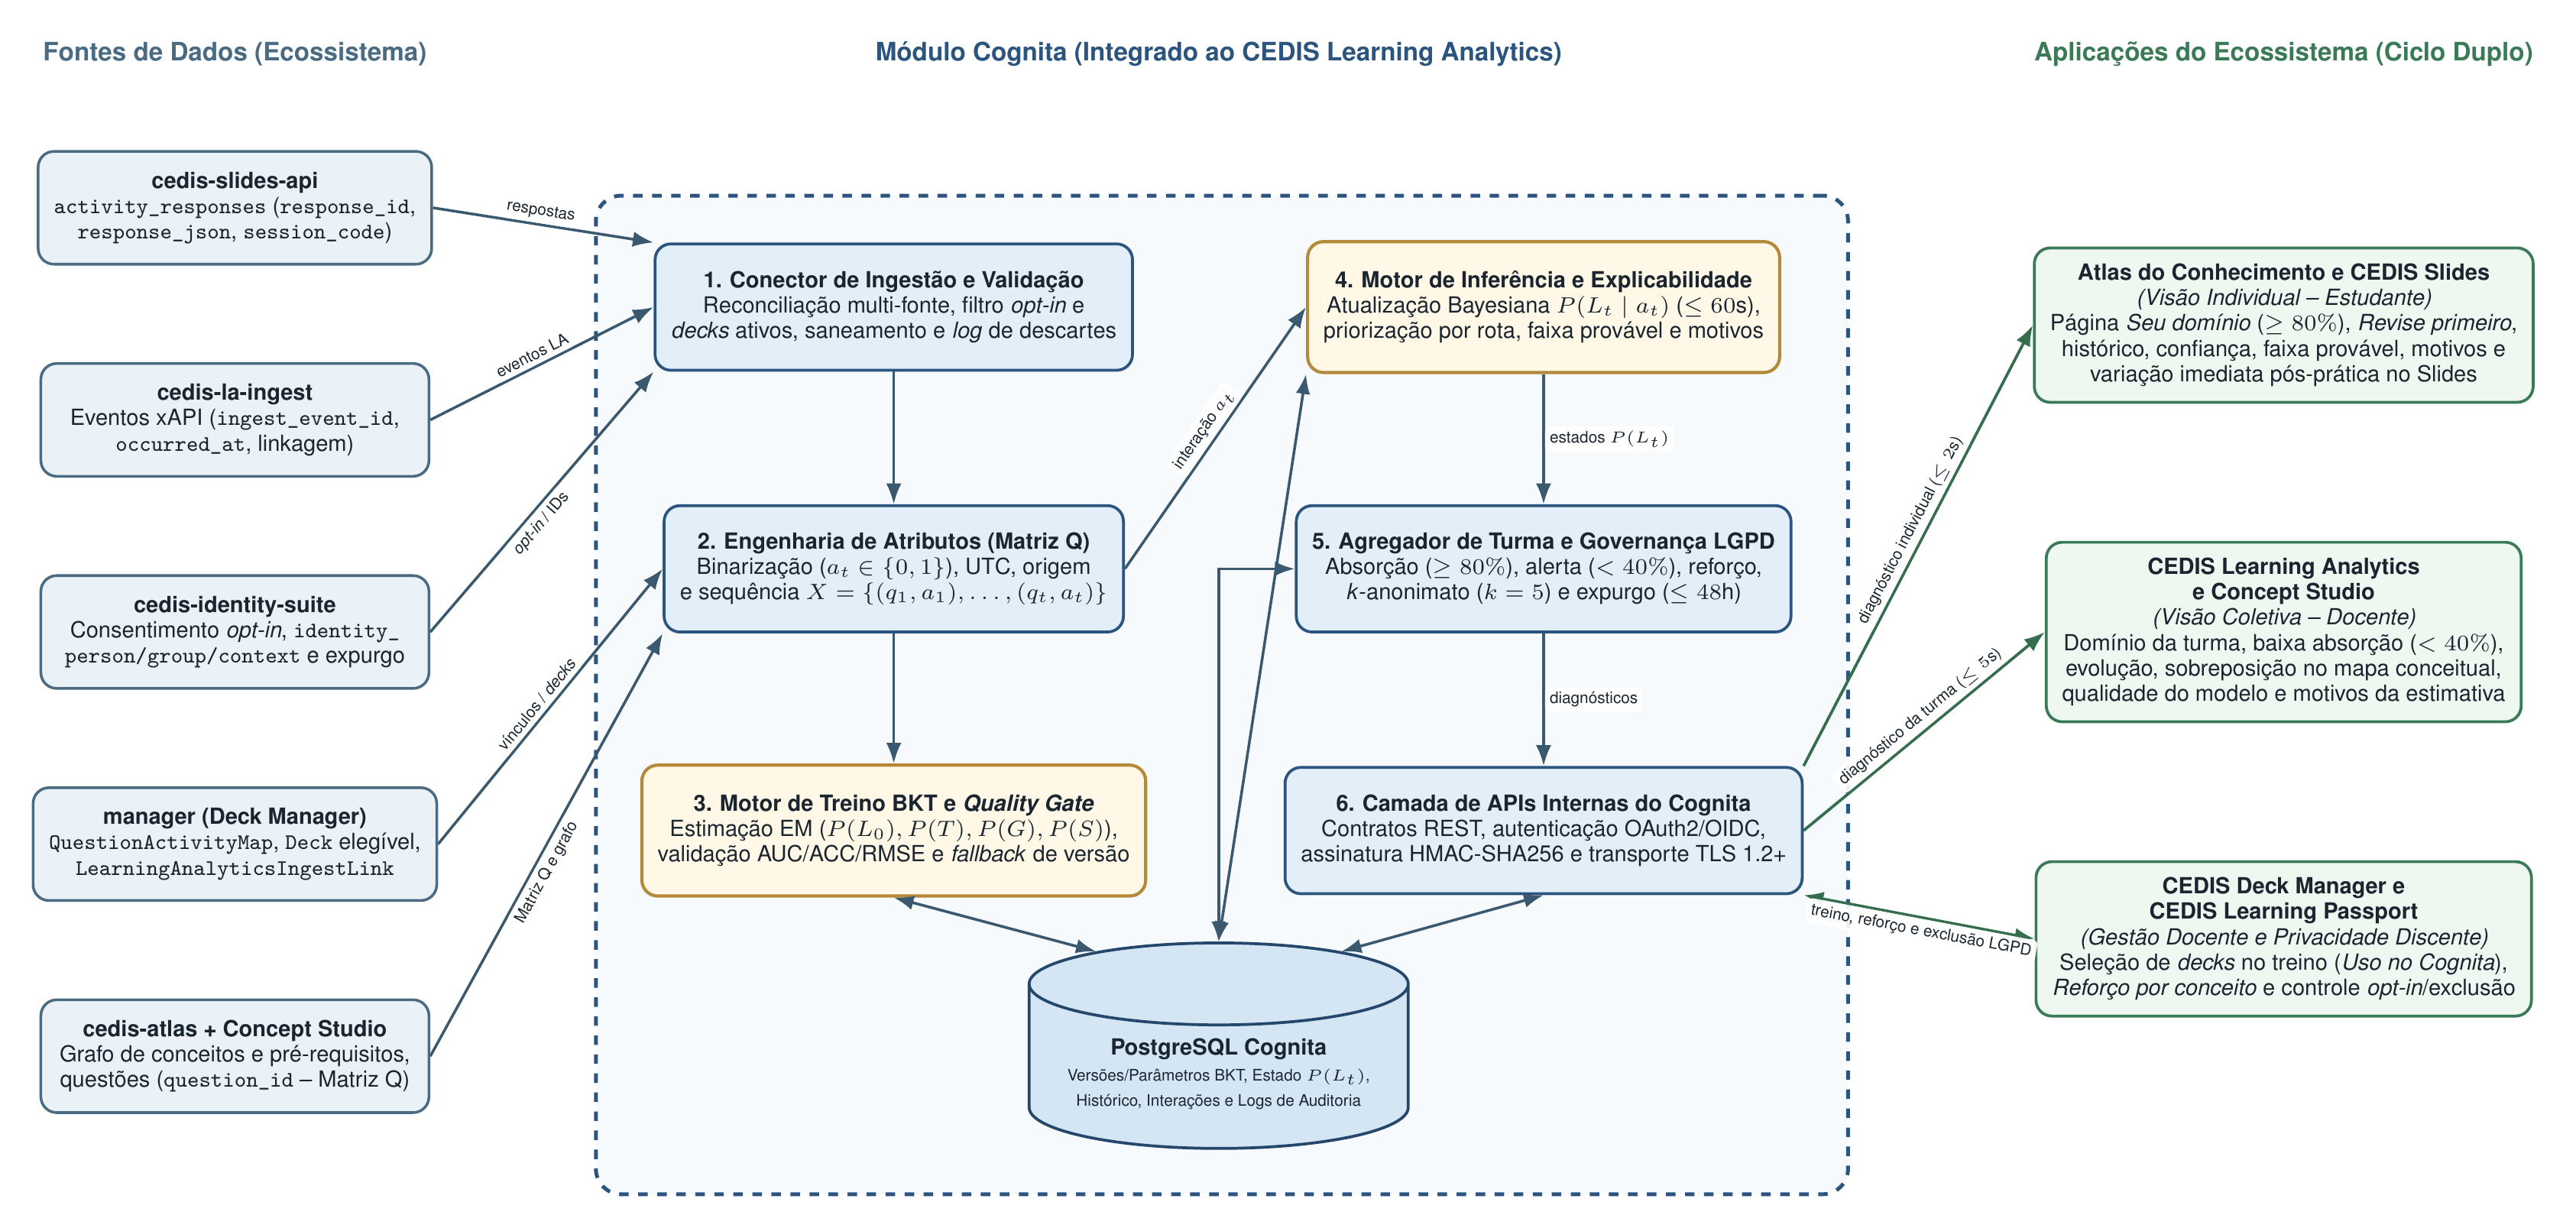
\includegraphics[width=\textwidth]{figuras/arquiteturaCognita.png}
\legend{Fonte: Elaborado pelos autores.}
\end{figure}

Os seis componentes representados na Figura~\ref{fig:arquitetura-cognita} têm as seguintes responsabilidades:

\begin{enumerate}
    \item \textbf{Conector de Ingestão, Validação e Reconciliação:} consome as respostas do CEDIS Slides e do Atlas do Conhecimento, os eventos do \textit{cedis-la-ingest}, o estado de consentimento do Learning Passport, os vínculos e a seleção de \textit{decks} do \textit{manager} e a estrutura de conceitos do \textit{cedis-atlas}. Aplica os critérios de inclusão descritos na Seção~\ref{subsubsec:oe4}, entre eles o consentimento ativo (RNF14) e a habilitação do \textit{deck} pelo docente (RF04), trata as inconsistências recuperáveis, como envios duplicados, e registra os descartes com o respectivo motivo em uma tabela de auditoria (RF03 e RNF07);
    \item \textbf{Engenharia de Atributos e Sequenciamento:} constrói a Matriz Q a partir dos vínculos entre questões e conceitos, importa as relações de pré-requisito do Concept Studio, extrai a observação $a_t$ da primeira tentativa de cada resposta, registra a sua origem (atividade em sala de aula ou questionário individual) e ordena as respostas de cada estudante por conceito, produzindo as sequências consumidas pelo BKT;
    \item \textbf{Motor de Treinamento BKT e \textit{Quality Gate}:} estima os parâmetros do BKT por conceito, com chute e descuido distintos por origem e parâmetros globais para os conceitos com poucas respostas (Seção~\ref{subsubsec:oe4}). O treinamento é disparado por agendamento ou por volume de novas respostas, conforme a política de treino (RF02 e RF04), e é executado em segundo plano, com duração máxima de 6 horas (RNF11). Cada versão candidata é avaliada por validação cruzada agrupada por estudante e só é promovida se superar o modelo de referência e não reduzir a AUC do modelo vigente em mais de 0,01 (RNF05). Caso contrário, a versão anterior permanece em operação (RNF06);
    \item \textbf{Motor de Inferência, Priorização e Explicabilidade:} a cada nova resposta válida, atualiza a probabilidade de domínio do estudante no conceito correspondente por meio das Equações~\ref{eq:bkt-correta} a~\ref{eq:bkt-transicao}, em até 60 segundos (RNF10), e registra a variação na série histórica. Com base nessa probabilidade e nos limiares da Tabela~\ref{tab:limiares}, classifica o conceito como dominado, em progresso, a revisar ou sem evidências, calcula o grau de confiança da estimativa e gera a lista \textit{Revise primeiro}, que prioriza os conceitos de menor domínio que servem de pré-requisito para os próximos destinos da rota do estudante. Também estrutura os motivos da estimativa em linguagem acessível, como o total de acertos e erros e a origem das respostas;
    \item \textbf{Agregador de Turma e Governança LGPD:} consolida as estimativas individuais em indicadores por curso, turma, período e conceito (RF11 a RF15), como a proporção de estudantes com domínio, o ranqueamento dos conceitos por nível de absorção e a evolução semanal dessa absorção. Calcula também a confiança e a amostra das estimativas coletivas (RF18), as explicações para o docente (RF19) e a indicação dos materiais que precisam de reforço (RF20), segundo os limiares da Tabela~\ref{tab:limiares}. No plano da privacidade, suprime os indicadores de grupos com menos de cinco estudantes (RNF15) e executa a exclusão dos dados preditivos de um passaporte em até 48 horas após a solicitação (RF24 e RNF16), sem apagar os dados do estudante nos demais produtos do ecossistema;
    \item \textbf{Camada de APIs Internas:} expõe os resultados às aplicações do ecossistema por meio de \textit{endpoints} REST internos, protegidos por OAuth2/OIDC, assinatura HMAC-SHA256 e transporte HTTPS (RNF17), e atende às metas de disponibilidade e de tempo de resposta definidas nos RNF04, RNF08 e RNF09. Os estados preditivos, as versões do modelo, as séries históricas e os registros de auditoria são armazenados em um banco PostgreSQL próprio, isolado dos bancos dos demais serviços (Seção~\ref{sec:modelagem-dados}).
\end{enumerate}


\section{Modelagem de Dados}
\label{sec:modelagem-dados}

A modelagem de dados do Cognita compreende duas partes: as entidades e os atributos já existentes no Ecossistema CEDIS que servem de entrada para o módulo e o modelo lógico próprio do Cognita, que armazena a política de treino, as versões e os parâmetros do modelo, as interações reconciliadas, as estimativas de domínio e os registros de auditoria.

\subsection{Entidades e Atributos Utilizados}
\label{subsec:entidades-utilizadas}

A Tabela~\ref{tab:entidades-cognita} seleciona, a partir do modelo de dados e dos contratos das APIs do ecossistema (detalhados na Seção~\ref{sec:dados-coletados} e na Seção~\ref{subsec:apis-ecossistema}), as entidades consumidas como entrada pelo módulo Cognita, especificando o serviço de origem, os nomes reais dos atributos utilizados e a finalidade de cada conjunto de dados dentro do módulo.

{\small
\begin{longtable}{>{\raggedright\arraybackslash}p{3.0cm}>{\raggedright\arraybackslash}p{2.4cm}>{\raggedright\arraybackslash}p{3.8cm}>{\raggedright\arraybackslash}p{4.6cm}}
\caption{Entidades do ecossistema utilizadas como entrada do Cognita}
\label{tab:entidades-cognita} \\
\hline
\textbf{Entidade} & \textbf{Origem} & \textbf{Atributos utilizados} & \textbf{Finalidade no Cognita} \\
\hline
\endfirsthead
\caption[]{Entidades do ecossistema utilizadas como entrada do Cognita (continuação)} \\
\hline
\textbf{Entidade} & \textbf{Origem} & \textbf{Atributos utilizados} & \textbf{Finalidade no Cognita} \\
\hline
\endhead
\hline
\multicolumn{4}{r}{\textit{Continua na próxima página}} \\
\endfoot
\hline
\multicolumn{4}{l}{Fonte: Elaborado pelos autores a partir do levantamento técnico realizado.} \\
\endlastfoot
\textit{activity\_\allowbreak responses} & \textit{cedis-slides-api} & \textit{response\_id}, \textit{deck\_slug}, \textit{activity\_id}, \textit{session\_code}, \textit{anon\_participant\_\allowbreak hash}, \textit{response\_json}, \textit{created\_at} & Fonte primária da evidência observável de desempenho ($a_t \in \{0, 1\}$ extraído de \textit{response\_json}), do instante de submissão e da taxa de erro por atividade para identificação de materiais que precisam de reforço. \\
\hline
\textit{LearningAnalytics\allowbreak IngestLink} & \textit{manager} / \textit{cedis-la-ingest} & \textit{id}, \textit{ingest\_event\_id}, \textit{response\_id}, \textit{identity\_person\_id}, \textit{identity\_group\_id}, \textit{identity\_context\_id}, \textit{metadata\_json} & Elo central de reconciliação \textit{cross-service} que vincula o evento de aprendizagem e a resposta persistida ao pseudônimo longitudinal do passaporte do estudante e ao contexto de curso e turma. \\
\hline
\textit{QuestionActivity\allowbreak Map} & \textit{manager} & \textit{id}, \textit{deck\_id}, \textit{activity\_id}, \textit{question\_id}, \textit{created\_at} & Mapeia cada atividade interativa de um \textit{deck} à respectiva questão avaliativa (\textit{question\_id}), permitindo verificar se o \textit{deck} possui mapeamento completo ou parcial para o treino e associar erros aos materiais no Deck Manager. \\
\hline
\textit{DeckEvent} & \textit{manager} & \textit{id}, \textit{deck\_id}, \textit{event\_type}, \textit{activity\_id}, \textit{session\_code}, \textit{occurred\_at}, \textit{metadata\_json} & Fornece o carimbo temporal da interação (\textit{occurred\_at} para \textit{activity\_started} e \textit{activity\_submitted}), auxiliando na deduplicação de envios repetidos e na reordenação cronológica da sequência $X$. \\
\hline
\textit{Deck}, \textit{Folder} e \textit{ContentVersion} & \textit{manager} & \textit{id}, \textit{folder\_id}, \textit{slug}, \textit{title}, \textit{version}, \textit{status}, \textit{owner\_user\_id}, \textit{settings}, \textit{checksum} & Contextualiza a pasta e os \textit{decks} do curso, armazena nas configurações se o \textit{deck} está habilitado para uso no treinamento do Cognita e identifica os materiais que demandam reforço por conceito. \\
\hline
\textit{User} (\textit{Person}) & \textit{manager} & \textit{id}, \textit{oidc\_sub}, \textit{role}, \textit{account\_status} & Autenticação e controle de acesso de docentes e administradores às visões do curso no Learning Analytics, no Concept Studio e à seleção de \textit{decks} de treino no Deck Manager. \\
\hline
\textit{Questões, Conceitos e Relações} (\textit{Dominio\_\allowbreak Atlas\_Questao}) & \textit{cedis-atlas} / Concept Studio / \textit{cedis-core} & \textit{question\_id}, \textit{concept\_id}, relações entre conceitos (pré-requisito, hierarquia, relacionado), destino da rota e gabarito & Define os conceitos (\textit{Knowledge Concepts}, KC), a Matriz Q questão-conceito, as práticas/expedições do Atlas e as relações de pré-requisito usadas na priorização de revisão (\textit{Revise primeiro}) e na explicação de baixa absorção. \\
\hline
\textit{Passaporte e Consentimento} (\textit{Dominio\_\allowbreak Identity\_Suite}) & \textit{cedis-identity-\allowbreak suite} (Learning Passport) & \textit{identity\_person\_id}, \textit{identity\_group\_id}, \textit{identity\_context\_id}, chave de autorização do Cognita (\textit{opt-in}) e evento de exclusão & Garante que o Cognita processe e exiba estimativas individuais apenas para passaportes com autorização ativa e aciona a exclusão exclusiva dos dados preditivos em até 48 horas. \\
\hline
\end{longtable}
}

\subsection{Modelo Lógico de Dados do Módulo Cognita}
\label{subsec:der-cognita}

O modelo lógico relacional do Cognita, apresentado na Figura~\ref{fig:der-cognita}, cobre todo o ciclo de operação do módulo: a política de treino, as versões e os parâmetros do BKT, a auditoria da validação de dados, as estimativas de domínio e o seu histórico, as explicações e a exclusão de dados exigida pela LGPD. A figura indica os tipos de dados, a obrigatoriedade (\texttt{NN}, \textit{not null}) e a unicidade dos atributos, as chaves primárias e estrangeiras e as cardinalidades, em notação \textit{Crow's Foot}.

\begin{figure}[H]
\caption{Modelo lógico de dados do módulo Cognita}
\label{fig:der-cognita}
\centering
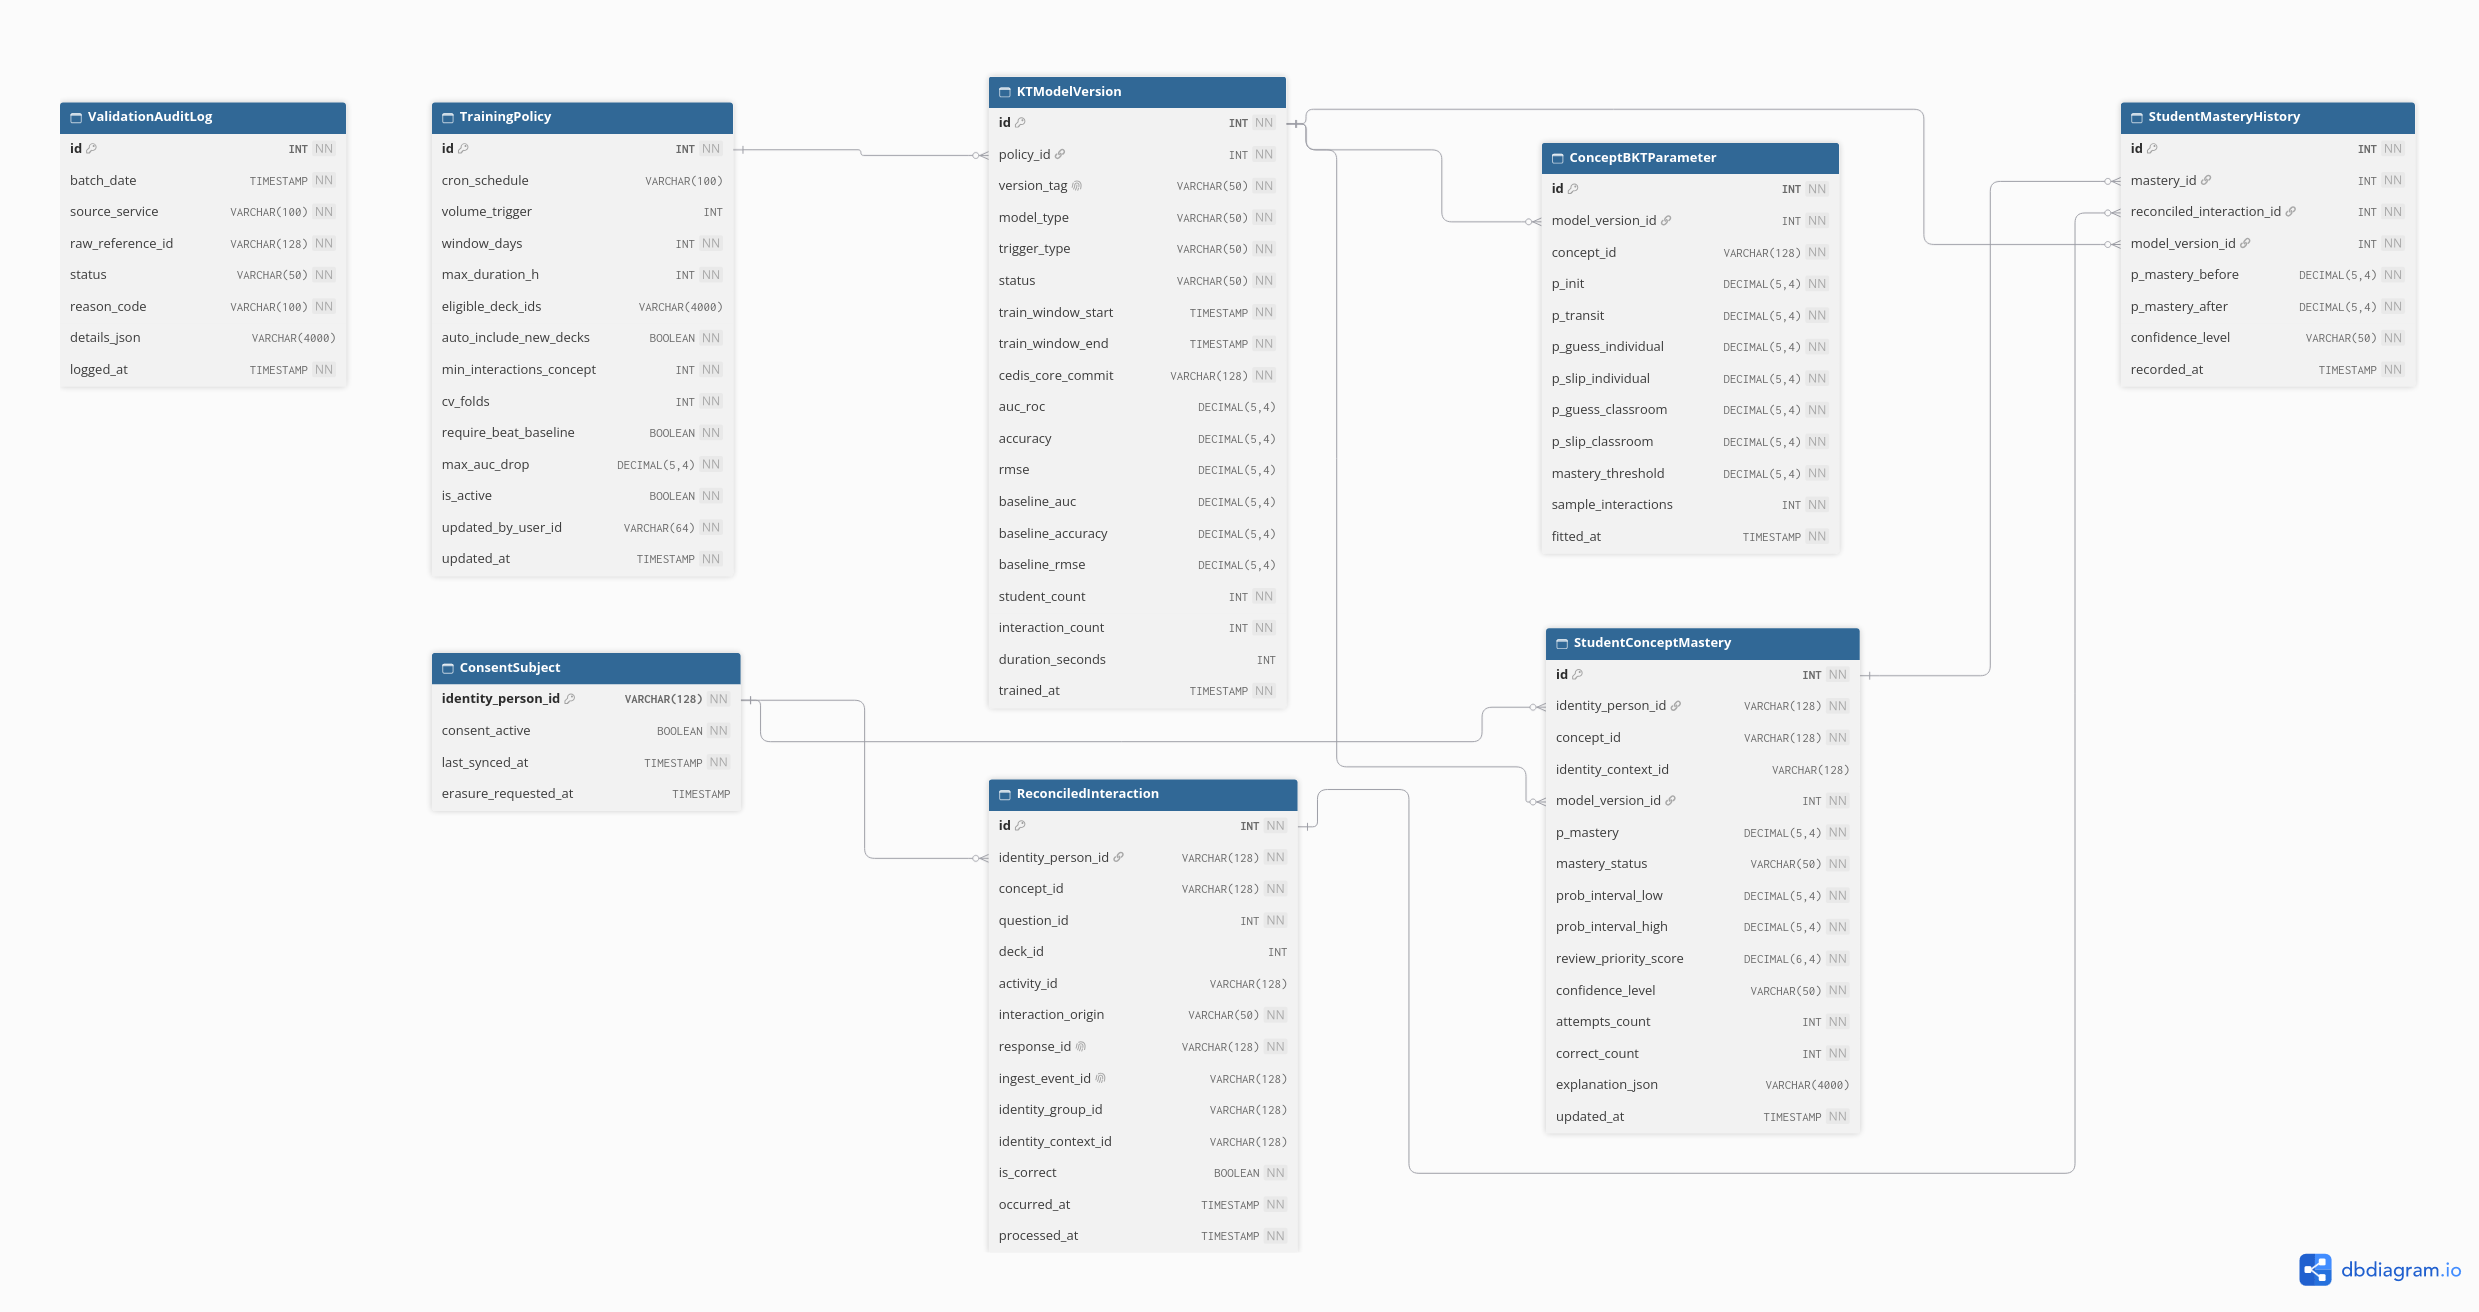
\includegraphics[width=\textwidth]{figuras/ModeloCognita.png}
\legend{Fonte: Elaborado pelos autores.}
\end{figure}

O modelo é composto por oito tabelas, dispostas da esquerda para a direita segundo o fluxo de processamento do módulo. À esquerda, a tabela \textit{ValidationAuditLog} registra os dados tratados e descartados na ingestão. Na parte superior, encadeiam-se as tabelas do modelo preditivo: cada política de treino (\textit{TrainingPolicy}) gera versões do modelo (\textit{KTModelVersion}), e cada versão possui os parâmetros dos conceitos (\textit{ConceptBKTParameter}). Na parte inferior, cada estudante com consentimento (\textit{ConsentSubject}) possui as suas respostas reconciliadas (\textit{ReconciledInteraction}) e o seu estado atual de domínio em cada conceito (\textit{StudentConceptMastery}). À direita, a tabela \textit{StudentMasteryHistory} guarda a série histórica das estimativas, ligando cada atualização à resposta que a causou e à versão do modelo utilizada. A Tabela~\ref{tab:der-entidades-cognita} sintetiza as chaves, os relacionamentos e o papel funcional de cada tabela modelada para o Cognita.

{\small
\begin{longtable}{>{\raggedright\arraybackslash}p{3.4cm}>{\raggedright\arraybackslash}p{4.2cm}>{\raggedright\arraybackslash}p{6.2cm}}
\caption{Especificação das entidades do modelo de dados do módulo Cognita}
\label{tab:der-entidades-cognita} \\
\hline
\textbf{Entidade do Cognita} & \textbf{Chaves e Relacionamentos} & \textbf{Atributos e Papel Funcional} \\
\hline
\endfirsthead
\caption[]{Especificação das entidades do modelo de dados do módulo Cognita (continuação)} \\
\hline
\textbf{Entidade do Cognita} & \textbf{Chaves e Relacionamentos} & \textbf{Atributos e Papel Funcional} \\
\hline
\endhead
\hline
\multicolumn{3}{r}{\textit{Continua na próxima página}} \\
\endfoot
\hline
\multicolumn{3}{l}{Fonte: Elaborado pelos autores.} \\
\endlastfoot
\textit{TrainingPolicy} & \texttt{id} (PK); relaciona-se $1:N$ com \textit{KTModelVersion}; referência lógica ao docente/administrador (\textit{updated\_by\_user\_id}). & Armazena as regras de treinamento e a seleção de materiais configuradas no Deck Manager: agendamento (\textit{cron\_schedule}), gatilho por volume de novas respostas (\textit{volume\_trigger}), relação de \textit{decks} habilitados no treino (\textit{eligible\_deck\_ids}), inclusão automática de novos \textit{decks} (\textit{auto\_include\_new\_decks}), número mínimo de respostas para a estimação de parâmetros próprios de um conceito (\textit{min\_interactions\_concept}), número de partições da validação cruzada (\textit{cv\_folds}), tempo limite de 6 horas (\textit{max\_duration\_h}) e critérios do \textit{Quality Gate}: exigência de superar o modelo de referência em AUC e RMSE (\textit{require\_beat\_baseline}) e queda máxima de AUC de $0{,}01$ em relação ao modelo vigente (\textit{max\_auc\_drop}). \\
\hline
\textit{KTModelVersion} & \texttt{id} (PK), \textit{version\_tag} (UQ), \textit{policy\_id} (FK); relaciona-se $1:N$ com \textit{ConceptBKTParameter}, \textit{StudentConceptMastery} e \textit{StudentMasteryHistory}. & Registra cada execução do histórico de treinos do modelo BKT: versão (ex.: \texttt{v12}), tipo de gatilho (\texttt{SCHEDULED} ou \texttt{VOLUME}), estado (\texttt{ACTIVE}, \texttt{CANDIDATE} ou \texttt{FAILED} para retenção de \textit{fallback}), período dos dados de treino, \textit{commit} do \textit{cedis-core}, métricas médias da validação cruzada do modelo (\textit{auc\_roc}, \textit{accuracy}, \textit{rmse}) e do modelo de referência (\textit{baseline\_auc}, \textit{baseline\_accuracy}, \textit{baseline\_rmse}), total de passaportes/respostas e duração (\textit{duration\_seconds}). \\
\hline
\textit{ConceptBKT\allowbreak Parameter} & \texttt{id} (PK), \textit{model\_version\_id} (FK); referência lógica a \textit{concept\_id} (\textit{cedis-atlas}); unicidade por par (versão, conceito). & Mantém os quatro parâmetros probabilísticos estimados por conceito na respectiva versão do modelo: conhecimento inicial $P(L_0)$ (\textit{p\_init}), aprendizado $P(T)$ (\textit{p\_transit}), chute $P(G) < 0{,}5$ e descuido $P(S) < 0{,}5$, estimados separadamente para os questionários individuais (\textit{p\_guess\_individual} e \textit{p\_slip\_individual}) e para as atividades em sala de aula (\textit{p\_guess\_classroom} e \textit{p\_slip\_classroom}), além do limiar de domínio (\textit{mastery\_threshold} $= 0{,}80$) e amostra de respostas utilizada no ajuste. \\
\hline
\textit{ValidationAudit\allowbreak Log} & \texttt{id} (PK); indexado por lote (\textit{batch\_date}), serviço de origem (\textit{source\_service}) e referência bruta (\textit{raw\_reference\_id}). & Registra 100\% das ocorrências de saneamento (\texttt{TREATED}, como deduplicação de \textit{activity\_submitted} repetido, reordenação de horário e reconciliação via \textit{LearningAnalyticsIngestLink}) ou descarte (\texttt{DISCARDED}, como ausência de vínculo em \textit{QuestionActivityMap}), permitindo auditoria na tela de qualidade de dados e exportação em CSV. \\
\hline
\textit{ConsentSubject} & \textit{identity\_person\_id} (PK lógica oriunda do Learning Passport); relaciona-se $1:N$ com \textit{ReconciledInteraction} e \textit{StudentConceptMastery} com \texttt{ON DELETE CASCADE}. & Entidade âncora de governança LGPD que representa o passaporte pseudonimizado com autorização ativa para o Cognita (\textit{consent\_active}). A exclusão de um registro nesta tabela propaga o expurgo físico imediato, em cascata, apenas dos dados preditivos e históricos no Cognita, preservando os demais dados do aluno no ecossistema. \\
\hline
\textit{Reconciled\allowbreak Interaction} & \texttt{id} (PK), \textit{identity\_person\_id} (FK \texttt{CASCADE}), \textit{response\_id} (UQ lógico), \textit{ingest\_event\_id} (UQ lógico); relaciona-se $1:N$ com \textit{StudentMasteryHistory}. & Materializa a resposta validada de um \textit{deck} elegível ou prática do Atlas associada à Matriz Q (\textit{question\_id} e \textit{concept\_id}), registrando o resultado binário $a_t \in \{0, 1\}$ (\textit{is\_correct}), a origem (\textit{interaction\_origin}: CEDIS Slides, prática de fixação ou expedição do Atlas), o curso/turma (\textit{identity\_context\_id}) e o instante em UTC. \\
\hline
\textit{StudentConcept\allowbreak Mastery} & \texttt{id} (PK), \textit{identity\_person\_id} (FK \texttt{CASCADE}), \textit{model\_version\_id} (FK); unicidade por (estudante, conceito, contexto); relaciona-se $1:N$ com \textit{StudentMasteryHistory}. & Representa o estado cognitivo atual do estudante em cada conceito: probabilidade $P(L_t)$ (\textit{p\_mastery}), situação (\textit{mastery\_status}: dominado $\ge 80\%$, em progresso $50\%$ a $79\%$, a revisar $< 50\%$ ou sem evidências), faixa provável (\textit{prob\_interval\_low/high}), prioridade de revisão ponderada por pré-requisitos (\textit{review\_priority\_score}), confiança (\textit{alta} $\ge 8$, \textit{média} $3$ a $7$, \textit{baixa} $\le 2$ evidências), contadores de tentativas/acertos e motivos em JSON (\textit{explanation\_json}). \\
\hline
\textit{StudentMastery\allowbreak History} & \texttt{id} (PK), \textit{mastery\_id} (FK \texttt{CASCADE}), \textit{reconciled\_interaction\_id} (FK), \textit{model\_version\_id} (FK). & Armazena a série temporal longitudinal das estimativas a cada resposta processada, registrando a probabilidade anterior $P(L_t)$ (\textit{p\_mastery\_before}), a probabilidade atualizada $P(L_{t+1})$ (\textit{p\_mastery\_after}), a confiança e a data em UTC (\textit{recorded\_at}), alimentando o gráfico individual no Atlas, o quadro pós-prática no Slides e a evolução semanal da turma no Analytics. \\
\hline
\end{longtable}
}

Três decisões de projeto desse modelo merecem destaque:
\begin{enumerate}
    \item \textbf{Exclusão em cascata (LGPD):} o identificador pseudonimizado do passaporte fica centralizado em \textit{ConsentSubject}, e as tabelas dependentes são removidas em cascata (\texttt{ON DELETE CASCADE}). Assim, a exclusão dos dados preditivos de um estudante é feita por uma única operação, sem deixar registros órfãos, o que permite cumprir o prazo de 48 horas (RNF16);
    \item \textbf{Separação entre estado atual e histórico:} \textit{StudentConceptMastery} mantém apenas um registro por estudante, conceito e contexto, com os valores já calculados, enquanto \textit{StudentMasteryHistory} acumula a evolução a cada resposta. Assim, as consultas frequentes do estudante e as agregações do docente não precisam percorrer o histórico, o que contribui para os tempos de resposta dos RNF08 e RNF09;
    \item \textbf{Versionamento do modelo:} como os parâmetros e as estimativas estão ligados à versão do modelo (\textit{model\_version\_id}), a versão em operação (\texttt{ACTIVE}) e uma versão candidata (\texttt{CANDIDATE}) podem coexistir durante o retreinamento. Se a candidata falhar ou for reprovada pelo \textit{Quality Gate}, ela é marcada como \texttt{FAILED}, e as consultas continuam a usar a versão anterior, sem interrupção do serviço (RNF06).
\end{enumerate}


\section{Prototipação das Telas}
\label{sec:prototipacao}

Com os requisitos definidos e priorizados, foram elaborados protótipos de alta fidelidade das telas do Cognita, com o objetivo de validar, antes da implementação, como as estimativas de domínio serão apresentadas ao estudante e ao professor. Como o Cognita é um módulo integrado ao ecossistema, e não um novo software, os protótipos não descrevem uma aplicação própria: eles mostram como as funcionalidades do módulo aparecem dentro das aplicações já existentes do CEDIS, que são o Atlas, o CEDIS Slides, o Learning Analytics, o Concept Studio, o Deck Manager e o Learning Passport.

Cada tela foi desenhada a partir de um conjunto de requisitos funcionais do MVP, indicados na legenda de cada figura, de modo que todos os requisitos do MVP estão representados em pelo menos uma tela. Os requisitos dos incrementos (RF14, RF21, RF22, RF23 e RF25) não foram prototipados, pois não serão entregues no desenvolvimento. Para manter a coerência entre as telas, todos os protótipos utilizam um mesmo cenário fictício: a disciplina de Compiladores, ministrada por uma professora, e um estudante identificado apenas pelo pseudônimo do seu passaporte.

\subsection{Telas do Estudante}
\label{subsec:prototipo-estudante}

A principal tela do estudante é a página \textit{Seu domínio}, no Atlas, apresentada na Figura~\ref{fig:prototipo-atlas-dominio}. Nela, o estudante escolhe um curso e visualiza a probabilidade de domínio de cada conceito (RF06), agrupada em quatro situações: dominado (probabilidade igual ou superior a 80\%), em progresso, a revisar e sem evidências. A seção \textit{Revise primeiro} lista os conceitos ainda não dominados em ordem de prioridade de revisão (RF08), considerando tanto o menor domínio quanto os conceitos que servem de base para os próximos destinos da rota. Cada estimativa é acompanhada do seu grau de confiança e da quantidade de evidências que a sustentam (RF16), e o indicador de atualização informa que a página reflete a interação mais recente do estudante (RF07). O texto da tela reforça que as estimativas são orientações e não bloqueiam a rota nem valem nota.

\begin{figure}[H]
\caption{Protótipo da página \textit{Seu domínio} no Atlas (RF06, RF07, RF08 e RF16)}
\label{fig:prototipo-atlas-dominio}
\centering
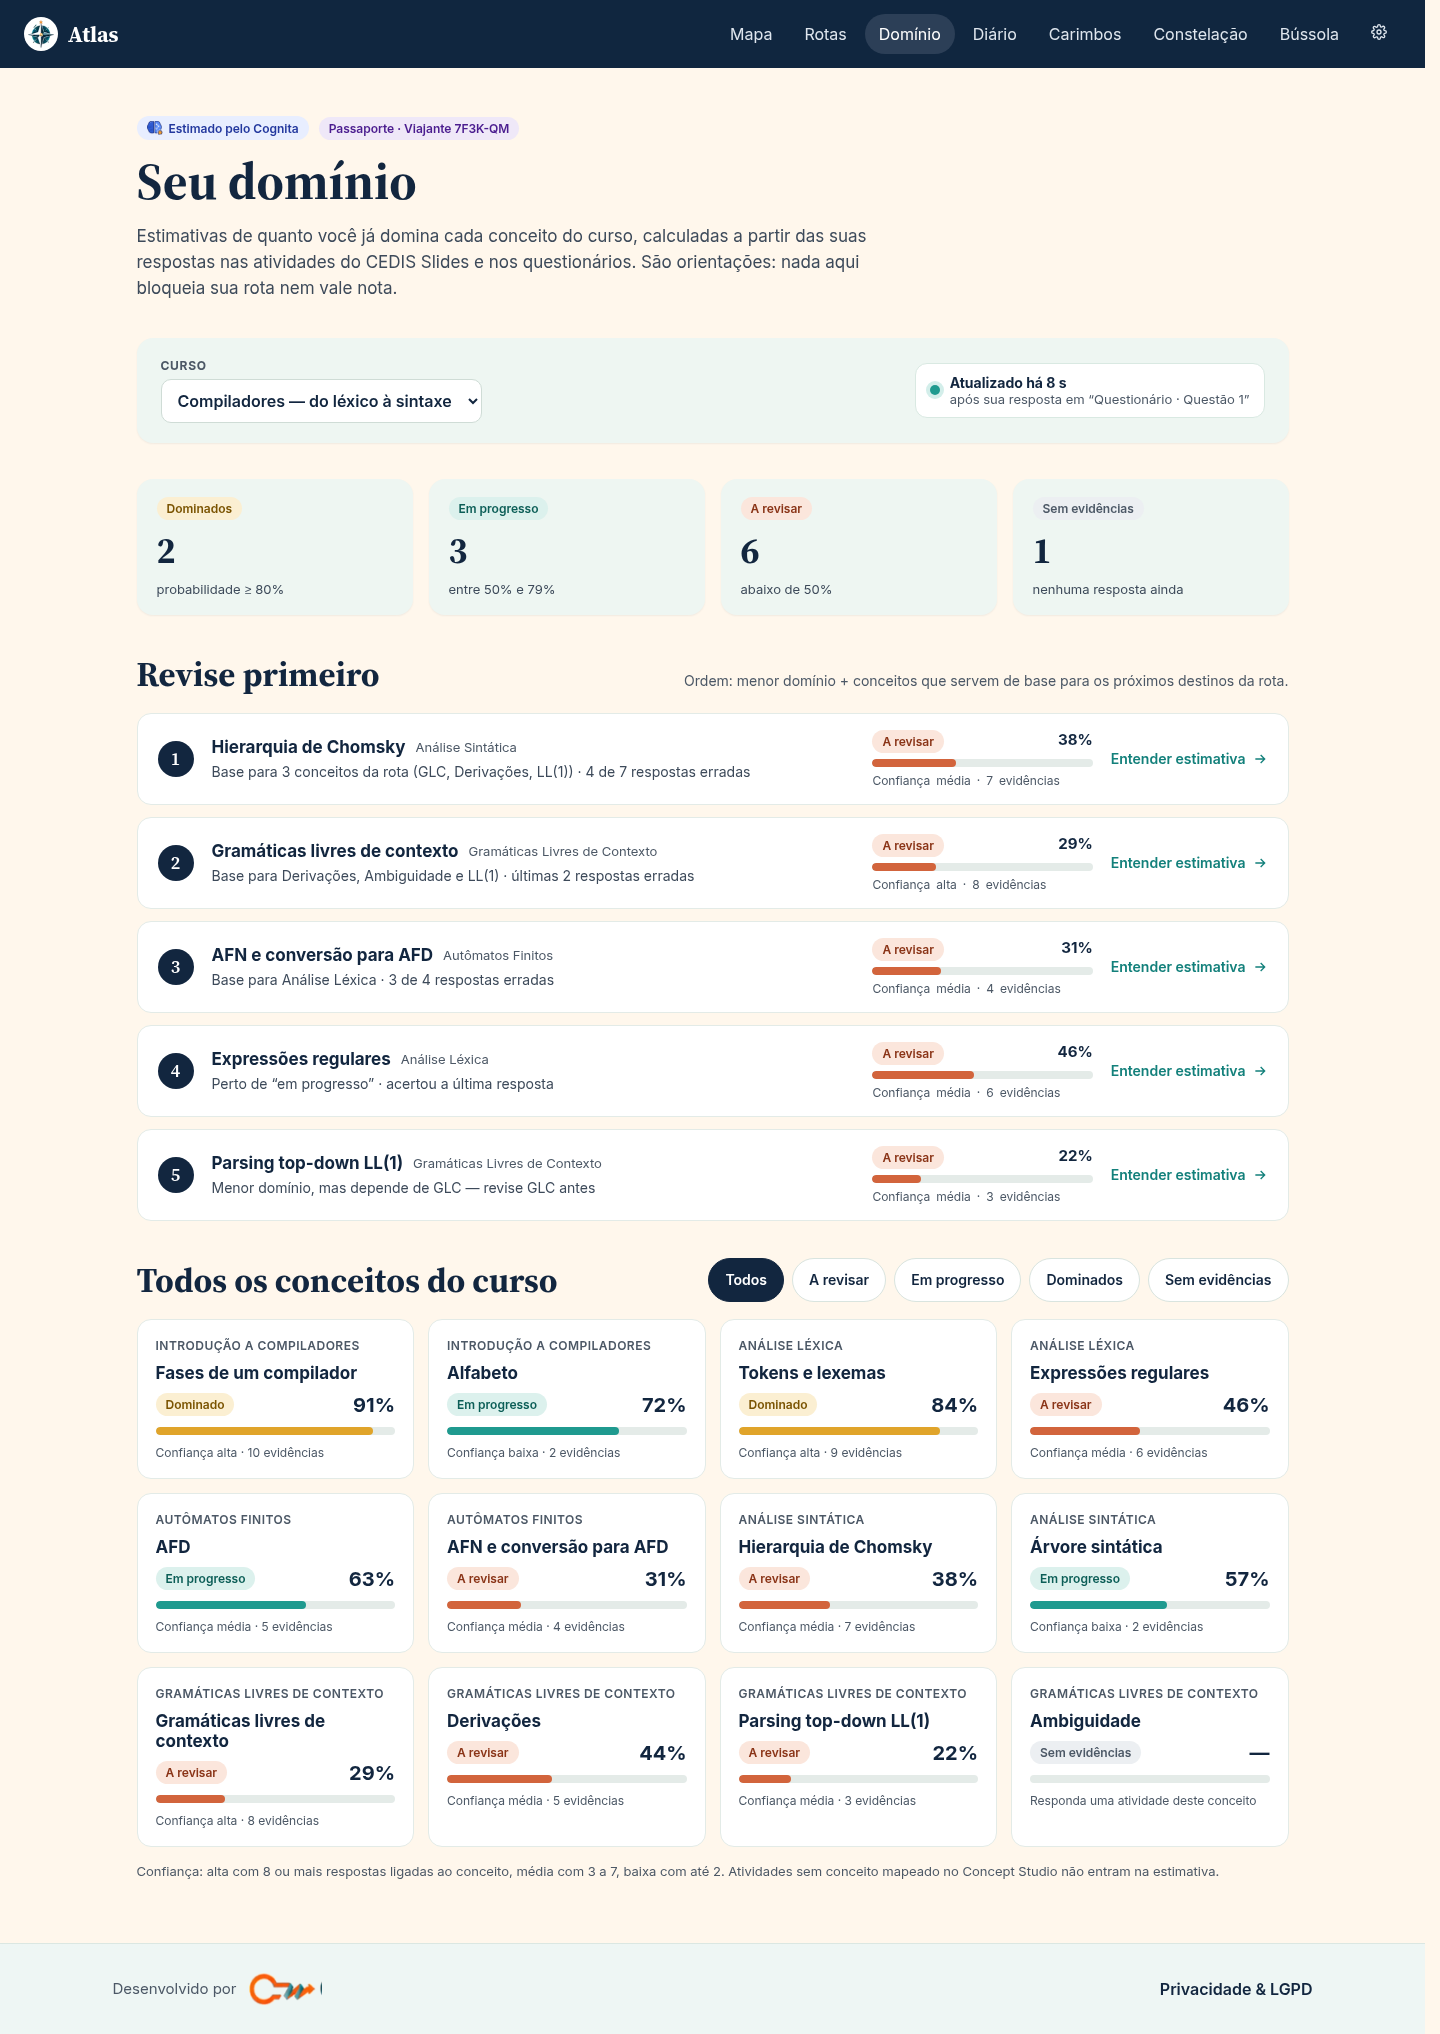
\includegraphics[width=\textwidth,height=0.72\textheight,keepaspectratio]{figuras/prototipo/atlas-seu-dominio-rf06-rf07-rf08-rf16.png}
\legend{Fonte: Elaborado pelos autores.}
\end{figure}

Ao selecionar a opção \textit{Entender estimativa}, o estudante acessa o detalhe do conceito, apresentado na Figura~\ref{fig:prototipo-atlas-detalhe}. A tela mostra a probabilidade de domínio atual e a última variação causada por uma resposta (RF07), além de um quadro que explica o quanto confiar na estimativa e qual é a sua faixa provável (RF16). O bloco \textit{Por que 38\%?} descreve, em linguagem acessível, os motivos que levaram à estimativa, como a quantidade de acertos e erros, o peso das respostas mais recentes e a origem das atividades (RF17). Por fim, o gráfico \textit{Seu histórico neste conceito} exibe a evolução da estimativa ao longo do tempo, com cada ponto correspondendo a uma resposta do estudante (RF09).

\begin{figure}[H]
\caption{Protótipo do detalhe de um conceito no Atlas (RF07, RF09, RF16 e RF17)}
\label{fig:prototipo-atlas-detalhe}
\centering
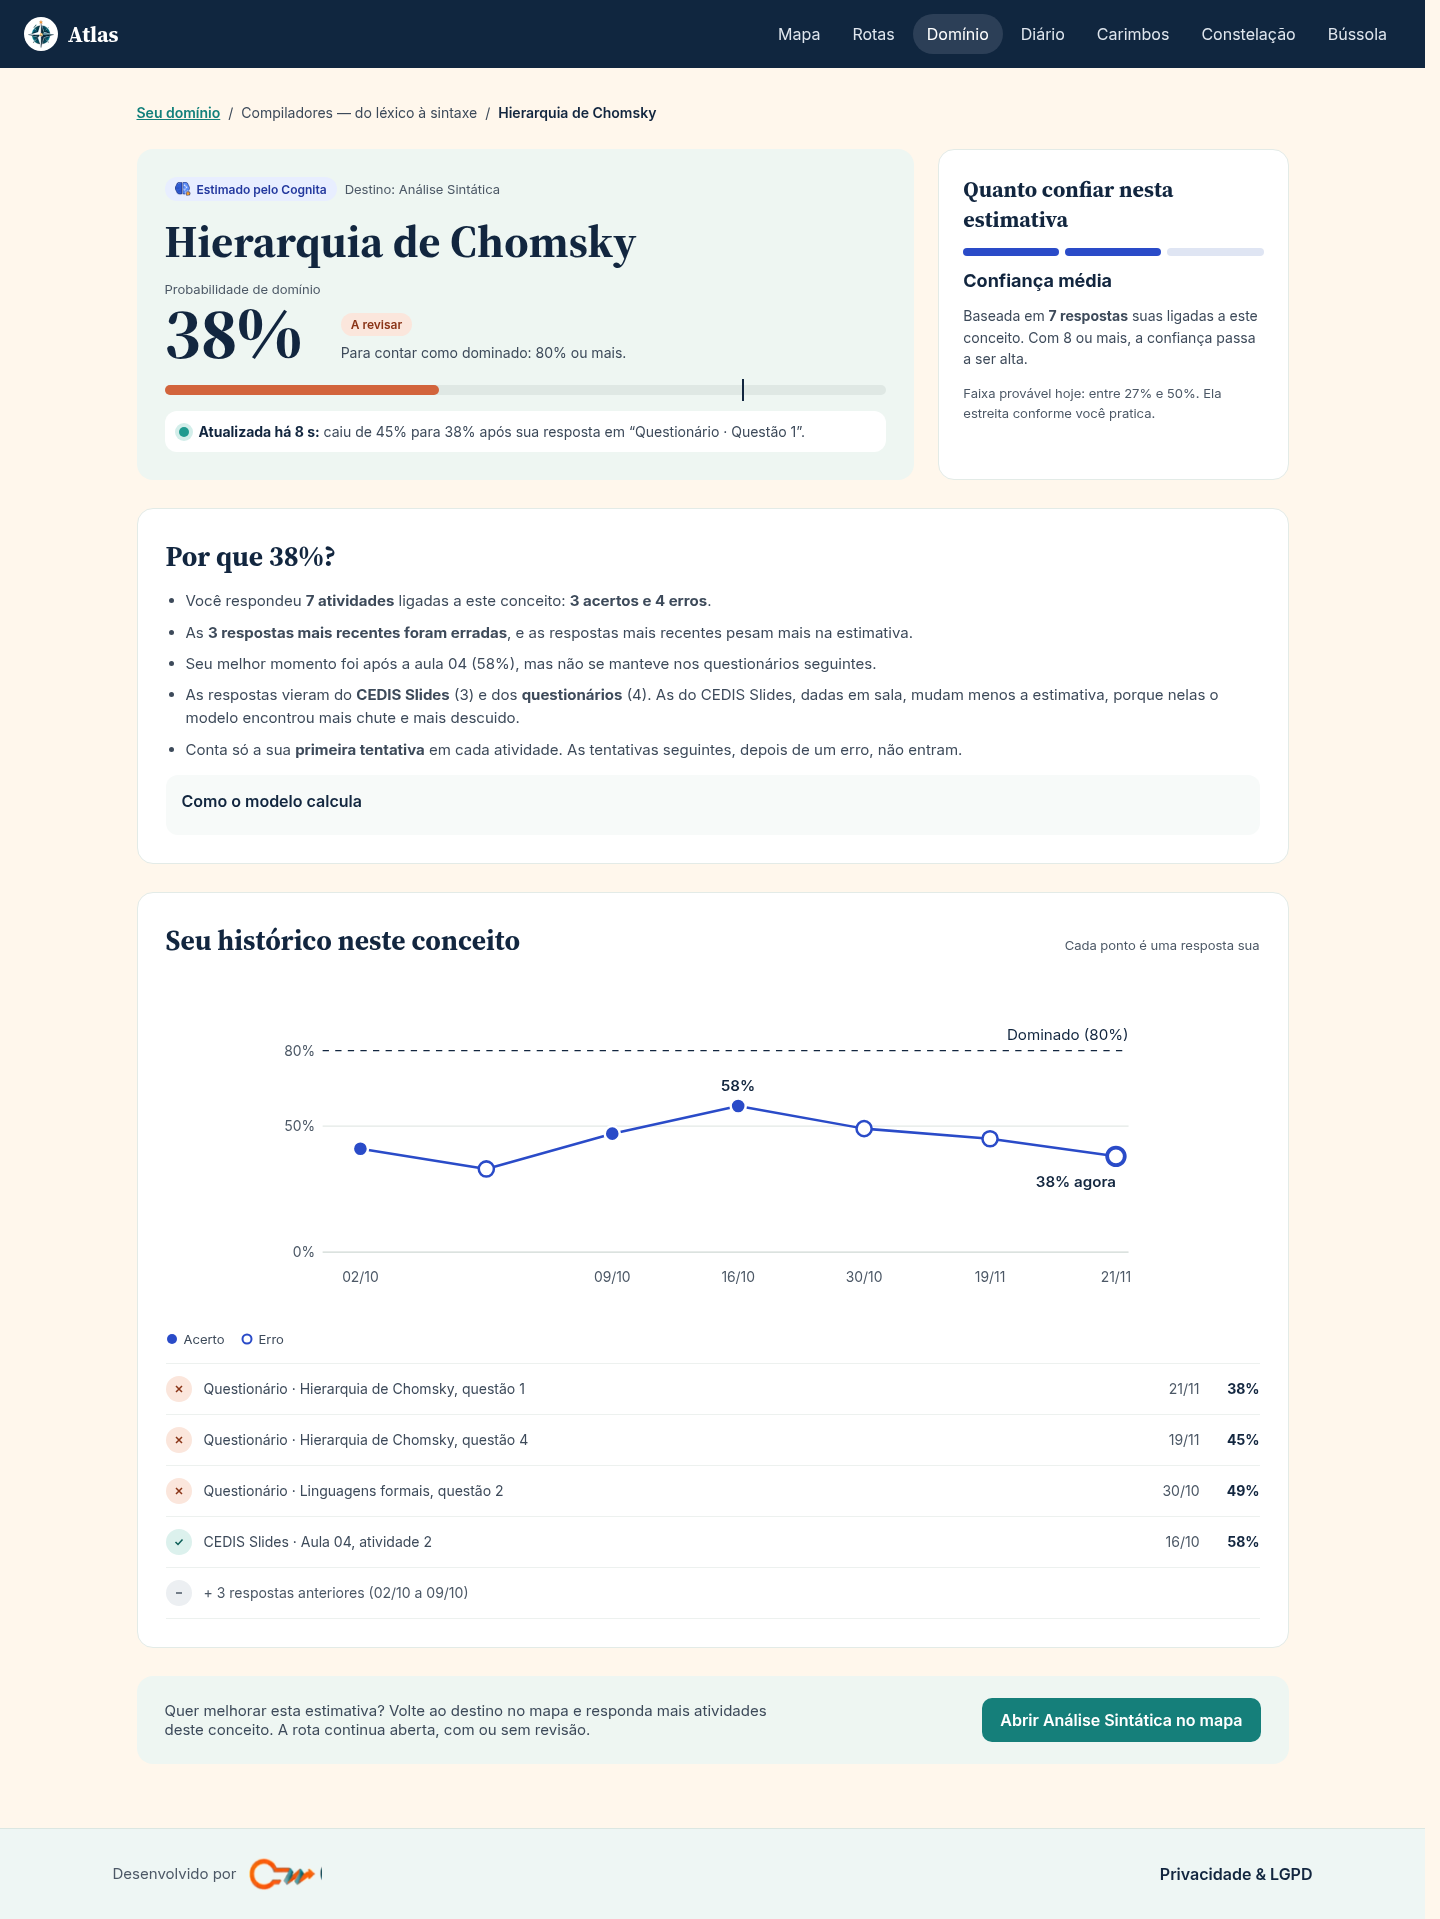
\includegraphics[width=\textwidth,height=0.72\textheight,keepaspectratio]{figuras/prototipo/atlas-detalhe-conceito-rf07-rf09-rf16-rf17.png}
\legend{Fonte: Elaborado pelos autores.}
\end{figure}

A atualização das estimativas também é percebida fora do Atlas. A Figura~\ref{fig:prototipo-slides} mostra uma questão de prática no CEDIS Slides: após o envio da resposta, um quadro informa como o domínio dos conceitos ligados à questão foi alterado (RF07) e oferece um atalho para a página \textit{Seu domínio}. O quadro só é exibido quando o Learning Passport do estudante está ativo e com o Cognita autorizado.

\begin{figure}[H]
\caption{Protótipo da atualização da estimativa após uma prática no CEDIS Slides (RF07)}
\label{fig:prototipo-slides}
\centering
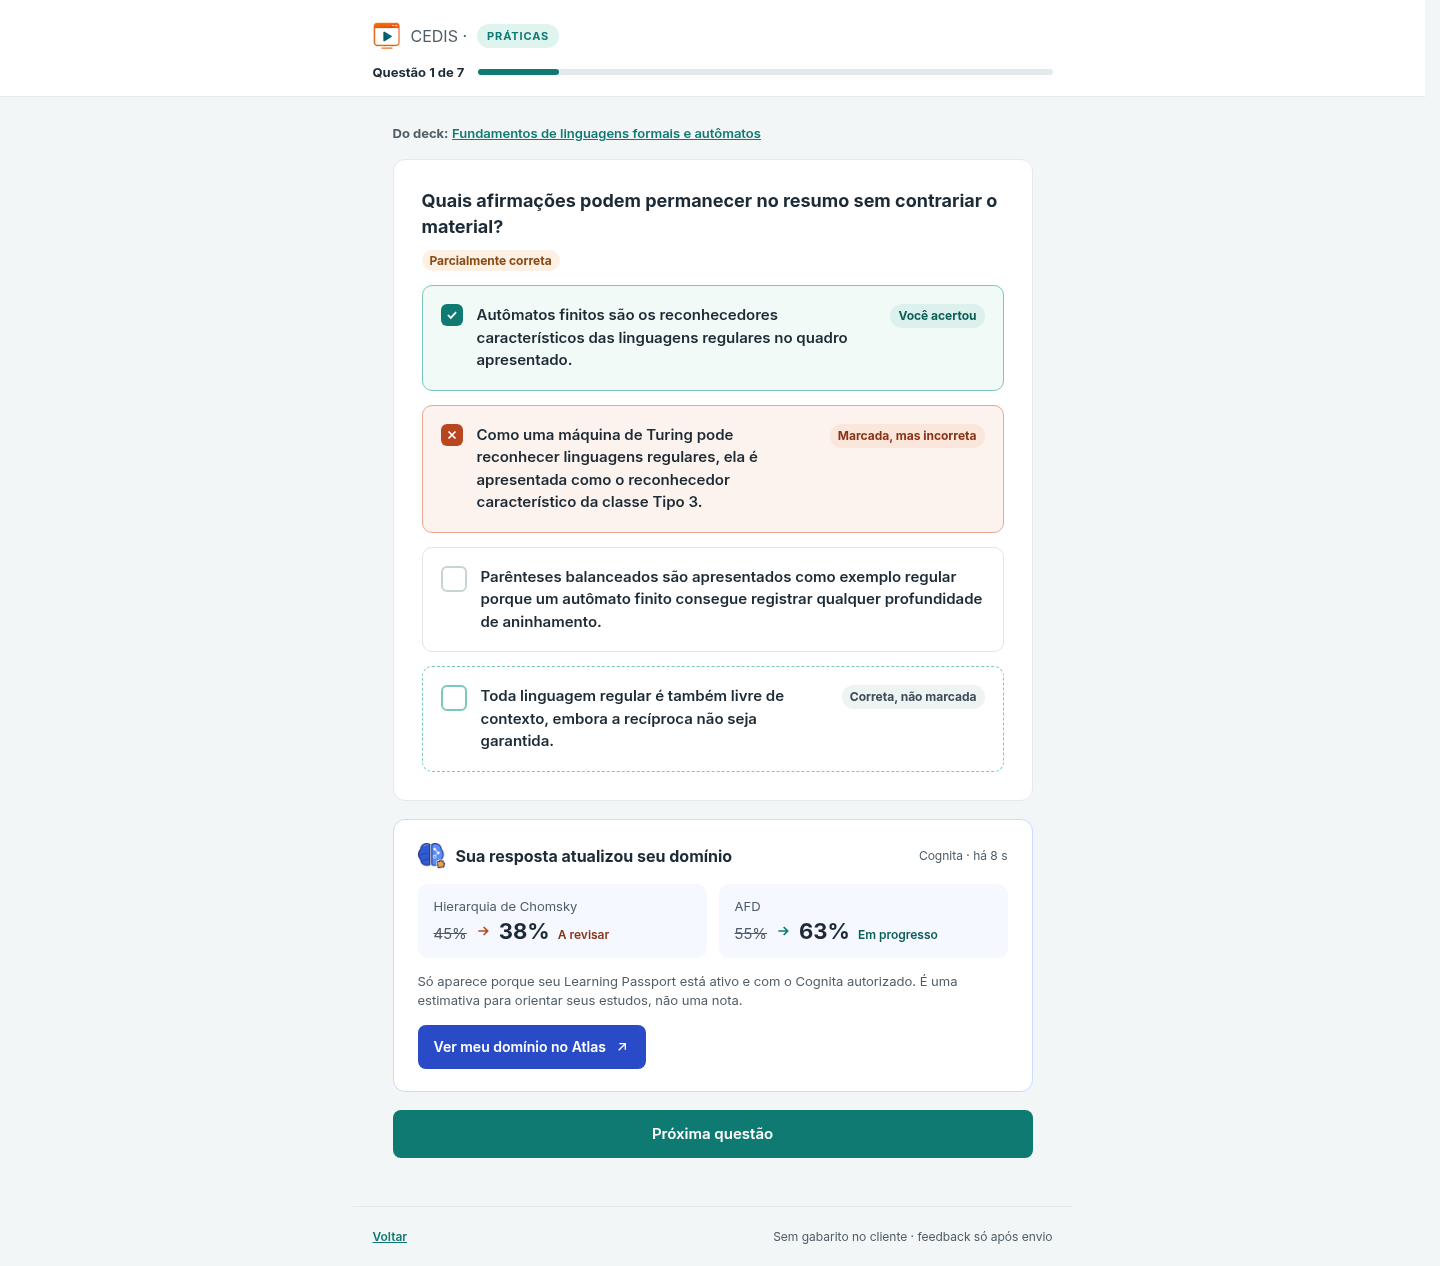
\includegraphics[width=0.85\textwidth,height=0.72\textheight,keepaspectratio]{figuras/prototipo/slides-pratica-enviada-rf07.png}
\legend{Fonte: Elaborado pelos autores.}
\end{figure}

\subsection{Telas do Professor}
\label{subsec:prototipo-professor}

No Learning Analytics, o Cognita é apresentado na aba \textit{Domínio da turma por conceito}, ilustrada na Figura~\ref{fig:prototipo-analytics-turma}. A tela exibe a proporção estimada de estudantes que dominam cada conceito do curso (RF11), com os conceitos ordenados do menor ao maior nível de absorção (RF13) e sinalizados quando a absorção é baixa (RF12). Os filtros por curso, turma, período e conceito permitem concentrar a análise nos grupos de interesse (RF15), e cada linha apresenta o intervalo provável, a quantidade de estudantes envolvidos e o grau de confiança da estimativa (RF18). Conceitos com menos de cinco estudantes têm o indicador suprimido, conforme o RNF15. Na parte inferior, o quadro \textit{Qualidade do modelo} resume as métricas AUC, acurácia e RMSE do modelo em uso (RF05), comparando-as com os limites definidos no RNF05.

\begin{figure}[H]
\caption{Protótipo do domínio da turma por conceito no Learning Analytics (RF05, RF11, RF12, RF13, RF15 e RF18)}
\label{fig:prototipo-analytics-turma}
\centering
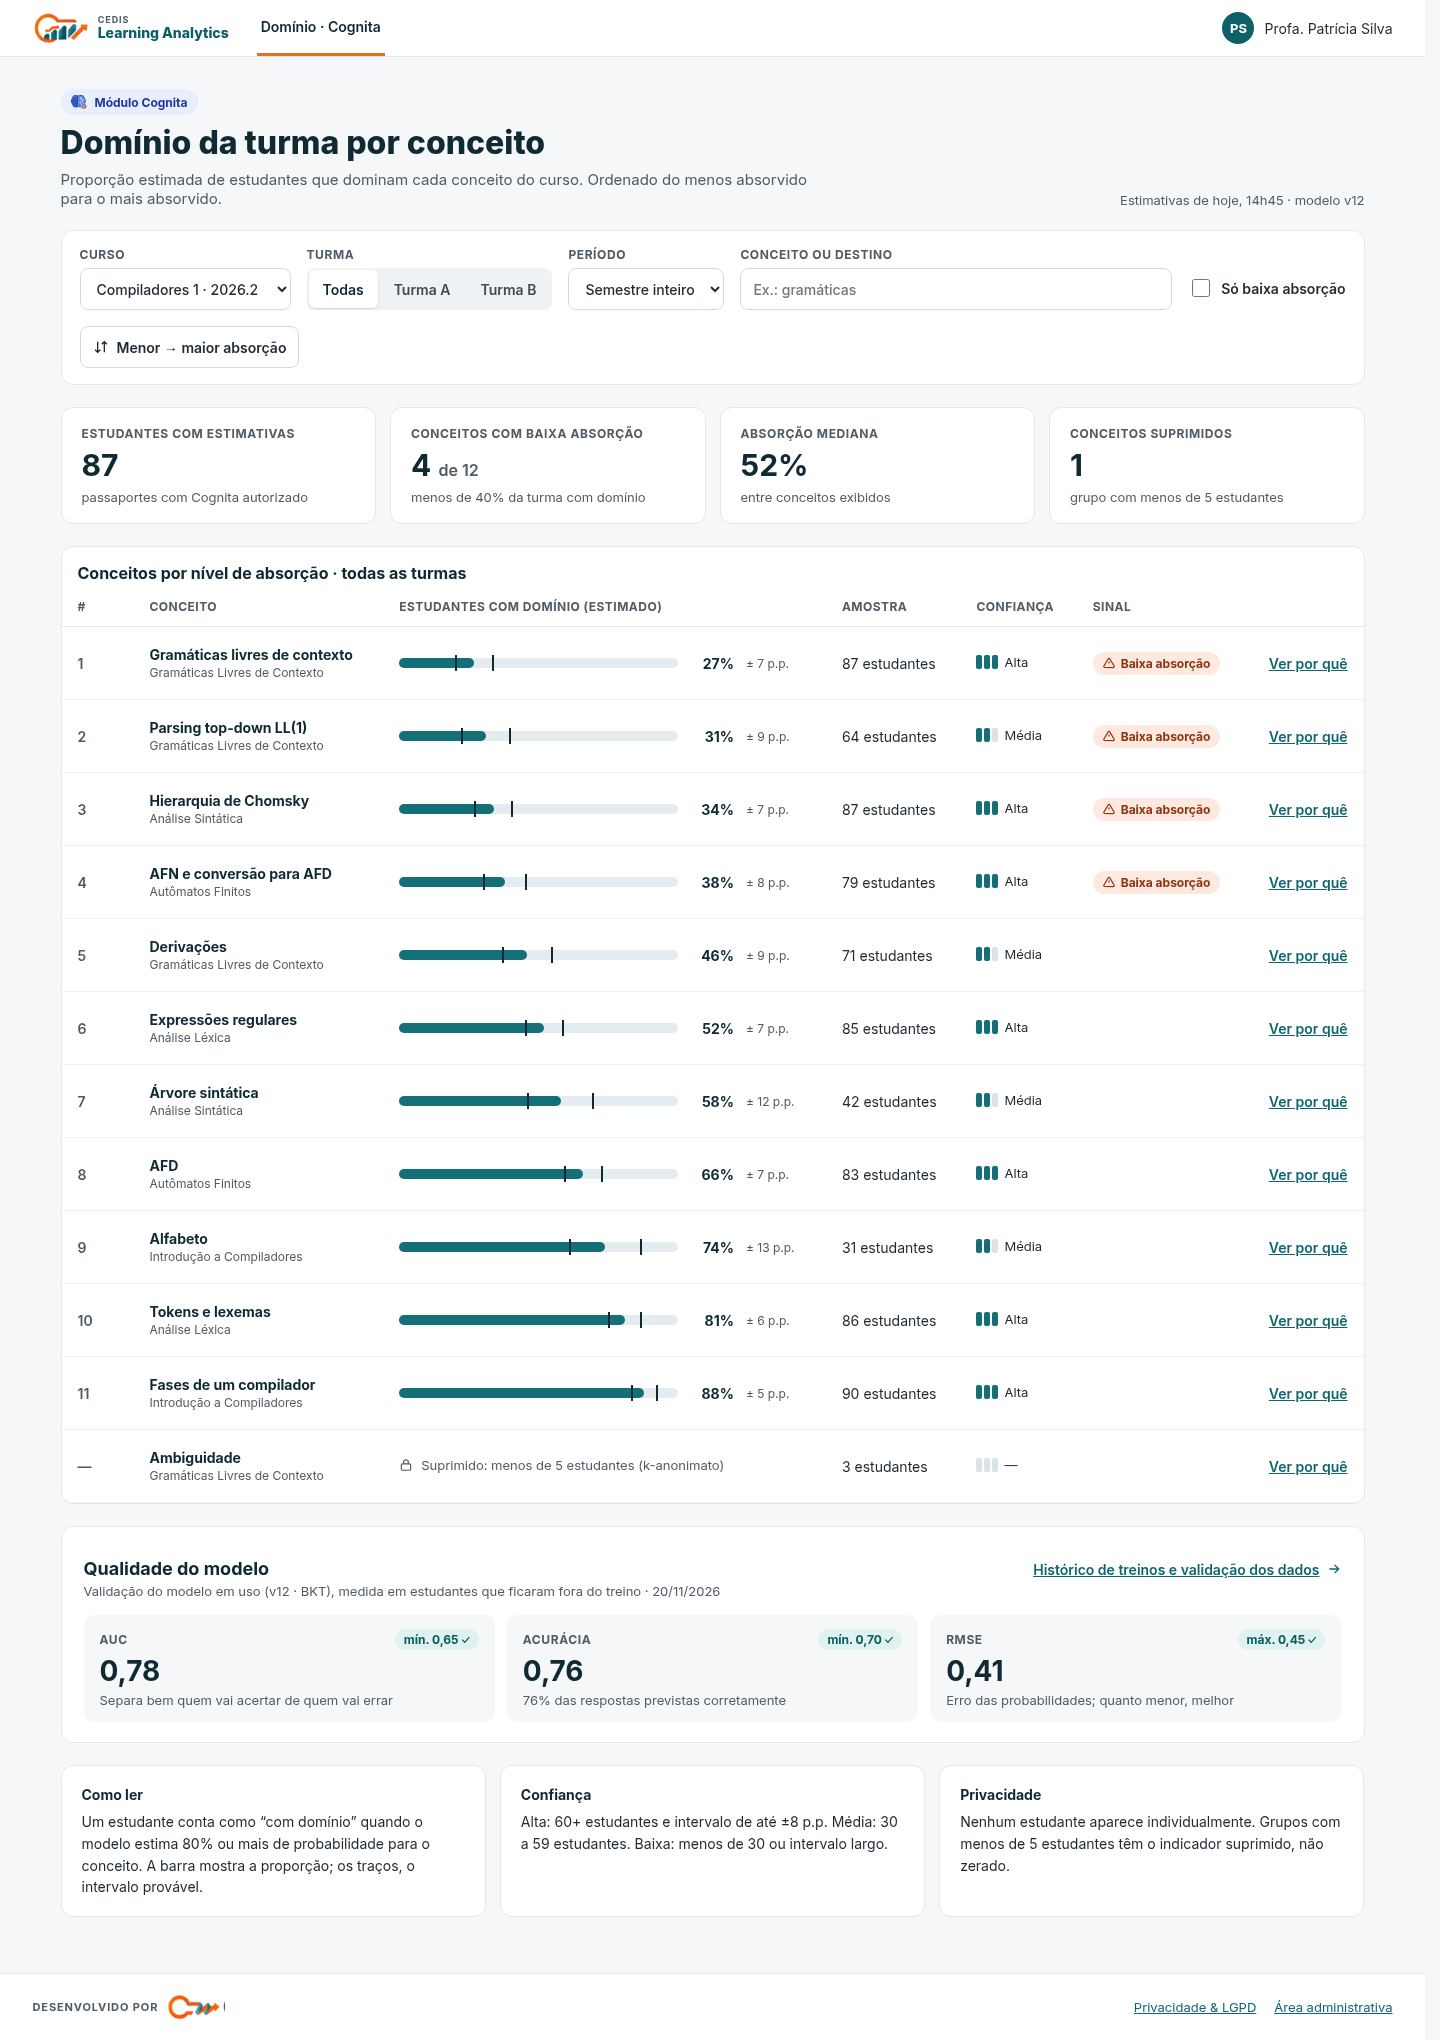
\includegraphics[width=\textwidth,height=0.72\textheight,keepaspectratio]{figuras/prototipo/analytics-dominio-turma-rf05-rf11-rf12-rf13-rf15-rf18.png}
\legend{Fonte: Elaborado pelos autores.}
\end{figure}

Ao selecionar \textit{Ver por quê} em um conceito, o professor acessa a tela da Figura~\ref{fig:prototipo-analytics-conceito}. Nela, o gráfico \textit{Evolução da absorção} mostra a proporção da turma com domínio ao longo das semanas (RF10), permitindo comparar o conceito com seus pré-requisitos e dependentes e marcar eventos pedagógicos, como uma aula de revisão. O quadro superior informa a amostra, as respostas utilizadas, o intervalo provável e a confiança da estimativa (RF18), enquanto o bloco \textit{Por que o Cognita estimou 27\%?} explica os motivos da estimativa, como as questões com mais erros, a baixa absorção do pré-requisito e os parâmetros de chute e descuido estimados pelo BKT (RF19).

\begin{figure}[H]
\caption{Protótipo do detalhe de um conceito no Learning Analytics (RF10, RF18 e RF19)}
\label{fig:prototipo-analytics-conceito}
\centering
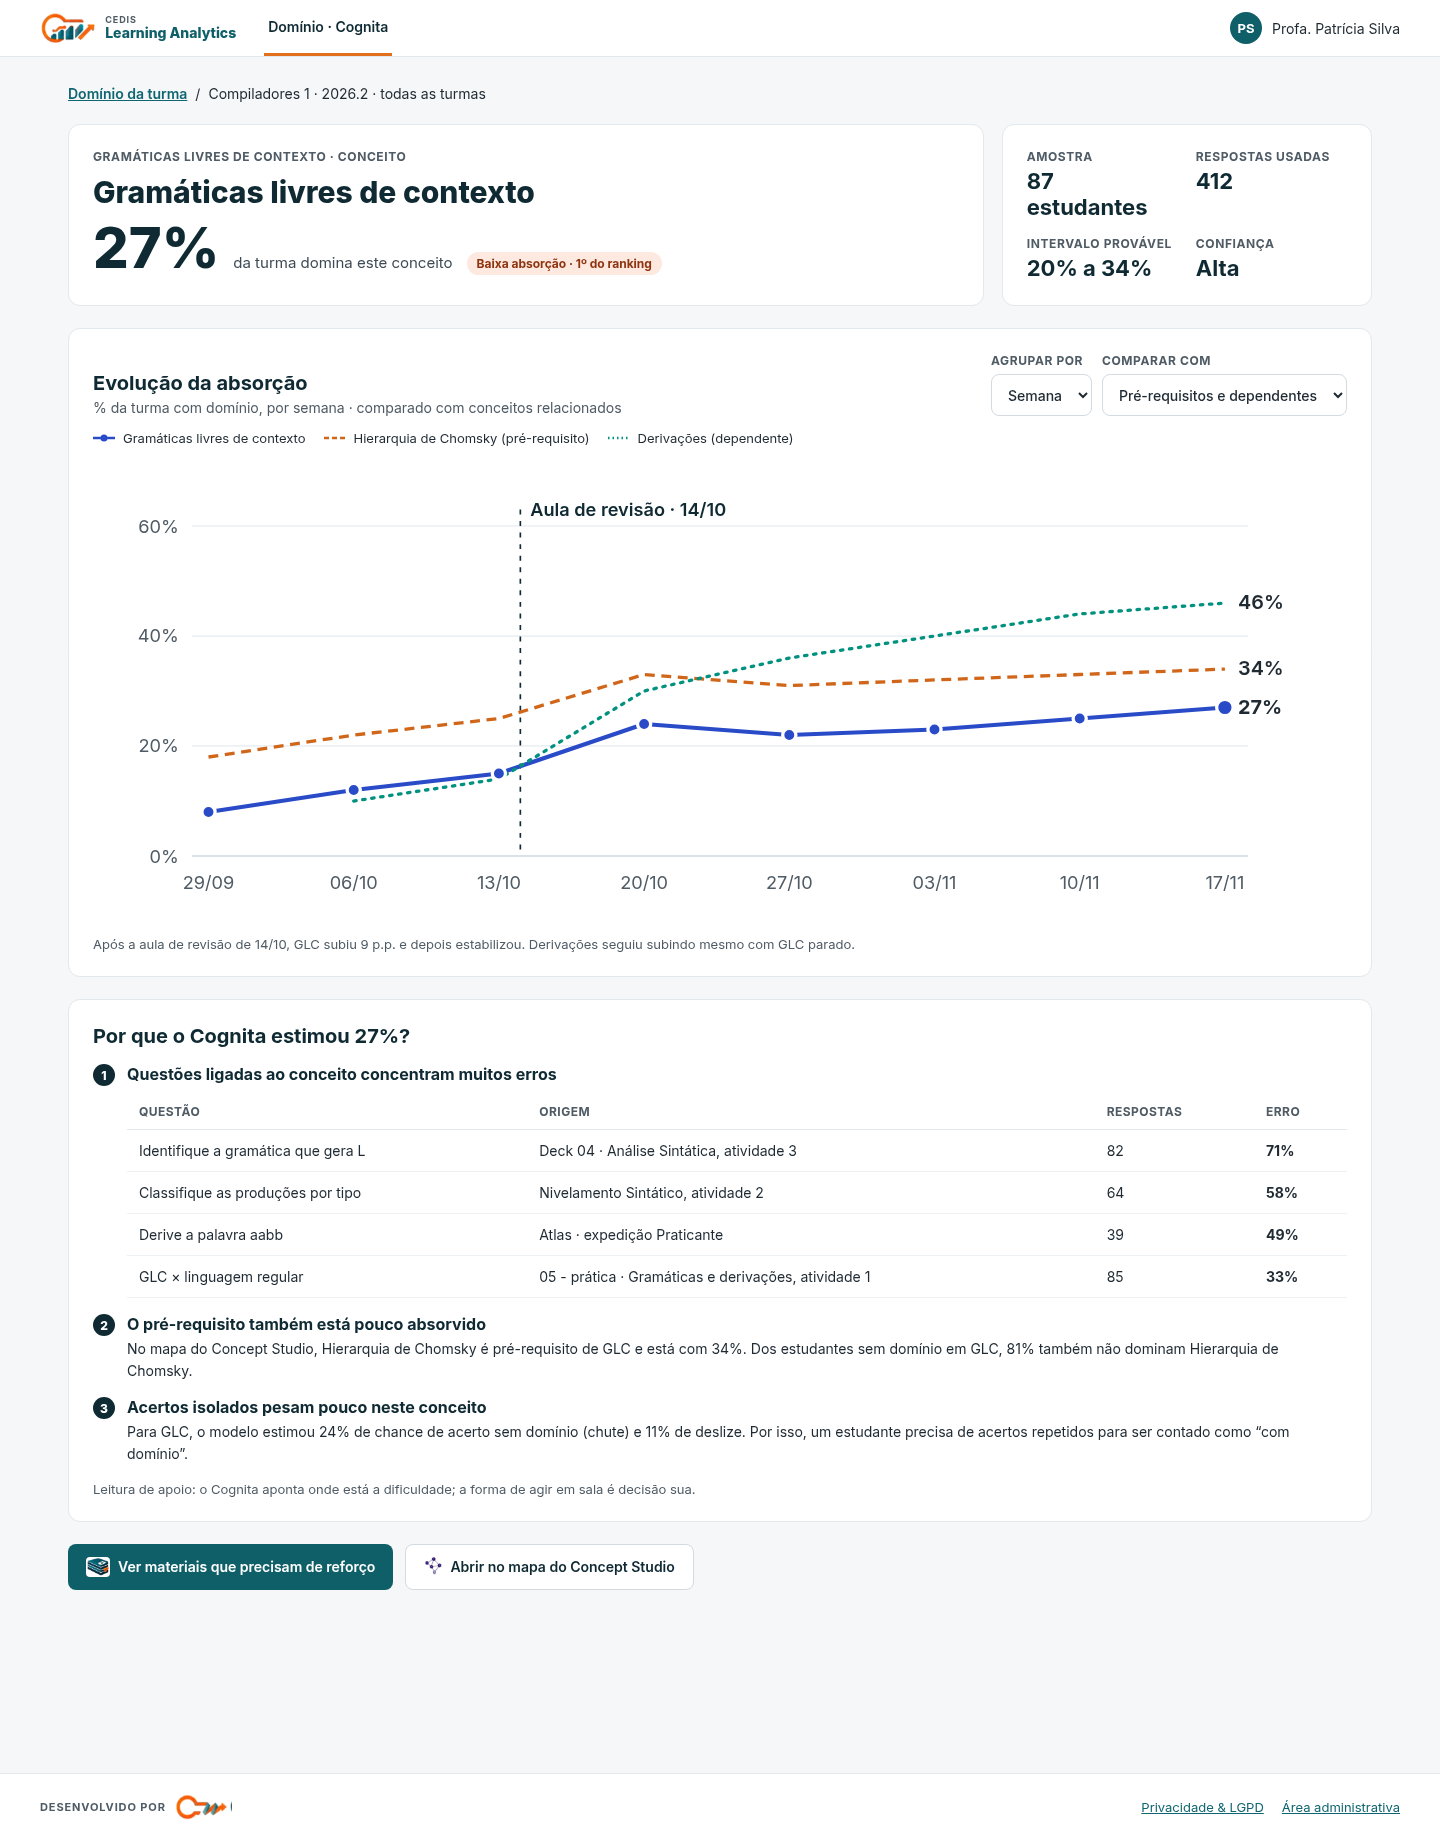
\includegraphics[width=\textwidth,height=0.72\textheight,keepaspectratio]{figuras/prototipo/analytics-conceito-rf10-rf18-rf19.png}
\legend{Fonte: Elaborado pelos autores.}
\end{figure}

A tela \textit{Modelo e qualidade dos dados}, apresentada na Figura~\ref{fig:prototipo-analytics-modelo}, reúne as informações sobre o funcionamento do modelo preditivo. O primeiro quadro identifica o modelo BKT em operação, o período dos dados de treino, os parâmetros e a divisão de teste, atendendo à rastreabilidade exigida pelo RNF13. Os gráficos e o \textit{Histórico de treinos} mostram as métricas registradas a cada treinamento (RF05) e o resultado de cada retreinamento (RF02), indicando quais versões foram promovidas e quais foram mantidas fora de operação por não atingirem os critérios definidos (RF01). Por fim, o quadro \textit{Validação dos dados recebidos} detalha quantos registros foram recebidos, tratados e descartados em cada lote, com os respectivos motivos (RF03).

\begin{figure}[H]
\caption{Protótipo do modelo e da qualidade dos dados no Learning Analytics (RF01, RF02, RF03, RF05 e RNF13)}
\label{fig:prototipo-analytics-modelo}
\centering
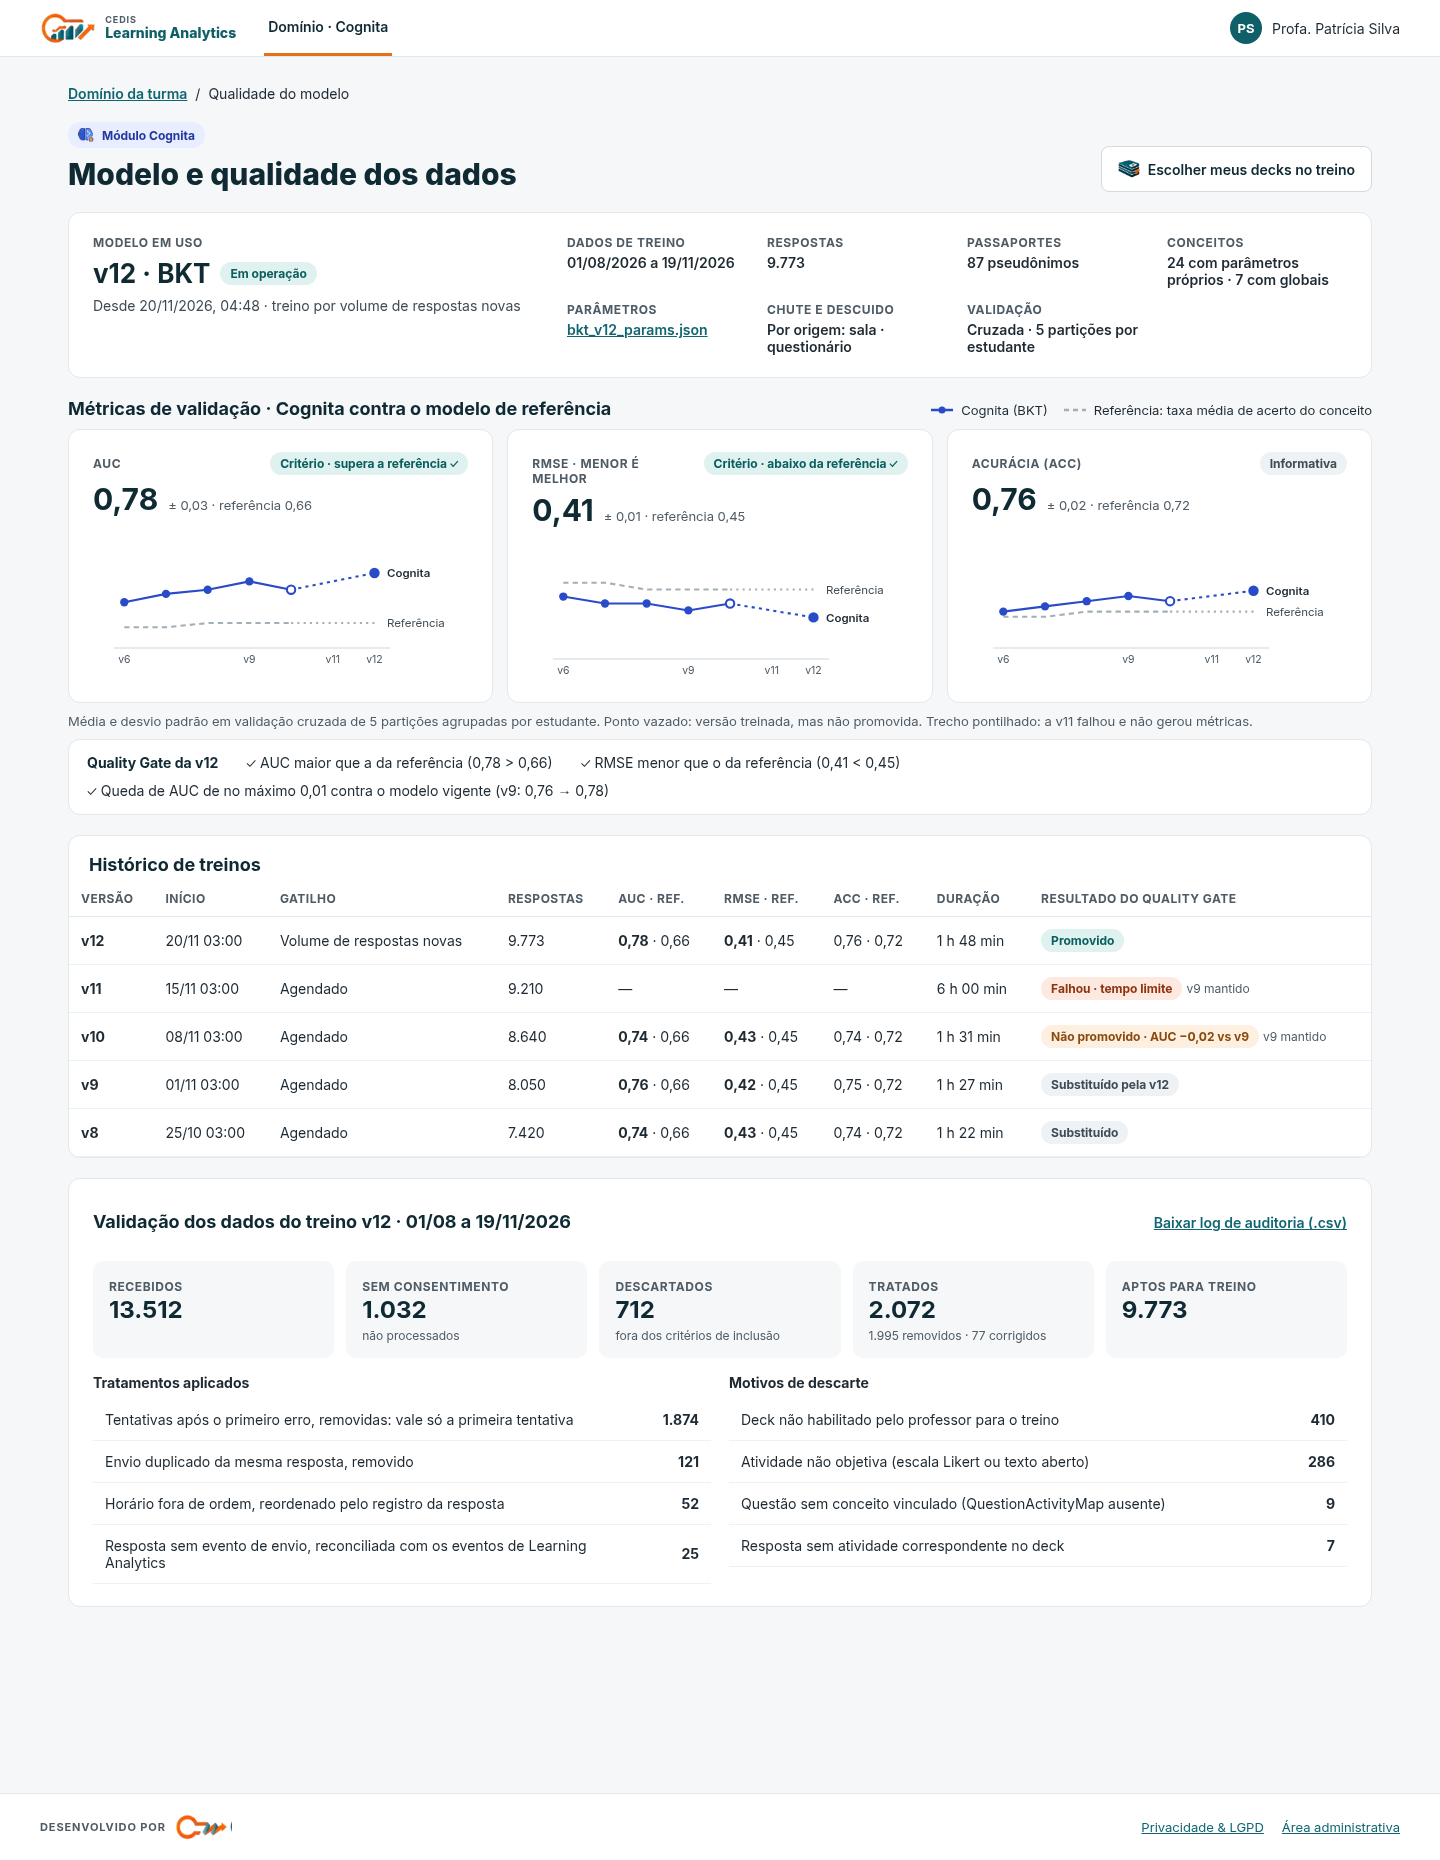
\includegraphics[width=\textwidth,height=0.72\textheight,keepaspectratio]{figuras/prototipo/analytics-qualidade-modelo-rf01-rf02-rf03-rf05-rnf13.png}
\legend{Fonte: Elaborado pelos autores.}
\end{figure}

No Concept Studio, a absorção da turma é sobreposta ao mapa conceitual do curso, como mostra a Figura~\ref{fig:prototipo-concept-studio}. Ao ativar a opção \textit{Mostrar absorção da turma}, cada conceito do mapa passa a exibir a proporção estimada de estudantes com domínio, e os conceitos com baixa absorção recebem destaque visual e são listados no painel lateral (RF12). Dessa forma, o professor identifica os conceitos críticos diretamente nas relações de pré-requisito e hierarquia que ele mesmo mapeou.

\begin{figure}[H]
\caption{Protótipo do mapa conceitual com absorção no Concept Studio (RF12)}
\label{fig:prototipo-concept-studio}
\centering
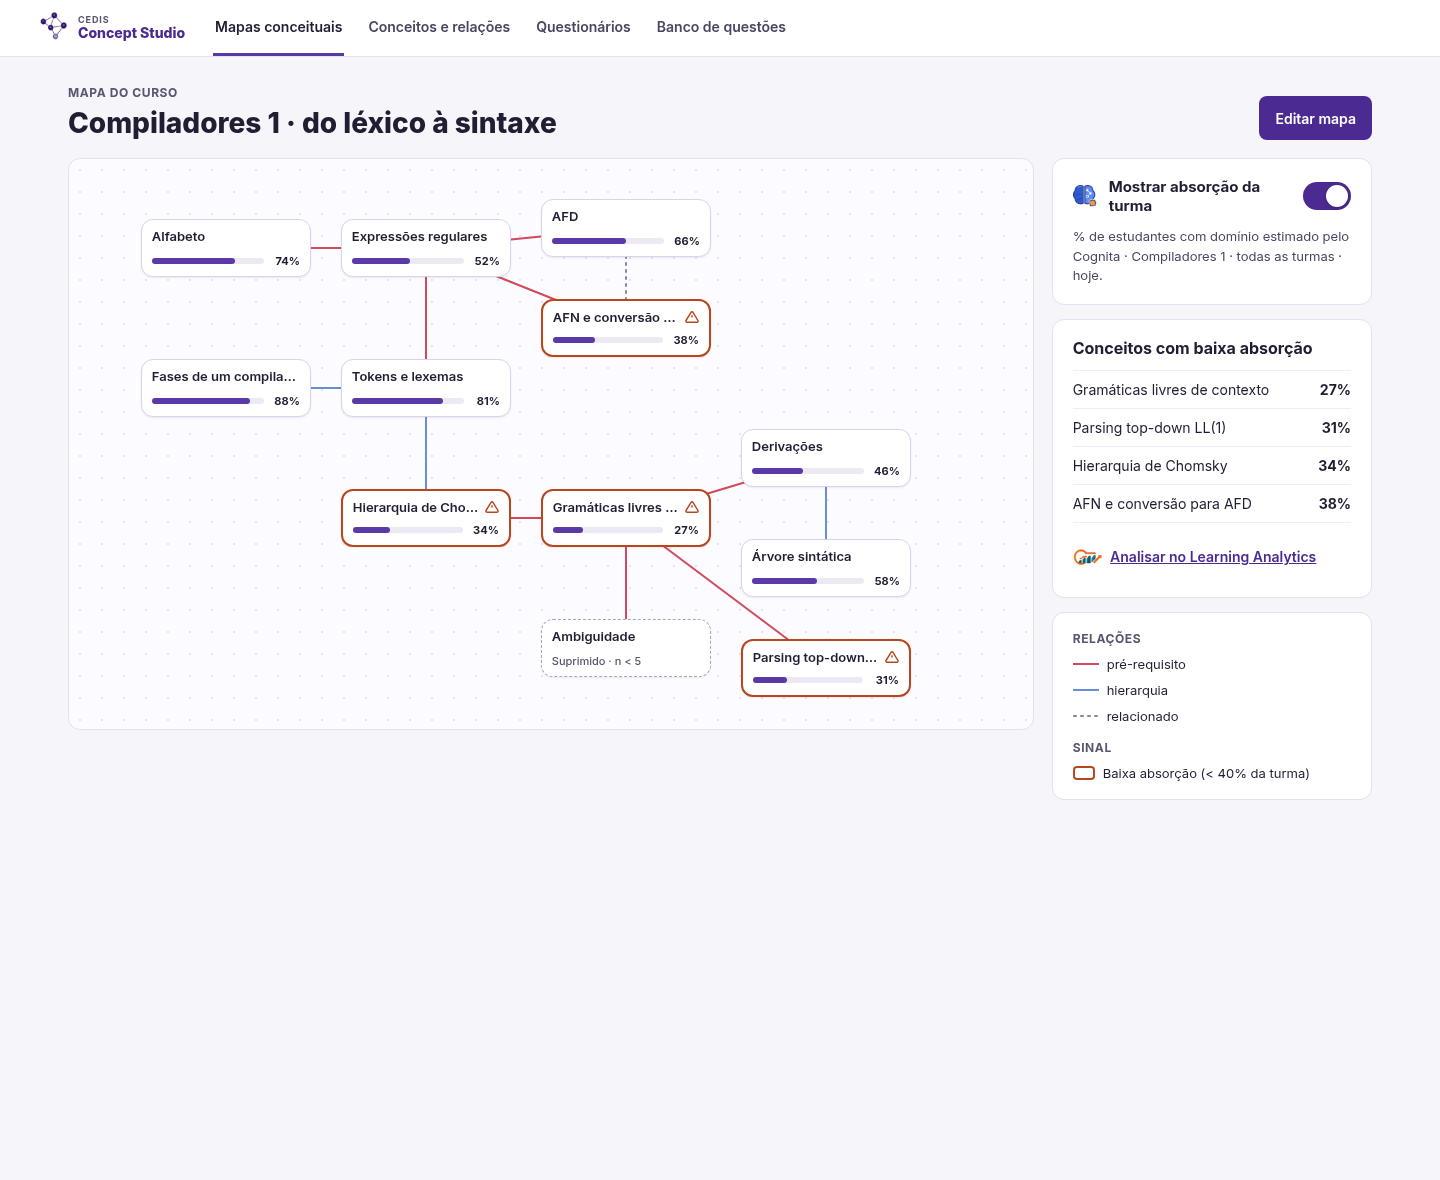
\includegraphics[width=\textwidth,height=0.72\textheight,keepaspectratio]{figuras/prototipo/concept-studio-mapa-absorcao-rf12.png}
\legend{Fonte: Elaborado pelos autores.}
\end{figure}

No Deck Manager, o Cognita ocupa duas abas. A aba \textit{Reforço por conceito}, apresentada na Figura~\ref{fig:prototipo-deck-reforco}, lista os conceitos com menor absorção e, para o conceito selecionado, indica visualmente os \textit{decks} e atividades que precisam de reforço, a partir da taxa de erro das atividades ligadas ao conceito (RF20).

\begin{figure}[H]
\caption{Protótipo dos materiais que precisam de reforço no Deck Manager (RF20)}
\label{fig:prototipo-deck-reforco}
\centering
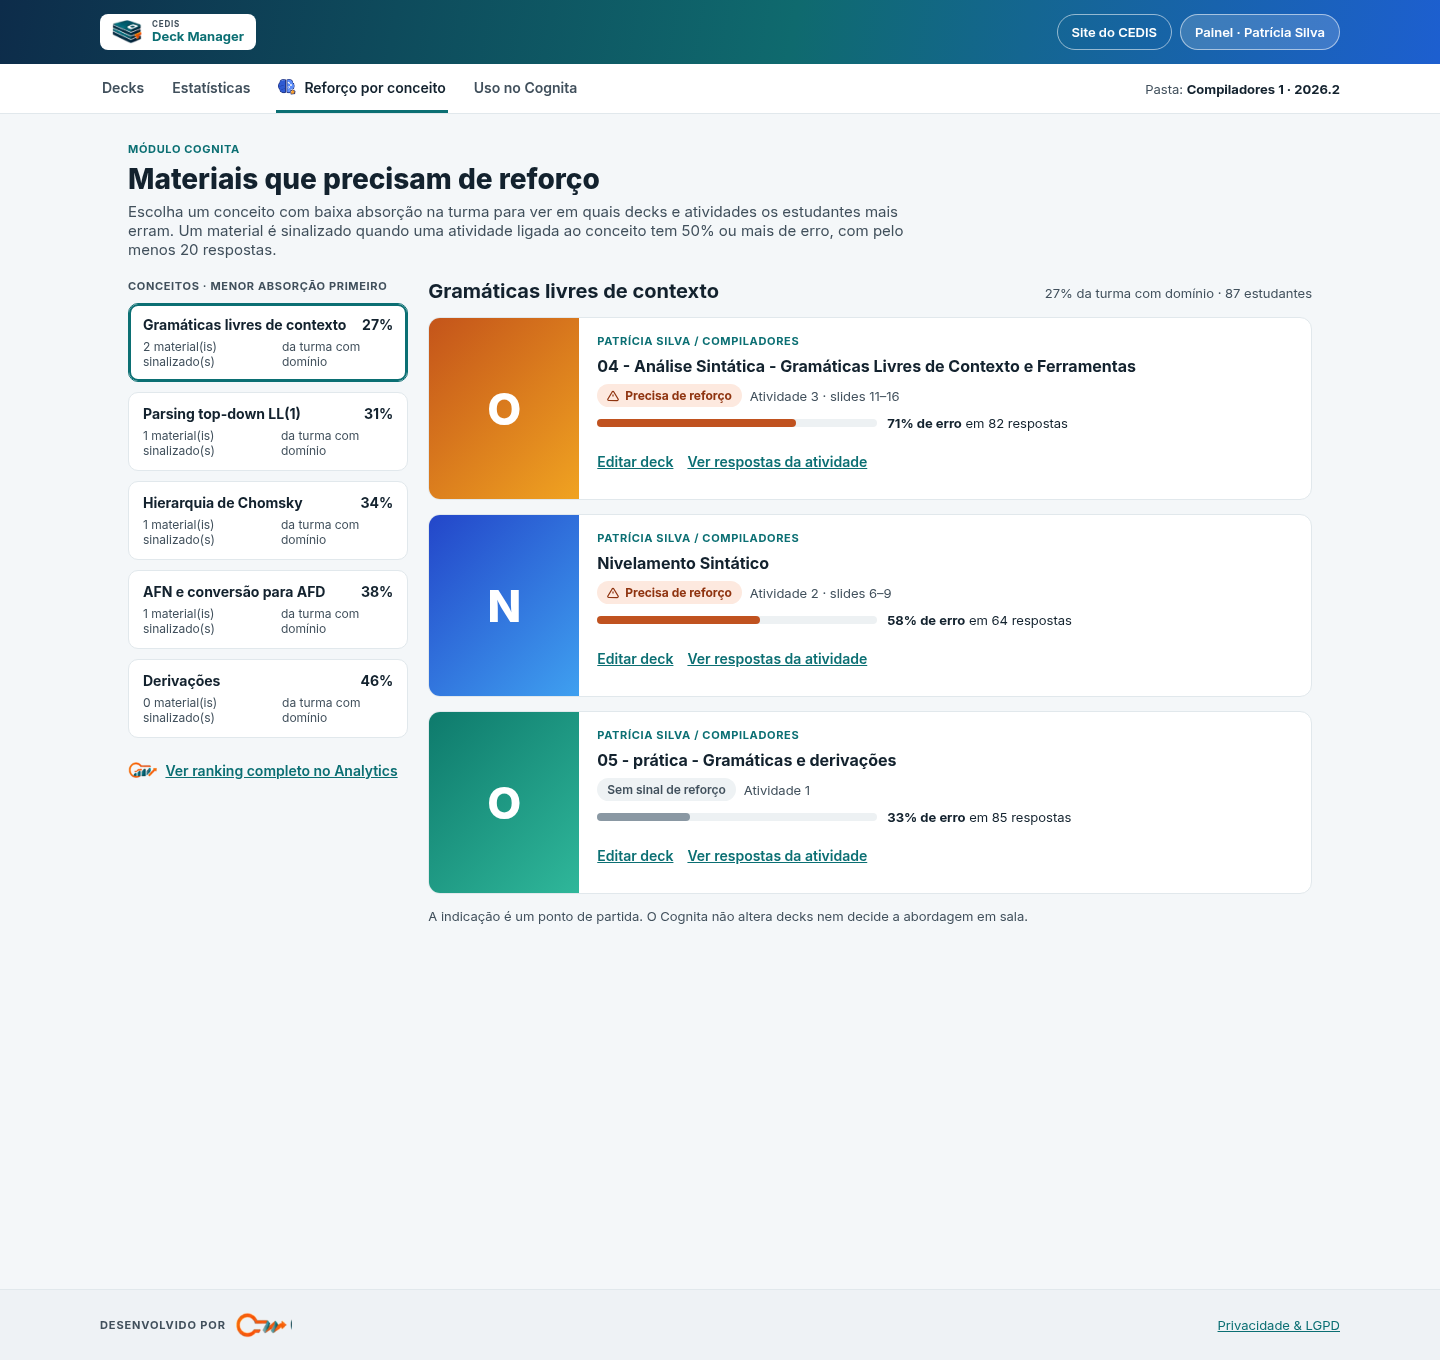
\includegraphics[width=\textwidth,height=0.72\textheight,keepaspectratio]{figuras/prototipo/deck-manager-materiais-reforco-rf20.png}
\legend{Fonte: Elaborado pelos autores.}
\end{figure}

Já a aba \textit{Uso no Cognita}, apresentada na Figura~\ref{fig:prototipo-deck-treino}, permite que o professor defina quais \textit{decks} da sua pasta serão considerados no treinamento do modelo (RF04). \textit{Decks} sem atividades vinculadas a conceitos ficam indisponíveis, e \textit{decks} com mapeamento parcial podem ser retirados do treino até que o mapeamento seja concluído, evitando que materiais em construção afetem as estimativas.

\begin{figure}[H]
\caption{Protótipo da seleção dos \textit{decks} considerados no treinamento no Deck Manager (RF04)}
\label{fig:prototipo-deck-treino}
\centering
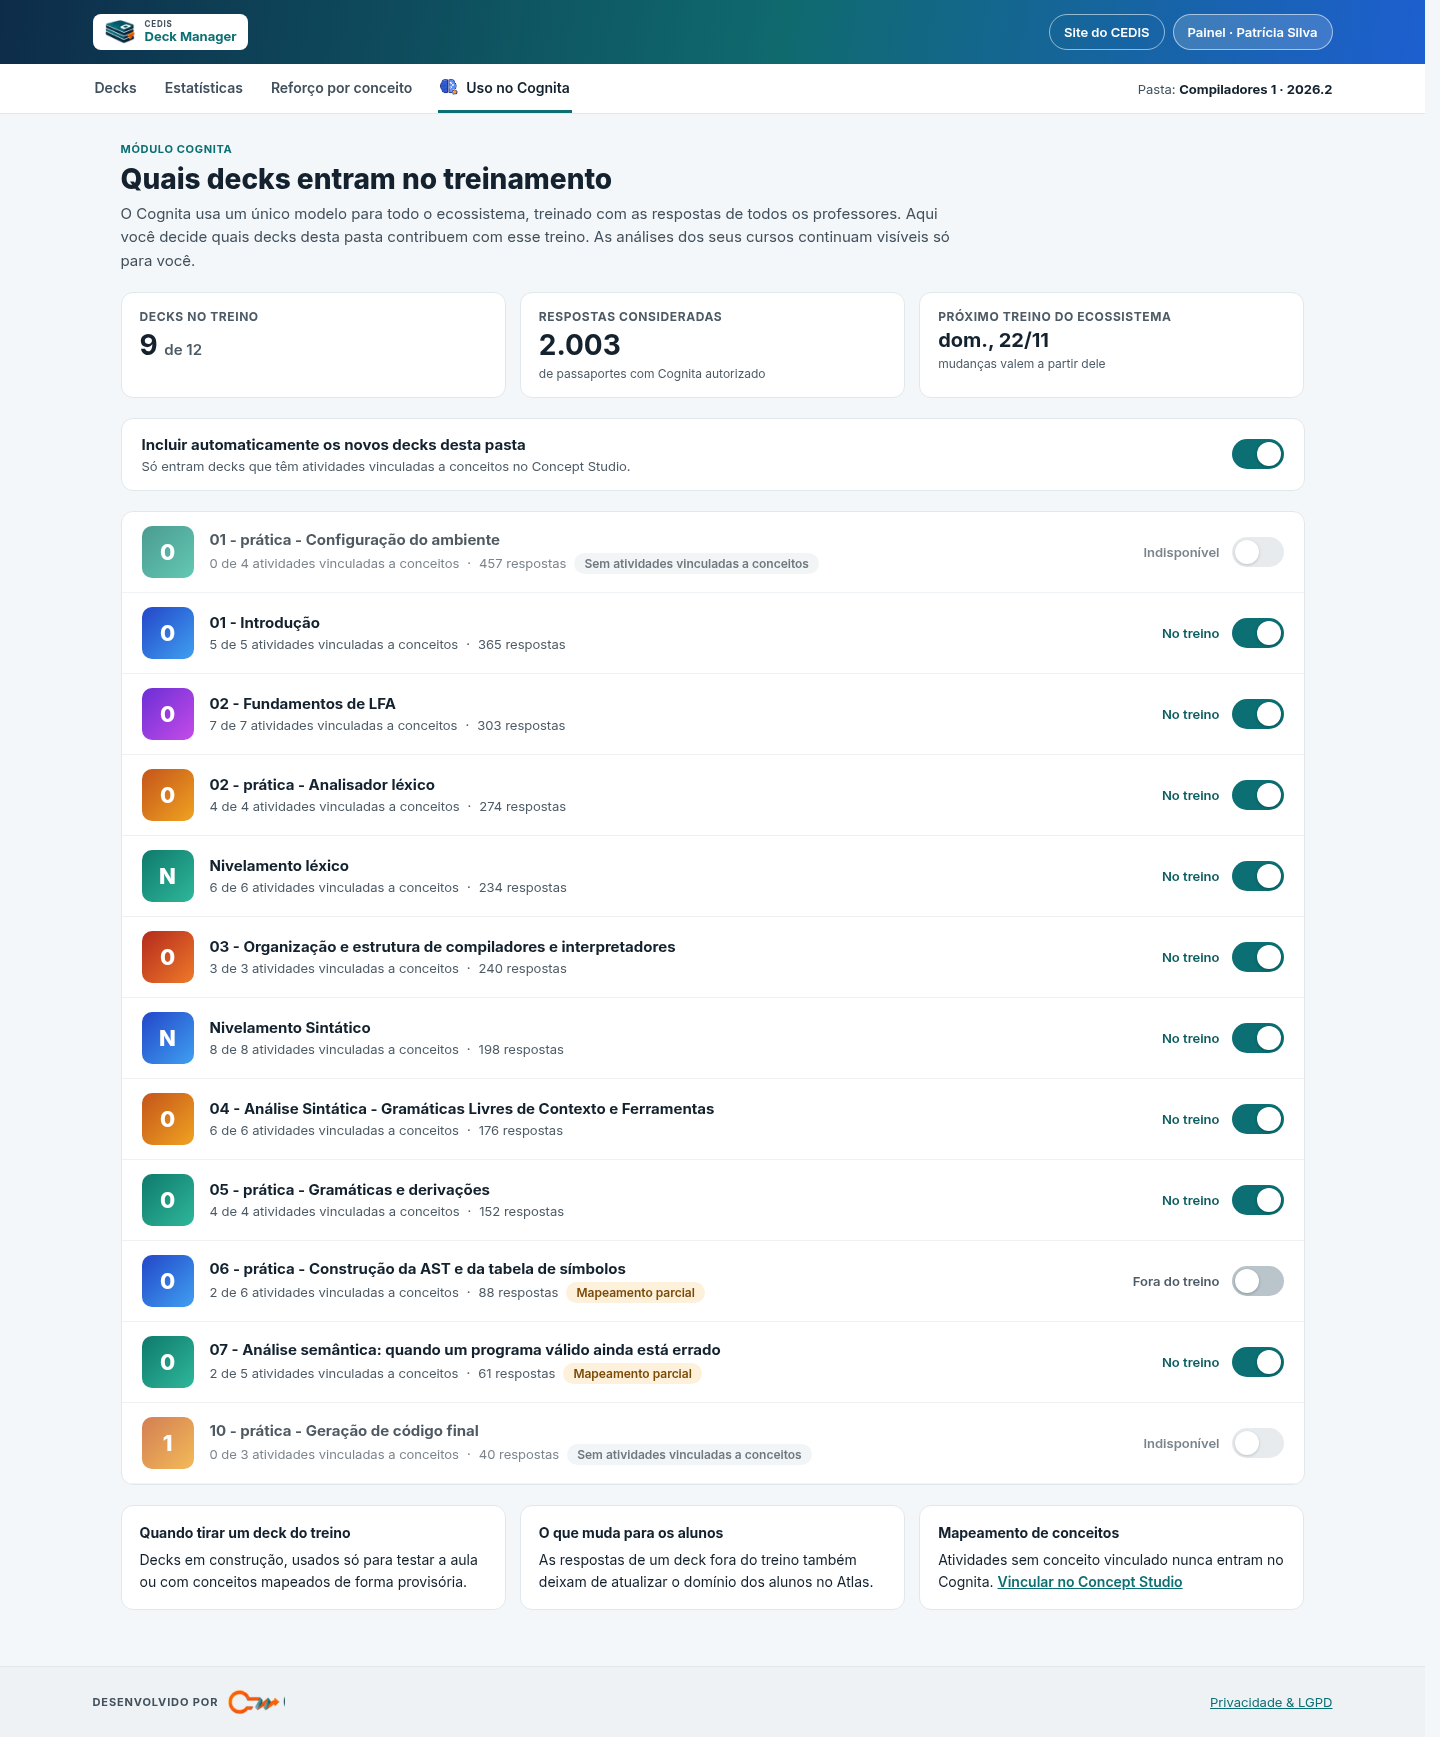
\includegraphics[width=\textwidth,height=0.72\textheight,keepaspectratio]{figuras/prototipo/deck-manager-uso-decks-rf04.png}
\legend{Fonte: Elaborado pelos autores.}
\end{figure}

\subsection{Privacidade dos Dados}
\label{subsec:prototipo-privacidade}

Por fim, a Figura~\ref{fig:prototipo-passport} apresenta a página \textit{Meus dados} do Learning Passport, onde o usuário controla o uso dos seus dados pelo Cognita. A chave \textit{Usar minhas respostas para estimar meu domínio} representa o consentimento ativo exigido pelo RNF14, e a opção \textit{Solicitar exclusão} permite apagar as estimativas de domínio e o histórico associados ao passaporte (RF24), dentro do prazo definido pelo RNF16, sem afetar os demais dados do estudante no ecossistema.

\begin{figure}[H]
\caption{Protótipo da página \textit{Meus dados} no Learning Passport (RF24, RNF14 e RNF16)}
\label{fig:prototipo-passport}
\centering
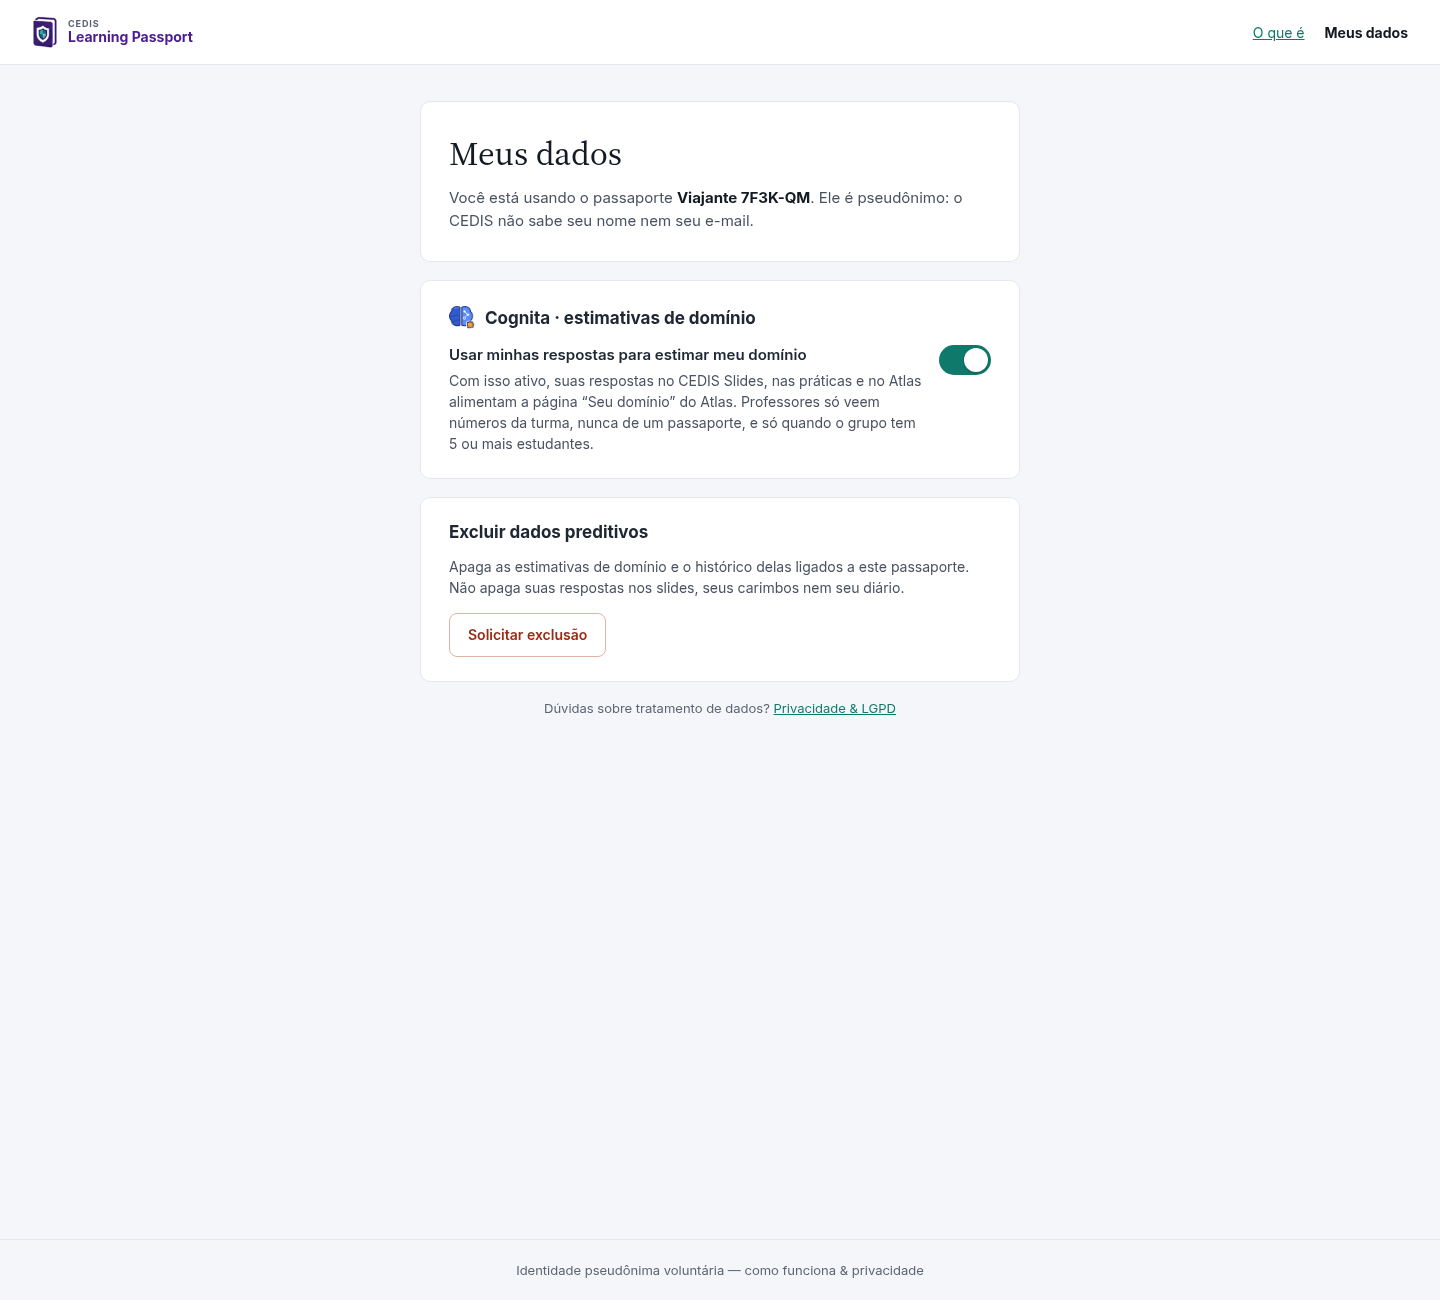
\includegraphics[width=0.85\textwidth,height=0.72\textheight,keepaspectratio]{figuras/prototipo/passport-meus-dados-rf24-rnf14-rnf16.png}
\legend{Fonte: Elaborado pelos autores.}
\end{figure}


\section{Cronograma de Desenvolvimento}
\label{sec:cronograma}

O desenvolvimento do Cognita será conduzido em onze \textit{Sprints}. As
oito primeiras correspondem às ondas do MVP definidas no sequenciador da
\textit{Lean Inception}; os incrementos
não serão entregues no desenvolvimento. A nona \textit{Sprint} é
reservada para testes e correções, e as duas últimas, para o congelamento de código
(\textit{code freeze}). A Tabela~\ref{tab:cronograma-ondas} associa cada
\textit{Sprint} aos requisitos entregues, ao escopo da entrega e ao período
de execução.

{\small
\begin{longtable}{c>{\raggedright\arraybackslash}p{2.3cm}>{\raggedright\arraybackslash}p{6.3cm}cc}
\caption{Cronograma de desenvolvimento por \textit{Sprints}}
\label{tab:cronograma-ondas} \\
\hline
\textbf{\textit{Sprint}} & \textbf{Requisitos (código)} & \textbf{Escopo da entrega} & \textbf{Início} & \textbf{Término} \\
\hline
\endfirsthead
\caption[]{Cronograma de desenvolvimento por \textit{Sprints} (continuação)} \\
\hline
\textbf{\textit{Sprint}} & \textbf{Requisitos (código)} & \textbf{Escopo da entrega} & \textbf{Início} & \textbf{Término} \\
\hline
\endhead
\hline
\multicolumn{5}{r}{\textit{Continua na próxima página}} \\
\endfoot
\hline
\multicolumn{5}{l}{Fonte: Elaborado pelos autores.} \\
\endlastfoot
1 & RF01, RF03, RF06 & Validação dos dados, treinamento inicial do modelo e probabilidade de domínio no Atlas. & 15/02/2027 & 25/02/2027 \\
\hline
2 & RF02, RF04, RF16 & Retreinamento e política de treino do modelo; confiança das estimativas no Atlas. & 26/02/2027 & 09/03/2027 \\
\hline
3 & RF12, RF17 & Explicação das estimativas no Atlas e identificação de conceitos com baixa absorção. & 10/03/2027 & 20/03/2027 \\
\hline
4 & RF08, RF13, RF18 & Conceitos a revisar no Atlas; ranking de absorção e confiança das estimativas no Analytics. & 22/03/2027 & 01/04/2027 \\
\hline
5 & RF07, RF09 & Atualização das estimativas por interação e histórico por conceito. & 02/04/2027 & 13/04/2027 \\
\hline
6 & RF05, RF19 & Métricas de predição por treinamento e explicação das estimativas no Analytics. & 14/04/2027 & 24/04/2027 \\
\hline
7 & RF11, RF20, RF24 & Proporção de estudantes com domínio, materiais para reforço e exclusão de dados do passaporte. & 26/04/2027 & 06/05/2027 \\
\hline
8 & RF10, RF15 & Evolução da absorção ao longo do tempo e filtros de resultados no Analytics, concluindo o MVP. & 07/05/2027 & 18/05/2027 \\
\hline
9 & Nenhum & Reservada para testes e correções. & 19/05/2027 & 29/05/2027 \\
\hline
10 & Nenhum & \textit{Code freeze}. & 31/05/2027 & 10/06/2027 \\
\hline
11 & Nenhum & \textit{Code freeze}. & 11/06/2027 & 22/06/2027 \\
\hline
\end{longtable}
}
